\documentclass[a4paper,12pt,twoside]{memoir}

% Castellano
\usepackage[spanish,es-tabla]{babel}
\selectlanguage{spanish}
\usepackage[utf8]{inputenc}
\usepackage[T1]{fontenc}
\usepackage{lmodern} % scalable font
\usepackage{microtype}
\usepackage{placeins}

\RequirePackage{booktabs}
\RequirePackage[table]{xcolor}
\RequirePackage{xtab}
\RequirePackage{multirow}

% Links
\PassOptionsToPackage{hyphens}{url}\usepackage[colorlinks]{hyperref}
\hypersetup{
	allcolors = {red}
}

% Ecuaciones
\usepackage{amsmath}

% Rutas de fichero / paquete
\newcommand{\ruta}[1]{{\sffamily #1}}

% Párrafos
\nonzeroparskip

% Huérfanas y viudas
\widowpenalty100000
\clubpenalty100000

% Evitar solapes en el header
\nouppercaseheads


% Imagenes
\usepackage{graphicx}
\newcommand{\imagen}[2]{
	\begin{figure}[!h]
		\centering
		\includegraphics[width=0.9\textwidth]{#1}
		\caption{#2}\label{fig:#1}
	\end{figure}
	\FloatBarrier
}

\newcommand{\imagenflotante}[2]{
	\begin{figure}%[!h]
		\centering
		\includegraphics[width=0.9\textwidth]{#1}
		\caption{#2}\label{fig:#1}
	\end{figure}
}



% El comando \figura nos permite insertar figuras comodamente, y utilizando
% siempre el mismo formato. Los parametros son:
% 1 -> Porcentaje del ancho de página que ocupará la figura (de 0 a 1)
% 2 --> Fichero de la imagen
% 3 --> Texto a pie de imagen
% 4 --> Etiqueta (label) para referencias
% 5 --> Opciones que queramos pasarle al \includegraphics
% 6 --> Opciones de posicionamiento a pasarle a \begin{figure}
\newcommand{\figuraConPosicion}[6]{%
  \setlength{\anchoFloat}{#1\textwidth}%
  \addtolength{\anchoFloat}{-4\fboxsep}%
  \setlength{\anchoFigura}{\anchoFloat}%
  \begin{figure}[#6]
    \begin{center}%
      \Ovalbox{%
        \begin{minipage}{\anchoFloat}%
          \begin{center}%
            \includegraphics[width=\anchoFigura,#5]{#2}%
            \caption{#3}%
            \label{#4}%
          \end{center}%
        \end{minipage}
      }%
    \end{center}%
  \end{figure}%
}

%
% Comando para incluir imágenes en formato apaisado (sin marco).
\newcommand{\figuraApaisadaSinMarco}[5]{%
  \begin{figure}%
    \begin{center}%
    \includegraphics[angle=90,height=#1\textheight,#5]{#2}%
    \caption{#3}%
    \label{#4}%
    \end{center}%
  \end{figure}%
}
% Para las tablas
\newcommand{\otoprule}{\midrule [\heavyrulewidth]}
%
% Nuevo comando para tablas pequeñas (menos de una página).
\newcommand{\tablaSmall}[5]{%
 \begin{table}
  \begin{center}
   \rowcolors {2}{gray!35}{}
   \begin{tabular}{#2}
    \toprule
    #4
    \otoprule
    #5
    \bottomrule
   \end{tabular}
   \caption{#1}
   \label{tabla:#3}
  \end{center}
 \end{table}
}

%
%Para el float H de tablaSmallSinColores
\usepackage{float}

%
% Nuevo comando para tablas pequeñas (menos de una página).
\newcommand{\tablaSmallSinColores}[5]{%
 \begin{table}[H]
  \begin{center}
   \begin{tabular}{#2}
    \toprule
    #4
    \otoprule
    #5
    \bottomrule
   \end{tabular}
   \caption{#1}
   \label{tabla:#3}
  \end{center}
 \end{table}
}

\newcommand{\tablaApaisadaSmall}[5]{%
\begin{landscape}
  \begin{table}
   \begin{center}
    \rowcolors {2}{gray!35}{}
    \begin{tabular}{#2}
     \toprule
     #4
     \otoprule
     #5
     \bottomrule
    \end{tabular}
    \caption{#1}
    \label{tabla:#3}
   \end{center}
  \end{table}
\end{landscape}
}

%
% Nuevo comando para tablas grandes con cabecera y filas alternas coloreadas en gris.
\newcommand{\tabla}[6]{%
  \begin{center}
    \tablefirsthead{
      \toprule
      #5
      \otoprule
    }
    \tablehead{
      \multicolumn{#3}{l}{\small\sl continúa desde la página anterior}\\
      \toprule
      #5
      \otoprule
    }
    \tabletail{
      \hline
      \multicolumn{#3}{r}{\small\sl continúa en la página siguiente}\\
    }
    \tablelasttail{
      \hline
    }
    \bottomcaption{#1}
    \rowcolors {2}{gray!35}{}
    \begin{xtabular}{#2}
      #6
      \bottomrule
    \end{xtabular}
    \label{tabla:#4}
  \end{center}
}

%
% Nuevo comando para tablas grandes con cabecera.
\newcommand{\tablaSinColores}[6]{%
  \begin{center}
    \tablefirsthead{
      \toprule
      #5
      \otoprule
    }
    \tablehead{
      \multicolumn{#3}{l}{\small\sl continúa desde la página anterior}\\
      \toprule
      #5
      \otoprule
    }
    \tabletail{
      \hline
      \multicolumn{#3}{r}{\small\sl continúa en la página siguiente}\\
    }
    \tablelasttail{
      \hline
    }
    \bottomcaption{#1}
    \begin{xtabular}{#2}
      #6
      \bottomrule
    \end{xtabular}
    \label{tabla:#4}
  \end{center}
}

%
% Nuevo comando para tablas grandes sin cabecera.
\newcommand{\tablaSinCabecera}[5]{%
  \begin{center}
    \tablefirsthead{
      \toprule
    }
    \tablehead{
      \multicolumn{#3}{l}{\small\sl continúa desde la página anterior}\\
      \hline
    }
    \tabletail{
      \hline
      \multicolumn{#3}{r}{\small\sl continúa en la página siguiente}\\
    }
    \tablelasttail{
      \hline
    }
    \bottomcaption{#1}
  \begin{xtabular}{#2}
    #5
   \bottomrule
  \end{xtabular}
  \label{tabla:#4}
  \end{center}
}



\definecolor{cgoLight}{HTML}{EEEEEE}
\definecolor{cgoExtralight}{HTML}{FFFFFF}

%
% Nuevo comando para tablas grandes sin cabecera.
\newcommand{\tablaSinCabeceraConBandas}[5]{%
  \begin{center}
    \tablefirsthead{
      \toprule
    }
    \tablehead{
      \multicolumn{#3}{l}{\small\sl continúa desde la página anterior}\\
      \hline
    }
    \tabletail{
      \hline
      \multicolumn{#3}{r}{\small\sl continúa en la página siguiente}\\
    }
    \tablelasttail{
      \hline
    }
    \bottomcaption{#1}
    \rowcolors[]{1}{cgoExtralight}{cgoLight}

  \begin{xtabular}{#2}
    #5
   \bottomrule
  \end{xtabular}
  \label{tabla:#4}
  \end{center}
}




\graphicspath{ {./img/} }

% Capítulos
\chapterstyle{bianchi}
\newcommand{\capitulo}[2]{
	\setcounter{chapter}{#1}
	\setcounter{section}{0}
	\setcounter{figure}{0}
	\setcounter{table}{0}
	\chapter*{#2}
	\addcontentsline{toc}{chapter}{#2}
	\markboth{#2}{#2}
}

% Apéndices
\renewcommand{\appendixname}{Apéndice}
\renewcommand*\cftappendixname{\appendixname}

\newcommand{\apendice}[1]{
	%\renewcommand{\thechapter}{A}
	\chapter{#1}
}

\renewcommand*\cftappendixname{\appendixname\ }

% Formato de portada
\makeatletter
\usepackage{xcolor}
\newcommand{\tutor}[1]{\def\@tutor{#1}}
\newcommand{\course}[1]{\def\@course{#1}}
\definecolor{cpardoBox}{HTML}{E6E6FF}
\def\maketitle{
  \null
  \thispagestyle{empty}
  % Cabecera ----------------
\noindent
\includegraphics[width=\textwidth]{cabecera}\vspace{1cm}%
  \vfill
  % Título proyecto y escudo informática ----------------
  \colorbox{cpardoBox}{%
    \begin{minipage}{.8\textwidth}
      \vspace{.5cm}\Large
      \begin{center}
      \textbf{TFG del Grado en Ingeniería Informática}\vspace{.6cm}\\
      \textbf{\LARGE\@title{}}
      \end{center}
      \vspace{.2cm}
    \end{minipage}

  }%
  \hfill\begin{minipage}{.20\textwidth}
    
\includegraphics[width=\textwidth]{escudoInfor}
  \end{minipage}
  \vfill
  % Datos de alumno, curso y tutores ------------------
  \begin{center}%
  {%
    \noindent\LARGE
    Presentado por \@author{}\\ 
    en Universidad de Burgos --- \@date{}\\
    Tutores: \@tutor{}\\
  }%
  \end{center}%
  \null
  \cleardoublepage
  }
\makeatother


% Datos de portada
\title{Aplicación de gestión del PDI de áreas de conocimiento en universidades  \\Documentación Técnica}
\author{Ignacio Dávila García}
\tutor{Álvar Arnaiz González y Carlos Pardo Aguilar}
\date{\today}

\begin{document}

\maketitle



\cleardoublepage



%%%%%%%%%%%%%%%%%%%%%%%%%%%%%%%%%%%%%%%%%%%%%%%%%%%%%%%%%%%%%%%%%%%%%%%%%%%%%%%%%%%%%%%%



\frontmatter


\clearpage

% Indices
\tableofcontents

\clearpage

\listoffigures

\clearpage

\listoftables

\clearpage

\mainmatter

\appendix

\apendice{Plan de Proyecto Software}

\section{Introducción}
En este anexo se va a exponer la planificación temporal y el estudio de viabilidad del proyecto.

La planificación temporal está dividida en los \textit{sprints} seguidos para la realización del proyecto.
Cada apartado dentro de la planificación cuenta con información sobre la reunión de planificación del \textit{sprint}, de la que se obtienen conjunto de tareas a realizar, y la reunión de revisión, donde se muestra y valora el trabajo realizado.

\section{Planificación temporal}
Durante este proyecto se ha seguido una metodología Scrum con algunos cambios ya que no se hacían reuniones diarias ni los roles estaban tan marcados, pero la forma de trabajar era la misma con planificaciones y revisiones de \textit{sprints}.
Los \textit{sprints} que se han realizado son los siguientes:

\subsubsection{\textit{Sprint} 1: \textit{Sprint} inicial}
Fechas: 28 febrero 2023 -- 7 marzo 2023.
\begin{itemize}
\item\textbf{Planificación del \textit{sprint}}

En la reunión de planificación del sprint se fijaron las siguientes tareas:
\begin{enumerate}
	\item Configuración inicial del repositorio
	\item Prototipos de las vistas de la aplicación
	\item Creación diagrama entidad-relación
\end{enumerate}

\item\textbf{\textit{Burndown Report}}

\begin{figure}
	\centering
	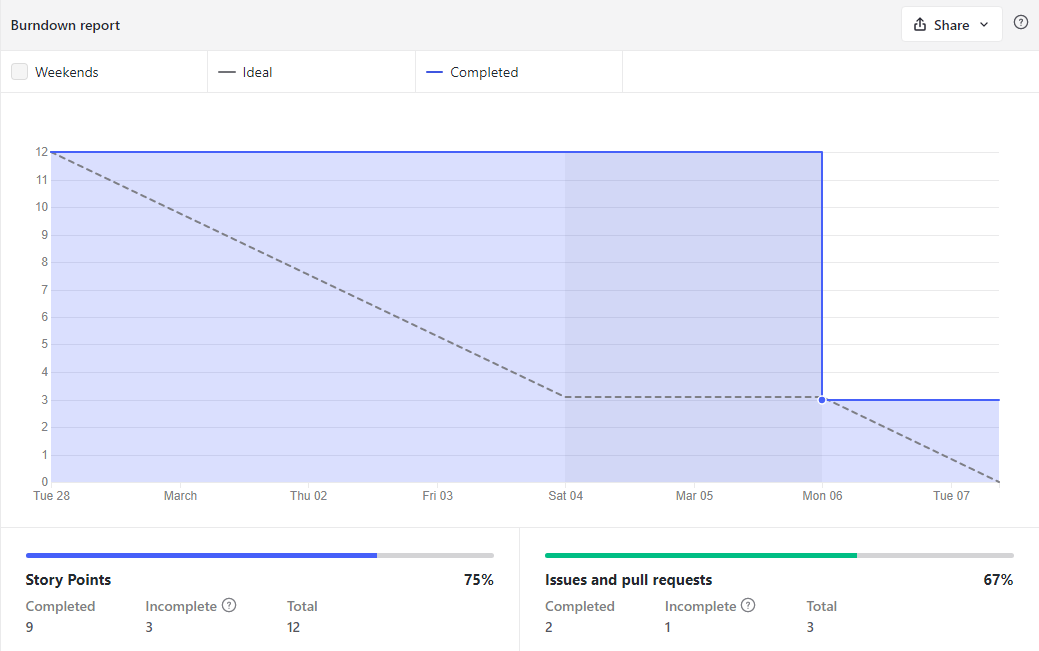
\includegraphics[width=\textwidth]{../img/Anexos/Sprints/Sprint1.png}
	\caption{\textit{Burndown Report Sprint 1}}\label{ReportSprint1}
\end{figure}

Como se puede apreciar en la figura~\ref{ReportSprint1}, no todas las tareas aparecen como completadas. Esto es debido a que el diagrama entidad-relación se dejó abierto ya que faltaba información para completarlo.

\item\textbf{Revisión del \textit{sprint}}

Durante la revisión se mostró el trabajo realizado y se vieron los cambios que se debían realizar en el diagrama entidad-relación que a su vez implicaban cambios en los prototipos de las vistas de la aplicación.
Se llegó a la conclusión de que podía ser buena idea dividir el diagrama E/R haciendo vistas del mismo para que fuere más fácil resolverlo.
\end{itemize}


\subsubsection{\textit{Sprint} 2: Casos de uso y diagrama E/R de cada caso}
Fechas: 7 marzo 2023 -- 14 marzo 2023.
\begin{itemize}
\item\textbf{Planificación del \textit{sprint}}

En la reunión de planificación del sprint se fijaron las siguientes tareas:
\begin{enumerate}
	\item Creación de casos de uso junto a su vista del diagrama E/R.
	\item Aprendizaje de Flask.
\end{enumerate}

\item\textbf{\textit{Burndown Report}}

\begin{figure}
	\centering
	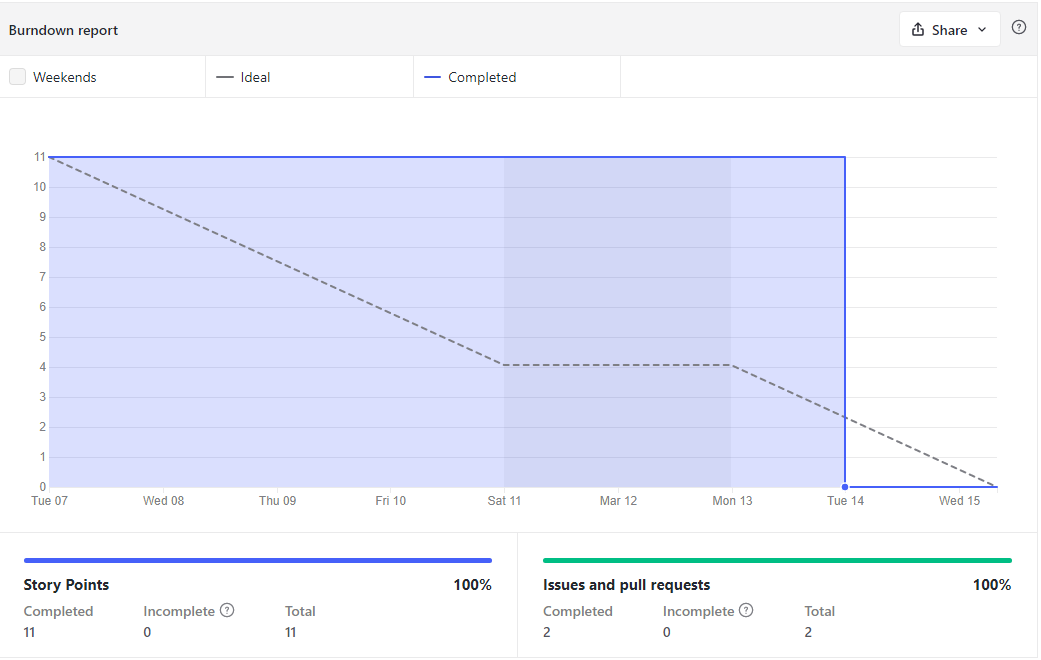
\includegraphics[width=\textwidth]{../img/Anexos/Sprints/Sprint2.png}
	\caption{\textit{Burndown Report Sprint 2}}\label{ReportSprint2}
\end{figure}

En este \textit{sprint} se completaron las tareas marcadas en el tiempo fijado durante la reunión de planificación, pero muchas cosas quedaron pendientes de cambios en futuros \textit{sprints}. En la figura~\ref{ReportSprint2} se puede ver el \textit{Burndown Report} del \textit{sprint}.

\item\textbf{Revisión del \textit{sprint}}

En la reunión de revisión se estudió de nuevo el diagrama E/R y se indicaron nuevos cambios menores en el mismo. También se propuso el comenzar a realizar el diagrama de casos de uso y continuar con el estudio de Flask.
\end{itemize}

\subsubsection{\textit{Sprint} 3: Documentación de casos de uso e investigación y aprendizaje de Flask y bibliotecas JavaScript}
Fechas: 14 marzo 2023 -- 21 marzo 2023.
\begin{itemize}
\item\textbf{Planificación del \textit{sprint}}

En la reunión de planificación del sprint se fijaron las siguientes tareas:
\begin{enumerate}
		\item Realizar el diagrama de casos de uso
		\item Cambios en las vistas adaptándolas a los casos de uso
		\item Documentar los casos de uso con sus tablas
		\item Investigar bibliotecas de JavaScript que pudiesen ayudar
		\item Aprender sobre Flask
\end{enumerate}

\item\textbf{\textit{Burndown Report}}

\begin{figure}
	\centering
	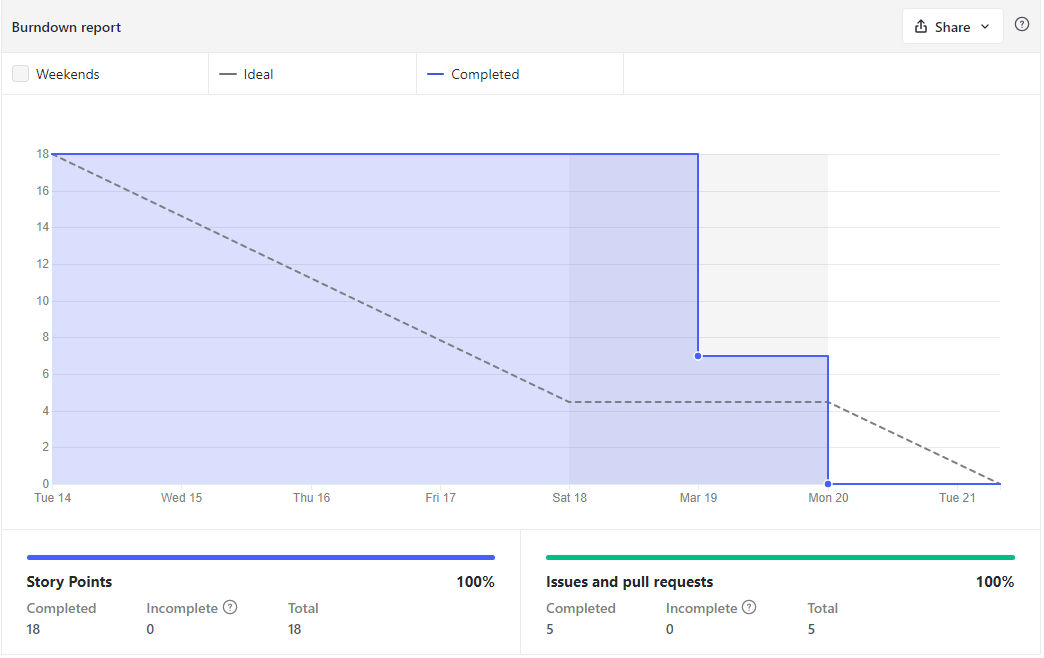
\includegraphics[width=\textwidth]{../img/Anexos/Sprints/Sprint3.png}
	\caption{\textit{Burndown Report Sprint 3}}\label{ReportSprint3}
\end{figure}

En este \textit{sprint} se completaron las tareas marcadas aunque el tiempo marcado para el aprendizaje de Flask fue menor debido a falta de tiempo durante esta semana. Estaba previsto dedicar en total 18 horas al \textit{sprint}, pero finalmente fueron 15. En la figura~\ref{ReportSprint3} se puede ver el \textit{Burndown Report} del \textit{sprint}.

\item\textbf{Revisión del \textit{sprint}}

Durante la revisión se vio que había casos de uso que no eran necesarios y que se podían añadir como excepciones de otros. Esto produjo que el diagrama de casos de uso se debía cambiar, lo que implica un cambio en la documentación de las tablas y en los prototipos de las vistas de la aplicación.
\end{itemize}

\subsubsection{\textit{Sprint} 4: Cambios en los casos de uso y vistas, documentación y Flask}
Fechas: 21 marzo 2023 -- 28 marzo 2023.
\begin{itemize}
\item\textbf{Planificación del \textit{sprint}}

En la reunión de planificación del sprint se fijaron las siguientes tareas:
\begin{enumerate}
		\item Cambios en el diagrama de casos de uso dividiendo en diagrama por niveles y crear vistas del diagrama E/R para los casos de uso.
		\item Cambios en algunos prototipos de las vistas de la aplicación.
		\item Cambios en la documentación de los casos de uso (tablas).
		\item Añadir documentación.
		\item Comenzar estructura básica de la aplicación en Flask.
\end{enumerate}

\item\textbf{\textit{Burndown Report}}

\begin{figure}
	\centering
	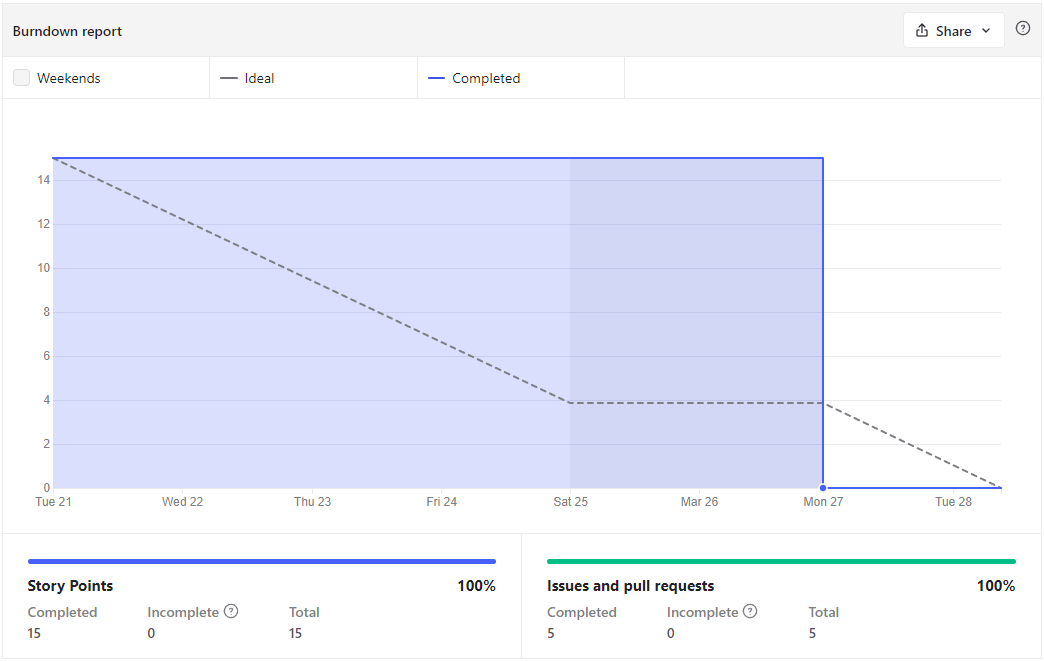
\includegraphics[width=\textwidth]{../img/Anexos/Sprints/Sprint4.png}
	\caption{\textit{Burndown Report Sprint 4}}\label{ReportSprint4}
\end{figure}

A lo largo del \textit{sprint} se realizaron la mayoría de tareas marcadas, pero en las tareas de añadir documentación y comenzar con Flask, no se hizo tanto como estaba esperado debido a la falta de tiempo. 
Se planeo que se iban a poder dedicar más horas de las que al final se dedicaron y no se avanzó todo lo planeado en estas tareas. 
Aún así, se decidió cerrarlas, ya que algo si se había avanzado, y crear de nuevo tareas similares en próximos \textit{sprints}.

La tarea de <<Cambios en el diagrama de casos de uso dividiendo en diagrama por niveles y crear vistas del diagrama E/R para los casos de uso>> tenía una previsión de 2 horas que se realizó en el plazo estimado, la tarea <<Cambios en algunos prototipos de las vistas de la aplicación>> tenía una estimación de 3 horas aunque finalmente fueron 4, la tarea <<Cambios en la documentación de los casos de uso (tablas)>> tenía marcada 4 horas de duración que finalmente fueron 5, la tarea de <<Añadir documentación>> tenía pensada una dedicación de 3 horas que al final se quedó en 1 hora y media aproximadamente y, por último, la tarea <<Comenzar estructura básica de la aplicación en Flask.>> tenía una previsión de 3 horas que quedó reducida a una media hora por falta de tiempo durante el \textit{sprint}. 
En la figura~\ref{ReportSprint4} se puede ver el \textit{Burndown Report} del \textit{sprint}.

\item\textbf{Revisión del \textit{sprint}}

En la reunión de revisión del \textit{sprint} se decidió hacer algunos cambios en los casos de uso, lo que implica un cambio en la documentación de las tablas y los prototipos de las vistas ya que el funcionamiento esperado de la aplicación cambia. También se decidió realizar algún cambio en el diagrama E/R añadiendo nuevos atributos y sacando un atributo a una nueva entidad.
\end{itemize}

\subsubsection{\textit{Sprint} 5: Documentación y comienzo de la aplicación}
Fechas: 28 marzo 2023 -- 11 abril 2023.
\begin{itemize}
\item\textbf{Planificación del \textit{sprint}}

En la reunión de planificación del sprint se fijaron las siguientes tareas:
\begin{enumerate}
		\item Cambios en el diagrama E/R y en algún caso de uso.
		\item Cambios en algunas tablas de los CU y en sus respectivas vistas.
		\item Evaluar plugins/frameworsk para tablas.
		\item Añadir documentación.
		\item Desarrollo de la aplicación.
\end{enumerate}

\item\textbf{\textit{Burndown Report}}

En este \textit{sprint} surgió un problema con herramienta ZenHub que utilizaba para llevar un seguimiento de los \textit{sprints} desde GitHub. Es una herramienta de pago que en teoría cuenta con versiones gratuitas para proyectos \textit{open source} y para profesores. Contacté con ellos para poder obtener una licencia gratuita de la herramienta, pero no fue posible conseguirla. Por lo tanto, a partir de este \textit{sprint} no pude utilizar la herramienta y no pude sacar la imagen del \textit{Burndown Report}.

Para la tarea de <<Cambios en el diagrama E/R y en algún caso de uso>> se estimaba un tiempo de realización de 1 hora que se cumplió.

Para la tarea <<Cambios en algunas tablas de los CU y en sus respectivas vistas>> se puso una estimación de 5 horas que finalmente fueron 7 horas.

Para la tarea <<Evaluar plugins/frameworsk para tablas>> se había marcado una planificación de 2 horas que se cumplió, excediendo un poco de la planificación, ya que aparte de buscar y valorar distintas librerías de JavaScript para la visualización de tablas estuve haciendo pruebas con la librería Grid.js que decidí utilizar para el proyecto.

La tarea de <<Añadir documentación>> tenía marcada una planificación de 3 horas que se cumplió dentro del plazo.

Por último, la tarea de <<Desarrollo de la aplicación>>, donde se buscaba empezar con la aplicación web, tenía una estimación de 8 horas que se convirtió en unas 10 horas de trabajo real debido a algunos problemas surgidos durante el desarrollo.

\item\textbf{Revisión del \textit{sprint}}

En la reunión de revisión se estuvo viendo el trabajo realizado durante el \textit{sprint}. En la parte de documentación se decidió que se debían hacer algunos pequeños cambios en las tablas de los casos de uso, la visualización de imágenes, cambios de orden en un diagrama y cambios en algún título.

En la parte de desarrollo de la aplicación web se decidió realizar algunos cambios en la visualización de tablas para que no ocupasen tanta pantalla así como en el menú de la web para hacerlo más pequeño introduciendo submenús. También se dijo que era mejor poner un selector de centro en la pantalla de la asignación de horas para que de esta forma ya saliesen los datos de la tabla filtrados por centro. 
\end{itemize}

\subsubsection{\textit{Sprint} 6: Base de datos y comenzar a dar funcionalidad a la web}
Fechas: 11 abril 2023 -- 24 abril 2023.
\begin{itemize}
\item\textbf{Planificación del \textit{sprint}}

En la reunión de planificación del sprint se fijaron las siguientes tareas:
\begin{enumerate}
		\item Creación de los modelos y la base de datos en base a los modelos.
		\item Crear la primera carga de la base de datos con CSV y script SQL.
		\item Creación de más vistas junto a su funcionalidad.
		\item Cambios en la documentación.
		\item Añadir más documentación.
\end{enumerate}

\item\textbf{\textit{Burndown Report}}

Este \textit{sprint} tenía una duración inicial de una semana, pero debido a falta de tiempo por exámenes y entregas de trabajos, decidí aplazar una semana más la reunión de revisión para poder trabajar en el proyecto. 
Además, se tuvo que cambiar la fecha habitual de las reuniones debido a que empecé prácticas en una empresa y ya no era compatible la hora/día que se tenía.

La primera tarea completada fue la de <<Creación de los modelos y la base de datos en base a los modelos>>. 
Se puso una estimación de 4 horas, que de trabajo real fue el doble, unas 8 horas. 
Este exceso de tiempo fue debido en gran medida a errores surgidos a la hora de crear la base de datos utilizando el \textit{ORM} SQLAlchemy. 
Los problemas eran principalmente por como hacía la carga de la base de datos que hacía que en algunos contextos estuviese disponible y en otros no, provocando errores al ejecutar la aplicación y generar las tablas de la base de datos.

La tarea <<Crear la primera carga de la base de datos con CSV y script SQL>> tenía una planificación de 2 horas y se completó en el tiempo. 
Sólo quedo pendiente el hecho de que desde la interfaz phpMyAdmin que estoy utilizando para manejar la base de datos, no fui capaz de cargar los archivos csv desde el script de SQL y tuve que cargarlos por separado desde la interfaz.

Para la tarea <<Creación de más vistas junto a su funcionalidad>> se tenía una estimación de 6 horas. 
En este caso fui bastante optimista y el trabajo real termino siendo de 9 horas.
Esto se debido en gran parte a la aparición de problemas que hicieron que tuviera que trabajar más horas de las planeadas en esta tarea.

La tarea <<Cambios en la documentación>> tenía planificadas 2 horas de trabajo. 
En horas reales termino siendo 2 horas y media aproximadamente.

Finalmente, la tarea de <<Añadir más documentación>> tenía una estimación de 1 hora y el trabajo realizado fue también de 1 hora. 
Se añadió sobre todo documentación sobre técnicas y herramientas, apartado de diseño y apartado de plan de proyecto.

\item\textbf{Revisión del \textit{sprint}}

En la reunión de revisión del \textit{sprint} 6 se estuvieron valorando los cambios realizados y las nuevas funcionalidades añadidas.
También se resolvieron algunas dudas sobre la documentación y algunas partes de la funcionalidad de la aplicación web.
Se discutieron algunos aspectos como el añadir algún nuevo campo en la base de datos para códigos internos o cómo tratar la eliminación de los centros, que hasta ahora se trataba como una eliminación en cascada, y se decidió cambiar al existir demasiado riesgo de pérdida de información por un borrado accidental o poco planificado.

\end{itemize}


\subsubsection{\textit{Sprint} 7: Creación de CRUDs y documentar}
Fechas: 24 abril 2023 -- 2 mayo 2023.
\begin{itemize}
\item\textbf{Planificación del \textit{sprint}}


En la reunión de planificación del sprint se fijaron las siguientes tareas:
\begin{enumerate}
		\item Comentarios sobre memoria y anexos.
		\item Crear el CRUD de Docentes, Plazas, Contratos, Áreas y Departamentos.
		\item Solucionar bug con las abreviaturas al modificar una asignatura.
		\item Algunos cambios en campos de la base de datos.
		\item Buscar cómo cargar un CSV desde un script de SQL en phpMyAdmin.
		\item Añadir documentación.
\end{enumerate}

\item\textbf{\textit{Burndown Report}}

La tarea de <<Comentarios sobre memoria y anexos>> fue una tarea creada por Álvar Arnaiz González para dejar las correcciones hechas en la memoria y los anexos. 
Esta tarea fue reutilizada para indicar que se iban a subir esos cambios en la documentación. 
Tenía una planificación de 30 minutos y se realizó dentro del tiempo estimado.

La tarea <<Crear el CRUD de Docentes, Plazas, Contratos, Áreas y Departamentos>> era la que tenía más carga de trabajo en este \textit{sprint} con una estimación de 8 horas que se convirtió en 11 horas de trabajo real.
Este incremento de horas se debió principalmente a problemas para configurar correctamente la biblioteca Select2 utilizando Ajax y para mantener las opciones marcadas en el campo en las modificaciones.

La tarea <<Solucionar bug con las abreviaturas al modificar una asignatura>> era debida a errores en el campo Select2 al hacer una modificación de una asignatura. 
Las abreviaturas de la asignatura aparecían bien, pero no se recuperaban de forma correcta en el servidor para saber cuales habían sido añadidas o eliminadas.
Esta tarea tenía una estimación de 1 hora y no se pretendía superar ese tiempo de trabajo, ya que en la reunión de planificación no se consideró que fuese un problema crucial debido a que en este momento no era necesario que una asignatura tuviera varias abreviaturas y podía ser cambiado por un campo de texto normal que no diese ese problema y permitiese a una asignatura tener una única abreviatura.
Al realizar la tarea anterior se tuvo un problema parecido que dio la pista para resolver este problema dejándolo totalmente subsanado.

La tarea <<Algunos cambios en campos de la base de datos>> tenía una estimación de 1 hora y se realizó dentro del plazo.
La tarea consistía en añadir nuevos campos en la base de datos, lo que suponía también hacer cambios en el código para introducir los nuevos atributos en los modelos y en los formularios.
También se cambió el borrado en cascada que tenían los centros para evitar que se eliminen centros que tengan titulaciones vinculadas.

Para la tarea <<Añadir documentación>> se estimaron 3 horas de trabajo que se cumplieron en cuanto a trabajo real.

Finalmente, para la tarea <<Buscar cómo cargar un CSV desde un script de SQL en phpMyAdmin>> se estimó 1 hora de trabajo que finalmente fue un trabajo real de 2 horas debido a que tuve que investigar por los problemas que me daba con la carga de los ficheros csv. El problema finalmente fue donde estaban colocados los csv.


\item\textbf{Revisión del \textit{sprint}}

En la reunión de revisión se mostró el trabajo realizado y se resolvieron algunas dudas acerca de la memoria y algunas partes del funcionamiento de la aplicación web.
\end{itemize}


\subsubsection{\textit{Sprint} 8: Gestión de cursos}
Fechas: 2 mayo 2023 -- 15 mayo 2023.
\begin{itemize}
\item\textbf{Planificación del \textit{sprint}}


En la reunión de planificación del sprint se fijaron las siguientes tareas:
\begin{enumerate}
		\item Subir la web a Heroku.
		\item Programar el apartado ge gestión de cursos.
		\item Hacer pequeños cambios en la web.
		\item Añadir documentación de trabajos relacionados.
\end{enumerate}

\item\textbf{\textit{Burndown Report}}

La primera tarea que se realizó fue <<Subir la web a Heroku>>.
La tarea tenía una carga de trabajo estimada en 2 horas.
Para esta tarea la estimación no fue nada correcta, ya que el trabajo real fue aproximadamente de 8 horas.
Esto fue debido principalmente a problemas a la hora de configurar el proyecto para ser reconocido por la plataforma Heroku y para configurar correctamente la base de datos. 
Surgieron un gran listado de problemas que fueron resueltos uno por uno hasta que la instalación fue satisfactoria.

Para la tarea <<Programar el apartado ge gestión de cursos>> se habían marcado 8 horas de trabajo que finalmente se convirtieron en mucho más, 20 horas de trabajo.
Esta gran discrepancia entre la planificación y el trabajo real fue debida en gran medida a la investigación y planteamiento de cómo mostrar el listado de asignaturas que se deben seleccionar a la hora de crear un curso.
Se intentó crear de la forma más cómoda para utilizar y con el menor impacto posible en el rendimiento.
También surgieron algunos problemas durante la programación que fueron subsanados pero que hicieron que el tiempo de trabajo se fuese desplazando aun más de la estimación realizada.

La siguiente tarea fue <<Hacer pequeños cambios en la web>>.
Esta tarea tenía una estimación de 3 horas que de trabajo real en realidad fueron unas 2 horas. 
Estos pequeños cambios eran principalmente sobre la visualización del contenido.

Finalmente, la tarea <<Añadir documentación de trabajos relacionados>> tenía una estimación de trabajo de 1 hora y el trabajo real tuvo también una duración aproximada de una hora.


\item\textbf{Revisión del \textit{sprint}}

Durante la reunión de revisión se vieron principalmente los cambios realizados en la web. Se estuvieron discutiendo diferentes formas de crear los cursos y se llegó a la conclusión de hacer pequeños cambios para que fuese más cómoda la creación de cursos.
También se estuvieron viendo las diferentes secciones de la memoria para dar ideas sobre la documentación que se podía ir introduciendo.
\end{itemize}


\subsubsection{\textit{Sprint} 9: Cambios, gestión de grupos y documentación}
Fechas: 15 mayo 2023 -- 23 mayo 2023.
\begin{itemize}
\item\textbf{Planificación del \textit{sprint}}


En la reunión de planificación del sprint se fijaron las siguientes tareas:
\begin{enumerate}
		\item Algunos cambios en la gestión de cursos.
		\item Creación de la gestión de grupos.
		\item Pequeños cambios/mejoras en el código.
		\item Avanzar en la memoria.
\end{enumerate}

\item\textbf{\textit{Burndown Report}}

Para la tarea <<Algunos cambios en la gestión de cursos>> se fijaron 4 horas. 
Esta tarea tenía como propósito realizar los cambios vistos en la reunión de revisión del \textit{sprint} anterior.
Estos cambios llevaron unas 3 horas de trabajo, pero debido a algunos errores al realizar los cambios se consumieron las 4 horas planificadas.

La segunda tarea realizada fue <<Creación de la gestión de grupos>>.
En esta tarea se quería crear todo lo relacionado con la gestión de grupos.
Desde su visualización en una tabla, a la creación y eliminación de los mismos para cada asignatura de un curso académico.
Para esta tarea se dio una estimación de 8 horas que en trabajo real fueron algo menos, pero cercano a las 8 horas.

La tercera tarea de <<Pequeños cambios/mejoras en el código>> tenía una estimación de tiempo de 1 hora y se cumplió en este tiempo.
En esta tarea se realizaron algunos cambios menores de diseño, cambios en vistas, algunos pequeños cambios de lógica, etc.

Finalmente, la tarea de <<Avanzar en la memoria>> tenía una estimación de 3 horas.
En esta tarea se pretendían realizar los cambios vistos en la documentación y añadir nueva información a la memoria.
La tarea llevó un trabajo real de aproximadamente las 3 horas. Se hicieron avances en la memoria y se añadió en los anexos el diccionario de datos, además de realizar los cambios vistos por toda la documentación.

\item\textbf{Revisión del \textit{sprint}}

En la reunión del \textit{sprint} 9 se estuvieron viendo los avances realizados. Se comentó que podría ser buena idea realizar algunos cambios en la creación de grupos y añadir una vista donde visualizar las titulaciones de un centro y las asignaturas de una titulación. Además, se descubrió un error en la eliminación de grupos y se estuvo hablando sobre como realizar el inicio de sesión de la aplicación a través de un \textit{token} devuelto por la UBU.
\end{itemize}

\subsubsection{\textit{Sprint} 10: Asignación de horas}
Fechas: 23 mayo 2023 -- 29 mayo 2023.
\begin{itemize}
\item\textbf{Planificación del \textit{sprint}}

En la reunión de planificación del sprint se fijaron las siguientes tareas:
\begin{enumerate}
		\item Crear la asignación de horas de plazas a grupos.
		\item Añadir forma avanzada de creación de grupos.
		\item Arreglar la eliminación de grupos.
		\item Cambios de campos obligatorios en "Añadir Plaza".
		\item Arreglo \textit{bug} de números negativos.
		\item Mejoras de navegación en la web.
		\item Añadir documentación en los anexos.
\end{enumerate}

\item\textbf{\textit{Burndown Report}}

Para la tarea <<Crear la asignación de horas de plazas a grupos>> se fijaron 8 horas de trabajo.
La realidad fue un trabajo de aproximadamente 12 horas.
Este exceso de horas es debido a algunas complicaciones para realizar lo deseado que no se habían tenido en cuenta, pero que se fueron solucionando durante el desarrollo.

Para la tarea <<Añadir forma avanzada de creación de grupos>> se realizó una estimación de 4 horas.
Sin embargo, se dejó la tarea pausada hasta la próxima reunión debido a algunas incompatibilidades con el funcionamiento actual del sistema.
En la próxima reunión habrá que decidir si añadir esa funcionalidad cambiando las actuales o descartar la idea.

En la tarea <<Arreglar la eliminación de grupos>> se pretendía arreglar la reasignación de nombres de grupos al eliminar un grupo teórico.
En la creación de esta funcionalidad no se había probado bien y si se eliminaba un grupo teórico al que le pertenecían grupos prácticos, estos no se renombraban y daban lugar a futuros problemas.
Para la realización de la tarea se hizo una estimación de 2 horas y se realizó dentro de ese tiempo.

La tarea <<Cambios de campos obligatorios en "Añadir Plaza">> fue añadida por los tutores del proyecto al probar la aplicación y decidir realizar algunos cambios en los campos que debían ser obligatorios al crear una nueva plaza. 
Tenía una previsión de 15 minutos, pero estos pequeños cambios llevaron entre 20 y 30 minutos debido a que hubo que realizar cambios en la base de datos y, para ello, instalar y configurar una biblioteca para migraciones de la base de datos.

La tarea <<Arreglo \textit{bug} de números negativos>> también fue añadida por los tutores del proyecto al realizar sus pruebas en la web.
Algunos campos no se validaban bien y permitían ingresar números negativos en sitios donde esto no debía se posible.
Estos pequeños cambios llevaron aproximadamente 15 minutos.

La tarea <<Mejoras de navegación en la web>> fue otra de las añadidas por los tutores del proyecto.
Se pretendía mejorar la navegación por la web añadiendo botones de volver atrás sin realizar cambios en los formularios.
Además, se deseaba añadir una ventana desde donde ver las titulaciones de un centro y las asignaturas de una titulación.
Estos cambios tuvieron una estimasción y, al final, un trabajo real de poco más de una hora.

Finalmente, para la tarea de <<Añadir documentación en los anexos>> se realizó una estimación de 3 horas.
Debido a falta de tiempo apenas se pudo avanzar y el trabajo real se quedó en aproximadamente media hora.


\item\textbf{Revisión del \textit{sprint}}

En la reunión del \textit{sprint} 10...........
\end{itemize}



\section{Estudio de viabilidad}

\subsection{Viabilidad económica}

\subsection{Viabilidad legal}



\apendice{Especificación de Requisitos}

\section{Introducción}
Una muestra de cómo podría ser una tabla de casos de uso:


\section{Objetivos generales}
El objetivo de este proyecto es desarrollar una aplicación web para poder llevar a cabo la gestión de los departamentos de la Universidad de Burgos. El sistema gestionará el profesorado, asignaturas, reconocimiento de docencia...

\section{Catálogo de requisitos}
A continuación se van a exponer los requisitos de la aplicación web.
\subsection{Requisitos funcionales}
\begin{enumerate}
	\item \textbf{RF-01.} Mantenimiento de titulaciones.\label{itm:RF1}
	\item \textbf{RF-02.} Mantenimiento de asignaturas.\label{itm:RF2}
	\item \textbf{RF-03.} Mantenimiento de grupos.\label{itm:RF3}
	\item \textbf{RF-04.} Mantenimiento de docentes.\label{itm:RF4}
	\item \textbf{RF-05.} Mantenimiento de centros.\label{itm:RF5}
	\item \textbf{RF-06.} Mantenimiento de cursos académicos.\label{itm:RF6}
	\item \textbf{RF-07.} Mantenimiento de plazas.\label{itm:RF7}
	\item \textbf{RF-08.} Mantenimiento de tipos de contrato.\label{itm:RF8}
	\item \textbf{RF-09.} Mantenimiento de áreas.\label{itm:RF9}
	\item \textbf{RF-10.} Mantenimiento de departamentos.\label{itm:RF10}
	\item \textbf{RF-11.} Un administrativo puede asignar horas a un docente (plaza) en un grupo de un curso.\label{itm:RF11}
	\item \textbf{RF-12.} Un administrativo puede asignar una plaza a un docente.\label{itm:RF12}
	\item \textbf{RF-13.} Un grupo puede ser asignado a una asignatura en un curso.\label{itm:RF13}
\end{enumerate}

\subsection{Requisitos no funcionales}
\begin{itemize}
	\item \textbf{RNF-01.} El sistema debe ser fácil de usar.
	\item \textbf{RNF-02.} El sistema no debe permitir el acceso no autorizado.

\end{itemize}

\clearpage
\section{Especificación de requisitos}
\subsection{Casos de uso}
\begin{figure}[!h]
	\centering
	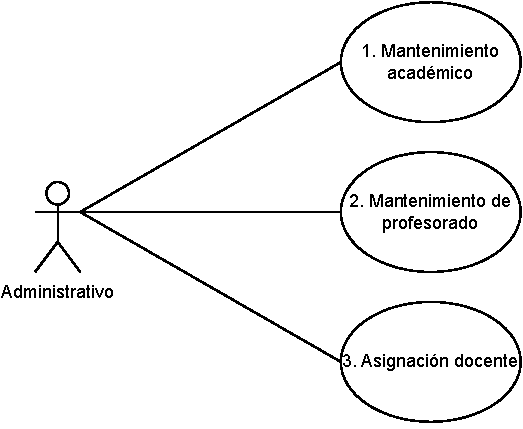
\includegraphics[scale=0.85]{../img/Anexos/Casos uso/Diagrama casos de uso 1.pdf}
	\caption{Diagrama de casos de uso general}
\end{figure}
\FloatBarrier

\subsubsection{1. Mantenimiento académico}
\begin{figure}[!h]
	\centering
	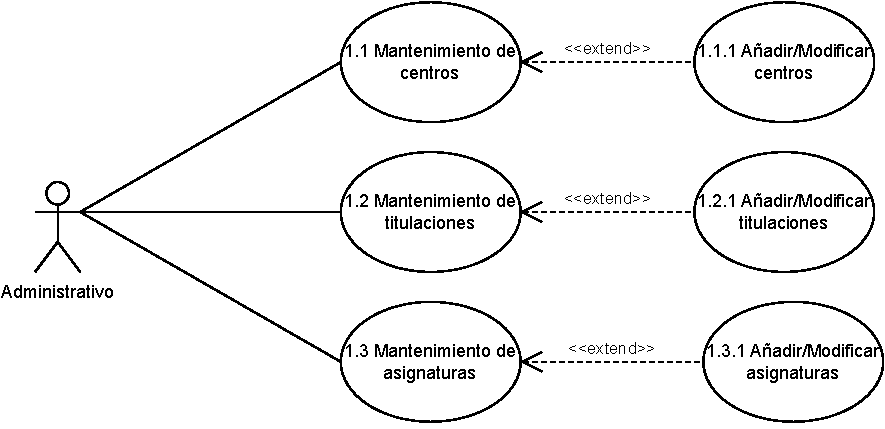
\includegraphics[scale=0.85]{../img/Anexos/Casos uso/Diagrama casos de uso 2.pdf}
	\caption{Diagrama de caso de uso - 1. Mantenimiento académico}
\end{figure}
\FloatBarrier

\begin{table}[p]
\label{table:CU-1}
	\centering
	\begin{tabularx}{\linewidth}{ p{0.21\columnwidth} p{0.71\columnwidth} }
		\toprule
		\textbf{CU-1}    & \textbf{Mantenimiento académico}\\
		\toprule
		\textbf{Versión}              & 1.0    \\
		\textbf{Autor}                & Ignacio Dávila García \\
		\textbf{Requisitos asociados} & \hyperref[itm:RF5]{RF-05}, \hyperref[itm:RF1]{RF-01}, \hyperref[itm:RF2]{RF-02} \\
		\textbf{Descripción}          & Un administrativo puede realizar labores de mantenimiento de los centros, titulaciones y asignaturas \\
		\textbf{Precondición}         & Tener iniciada sesión con una cuenta con permisos administrativos \\
		\textbf{Acciones}             &
		\begin{enumerate}
			\def\labelenumi{\arabic{enumi}.}
			\tightlist
			\item Seleccionar la opción <<Asignaturas>> del menú principal de la web.
			\item Se abre la ventana de mantenimiento de las asignaturas.
		\end{enumerate}\\
		\textbf{Postcondición}        & Ninguna \\
		\textbf{Excepciones}          & También es posible acceder la ventana de mantenimiento de centros y titulaciones seleccionando las opciones <<Centros>> (\hyperref[table:CU-1.1]{CU-1.1}) o <<Titulaciones>> (\hyperref[table:CU-1.2]{CU-1.2}) respectivamente. Si no se pulsa ninguna, se permanece en la ventana actual. \\
		\textbf{Importancia}          & Alta \\
		\bottomrule
	\end{tabularx}
	\caption{CU-1 Mantenimiento académico.}
\end{table}
\FloatBarrier

\begin{table}[p]
\label{table:CU-1.1}
	\centering
	\begin{tabularx}{\linewidth}{ p{0.21\columnwidth} p{0.71\columnwidth} }
		\toprule
		\textbf{CU-1.1}    & \textbf{Mantenimiento de centros}\\
		\toprule
		\textbf{Versión}              & 1.0    \\
		\textbf{Autor}                & Ignacio Dávila García \\
		\textbf{Requisitos asociados} & \hyperref[itm:RF5]{RF-05} \\
		\textbf{Descripción}          & Un administrativo puede realizar el mantenimiento de los centros \\
		\textbf{Precondición}         & Realizar el~\hyperref[table:CU-1]{CU-1} \\
		\textbf{Acciones}             &
		\begin{enumerate}
			\def\labelenumi{\arabic{enumi}.}
			\tightlist
			\item Se abre una ventana donde aparece una tabla con los centros creados desde donde se podrá realizar el mantenimiento.
		\end{enumerate}\\
		\textbf{Postcondición}        & Ninguna \\
		\textbf{Excepciones}          & Si se pulsa sobre el botón <<Nuevo>>, se accede a la creación de centros (\hyperref[table:CU-1.1.1]{CU-1.1.1}). Si se pulsa sobre el botón <<Modificar>> de un centro del listado, se accede a la ventana de modificación del centro. Por último, si se pulsa sobre el botón <<Eliminar>> de un centro el sistema pregunta si está seguro, y al pulsar en <<Sí>>, este se elimina produciendo un borrado en cascada de las titulaciones vinculadas. \\
		\textbf{Importancia}          & Alta \\
		\bottomrule
	\end{tabularx}
	\caption{CU-1.1 Mantenimiento de centros.}
\end{table}
\FloatBarrier

\begin{table}[p]
\label{table:CU-1.1.1}
	\centering
	\begin{tabularx}{\linewidth}{ p{0.21\columnwidth} p{0.71\columnwidth} }
		\toprule
		\textbf{CU-1.1.1}    & \textbf{Añadir/Modificar centros}\\
		\toprule
		\textbf{Versión}              & 1.0    \\
		\textbf{Autor}                & Ignacio Dávila García \\
		\textbf{Requisitos asociados} & \hyperref[itm:RF5]{RF-05} \\
		\textbf{Descripción}          & Un administrativo añade o modifica un nuevo centro \\
		\textbf{Precondición}         & Realizar el~\hyperref[table:CU-1.1]{CU-1.1} \\
		\textbf{Acciones}             &
		\begin{enumerate}
			\def\labelenumi{\arabic{enumi}.}
			\tightlist
			\item Se abre una ventana con un formulario vacío donde aparecen los campos de la tabla <<Centro>> de la figura \ref{er_cu1}, necesarios para crear un centro.
			\item Rellenar el formulario con los datos del centro que se desea añadir.
			\item Pulsar sobre el botón <<Añadir>>.
		\end{enumerate}\\
		\textbf{Postcondición}        & El centro queda añadido/modificado y el sistema lleva al usuario a la ventana de centros donde se puede ver el listado de todos los centros creados. \\
		\textbf{Excepciones}          & Se dejan campos vacíos o se introducen datos con un formato incorrecto. Otra forma de finalizar el caso de uso es la modificación. En este caso, se pulsa sobre el botón <<Modificar>> de un centro y se accede al mismo formulario con los campos rellenos. Finalmente se pulsa en el botón <<Modificar>> \\
		\textbf{Importancia}          & Alta \\
		\bottomrule
	\end{tabularx}
	\caption{CU-1.1.1 Añadir/Modificar centros.}
\end{table}
\FloatBarrier

\begin{table}[p]
\label{table:CU-1.2}
	\centering
	\begin{tabularx}{\linewidth}{ p{0.21\columnwidth} p{0.71\columnwidth} }
		\toprule
		\textbf{CU-1.2}    & \textbf{Mantenimiento de titulaciones}\\
		\toprule
		\textbf{Versión}              & 1.0    \\
		\textbf{Autor}                & Ignacio Dávila García \\
		\textbf{Requisitos asociados} & \hyperref[itm:RF1]{RF-01} \\
		\textbf{Descripción}          & Un administrativo puede realizar el mantenimiento de las titulaciones \\
		\textbf{Precondición}         & Realizar el~\hyperref[table:CU-1]{CU-1} \\
		\textbf{Acciones}             &
		\begin{enumerate}
			\def\labelenumi{\arabic{enumi}.}
			\tightlist
			\item Se abre una ventana donde aparece una tabla con las titulaciones creadas desde donde se podrá realizar el mantenimiento.
		\end{enumerate}\\
		\textbf{Postcondición}        & Ninguna \\
		\textbf{Excepciones}          & Si se pulsa sobre el botón <<Nuevo>>, se accede a la creación de titulaciones (\hyperref[table:CU-1.2.1]{CU-1.2.1}). Si se pulsa sobre el botón <<Modificar>> de una titulación de la lista se accede a la ventana de modificación. Por último, si se pulsa sobre el botón <<Eliminar>> de una titulación el sistema pregunta si está seguro, y al pulsar en <<Sí>>, esta se elimina produciendo un borrado en cascada de las asignaturas vinculadas. \\
		\textbf{Importancia}          & Alta \\
		\bottomrule
	\end{tabularx}
	\caption{CU-1.2 Mantenimiento de titulaciones.}
\end{table}
\FloatBarrier

\begin{table}[p]
\label{table:CU-1.2.1}
	\centering
	\begin{tabularx}{\linewidth}{ p{0.21\columnwidth} p{0.71\columnwidth} }
		\toprule
		\textbf{CU-1.2.1}    & \textbf{Añadir/Modificar titulaciones}\\
		\toprule
		\textbf{Versión}              & 1.0    \\
		\textbf{Autor}                & Ignacio Dávila García \\
		\textbf{Requisitos asociados} & \hyperref[itm:RF1]{RF-01} \\
		\textbf{Descripción}          & Un administrativo añade o modifica una titulación \\
		\textbf{Precondición}         & Realizar el~\hyperref[table:CU-1.2]{CU-1.2} y tener algún centro creado \\
		\textbf{Acciones}             &
		\begin{enumerate}
			\def\labelenumi{\arabic{enumi}.}
			\tightlist
			\item Se abre una ventana con un formulario vacío donde aparecen los campos de la tabla <<Titulación>> de la figura \ref{er_cu1}, necesarios para crear una titulación. También aparece el campo <<Centro>> para seleccionar el centro al que pertenece.
			\item Rellenar el formulario con los datos de la titulación que se desea añadir.
			\item Pulsar sobre el botón <<Añadir>>.
		\end{enumerate}\\
		\textbf{Postcondición}        & La titulación queda añadida/modificada y el sistema lleva al usuario a la ventana de titulaciones donde se puede ver el listado de todos las titulaciones añadidas. \\
		\textbf{Excepciones}          & Se dejan campos vacíos o se introducen datos con un formato incorrecto. Otra forma de finalizar el caso de uso es la modificación. En este caso, se pulsa sobre el botón <<Modificar>> de una titulación de la tabla y se accede al mismo formulario, pero con los campos rellenos. Finalmente se pulsa en el botón <<Modificar>> y la titulación queda modificada. \\
		\textbf{Importancia}          & Alta \\
		\bottomrule
	\end{tabularx}
	\caption{CU-1.2.1 Añadir/Modificar centros.}
\end{table}
\FloatBarrier

\begin{table}[p]
\label{table:CU-1.3}
	\centering
	\begin{tabularx}{\linewidth}{ p{0.21\columnwidth} p{0.71\columnwidth} }
		\toprule
		\textbf{CU-1.3}    & \textbf{Mantenimiento de asignaturas}\\
		\toprule
		\textbf{Versión}              & 1.0    \\
		\textbf{Autor}                & Ignacio Dávila García \\
		\textbf{Requisitos asociados} & \hyperref[itm:RF2]{RF-02} \\
		\textbf{Descripción}          & Un administrativo puede realizar el mantenimiento de asignaturas \\
		\textbf{Precondición}         & Realizar el~\hyperref[table:CU-1]{CU-1} \\
		\textbf{Acciones}             &
		\begin{enumerate}
			\def\labelenumi{\arabic{enumi}.}
			\tightlist
			\item Se abre una ventana donde aparece una tabla con las asignaturas creadas desde donde se podrá realizar el mantenimiento.
		\end{enumerate}\\
		\textbf{Postcondición}        & Ninguna \\
		\textbf{Excepciones}          & Si se pulsa sobre el botón <<Nuevo>>, se accede a la creación de asignaturas (\hyperref[table:CU-1.3.1]{CU-1.3.1}). Si se pulsa sobre el botón <<Modificar>> de una asignaturas de la lista se accede a la ventana de modificación. Por último, si se pulsa sobre el botón <<Eliminar>> de una asignatura el sistema pregunta si está seguro, y al pulsar en <<Sí>> esta se elimina. \\
		\textbf{Importancia}          & Alta \\
		\bottomrule
	\end{tabularx}
	\caption{CU-1.3 Mantenimiento de asignaturas.}
\end{table}
\FloatBarrier

\begin{table}[p]
\label{table:CU-1.3.1}
	\centering
	\begin{tabularx}{\linewidth}{ p{0.21\columnwidth} p{0.71\columnwidth} }
		\toprule
		\textbf{CU-1.3.1}    & \textbf{Añadir/Modificar asignaturas}\\
		\toprule
		\textbf{Versión}              & 1.0    \\
		\textbf{Autor}                & Ignacio Dávila García \\
		\textbf{Requisitos asociados} & \hyperref[itm:RF2]{RF-02} \\
		\textbf{Descripción}          & Un administrativo añade o modifica una asignatura \\
		\textbf{Precondición}         & Realizar el~\hyperref[table:CU-1.3]{CU-1.3} y tener alguna titulación creada \\
		\textbf{Acciones}             &
		\begin{enumerate}
			\def\labelenumi{\arabic{enumi}.}
			\tightlist
			\item Se abre una ventana con un formulario vacío donde aparecen los campos de la tabla <<Asignatura>> de la figura \ref{er_cu1}, necesarios para crear una asignatura. También se debe indicar la titulación a la que pertenece y rellenar el campo <<Abreviatura>> que permite la selección múltiple de abreviaturas separadas por comas. Las abreviaturas existentes aparecen al escribir y se pueden seleccionar. Si se escribe una nueva se almacena.
			\item Rellenar el formulario con los datos de la asignatura que se desea añadir.
			\item Pulsar sobre el botón <<Añadir>>.
		\end{enumerate}\\
		\textbf{Postcondición}        & La asignatura queda añadida/modificada y el sistema lleva al usuario a la ventana de asignaturas donde se puede ver el listado de todos las asignaturas añadidas. \\
		\textbf{Excepciones}          & Se dejan campos vacíos, se introducen datos con un formato incorrecto o se introduce una id existente. Otra forma de finalizar el caso de uso es la modificación. En este caso, se pulsa sobre el botón <<Modificar>> de una asignatura de la tabla y se accede al mismo formulario, pero con los campos rellenos. Finalmente se pulsa en el botón <<Modificar>> y la asignatura queda modificada. \\
		\textbf{Importancia}          & Alta \\
		\bottomrule
	\end{tabularx}
	\caption{CU-1.3.1 Añadir/Modificar asignaturas.}
\end{table}
\FloatBarrier

\begin{figure}[!h]
	\centering
	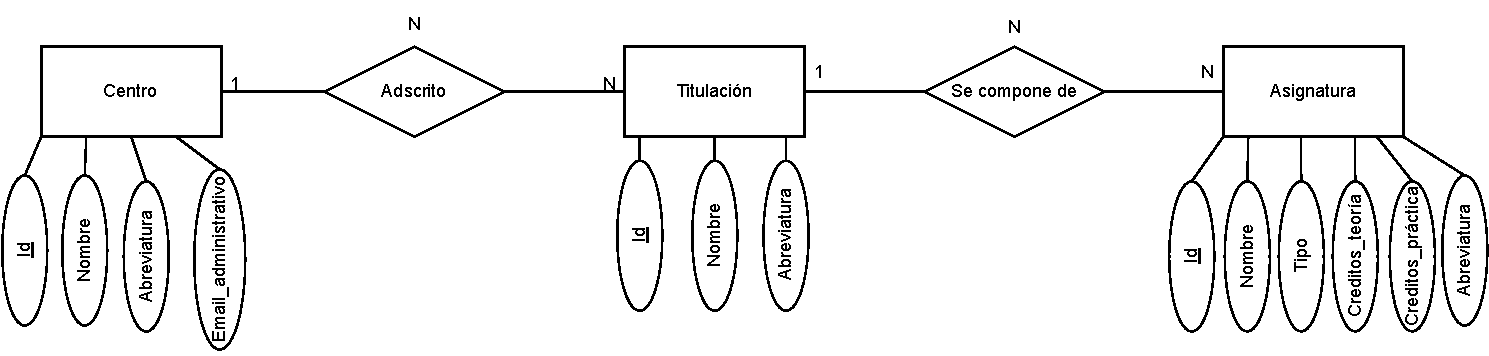
\includegraphics[scale=0.75]{../img/Anexos/Casos uso/Vistas ER/Diagrama E-R CU 1.pdf}
	\caption{Vista diagrama entidad relación para el CU-1}
	\label{er_cu1}
\end{figure}
\FloatBarrier

\newpage
\subsubsection{2. Mantenimiento de profesorado}
\begin{figure}[!h]
	\centering
	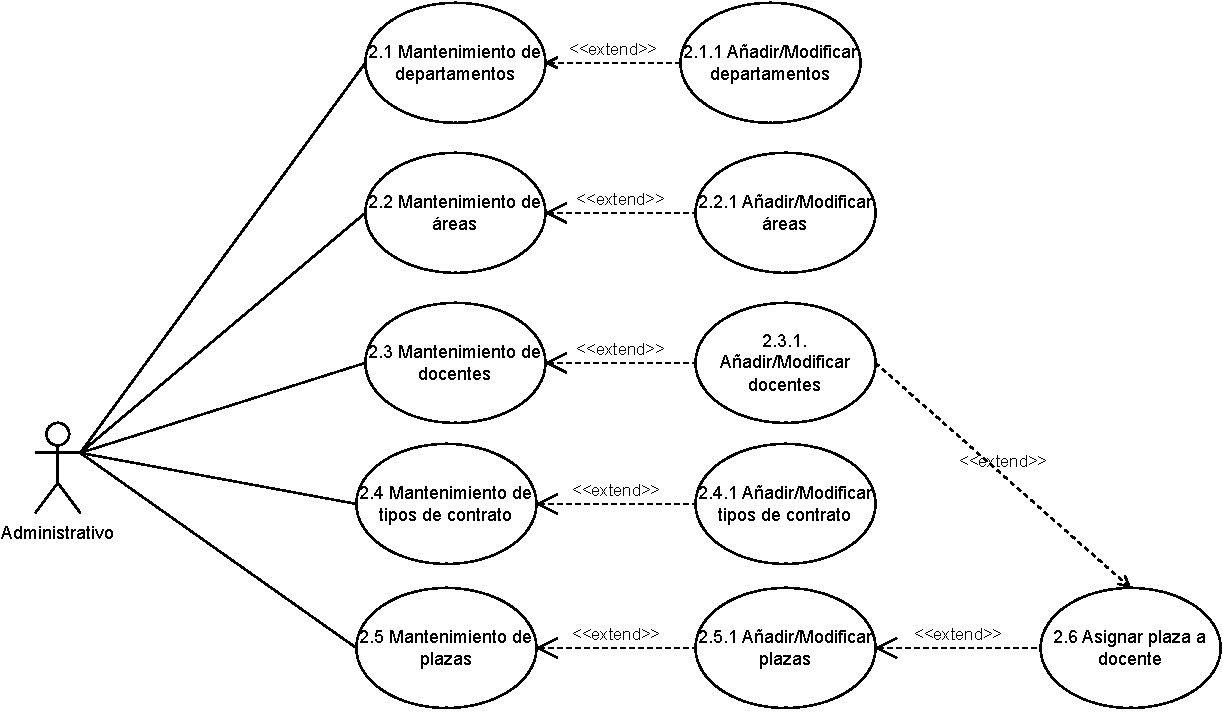
\includegraphics[scale=0.75]{../img/Anexos/Casos uso/Diagrama casos de uso 3.pdf}
	\caption{Diagrama de caso de uso - 2. Mantenimiento de profesorado}
\end{figure}
\FloatBarrier

\begin{table}[p]
\label{table:CU-2}
	\centering
	\begin{tabularx}{\linewidth}{ p{0.21\columnwidth} p{0.71\columnwidth} }
		\toprule
		\textbf{CU-2}    & \textbf{Mantenimiento de profesorado}\\
		\toprule
		\textbf{Versión}              & 1.0    \\
		\textbf{Autor}                & Ignacio Dávila García \\
		\textbf{Requisitos asociados} & \hyperref[itm:RF4]{RF-04}, \hyperref[itm:RF7]{RF-07}, \hyperref[itm:RF8]{RF-08}, \hyperref[itm:RF9]{RF-09}, \hyperref[itm:RF10]{RF-10} \\
		\textbf{Descripción}          & Un administrativo puede realizar labores de mantenimiento de los docentes, tipos de contrato, departamentos, áreas y plazas. Además, un administrativo puede asignar una plaza a un docente. \\
		\textbf{Precondición}         & Tener iniciada sesión con una cuenta con permisos administrativos \\
		\textbf{Acciones}             &
		\begin{enumerate}
			\def\labelenumi{\arabic{enumi}.}
			\tightlist
			\item Seleccionar la opción <<Plazas>> del menú principal de la web.
			\item Se abre la ventana de mantenimiento de plazas.
		\end{enumerate}\\
		\textbf{Postcondición}        & El sistema lleva al usuario a la ventana de la opción pulsada. \\
		\textbf{Excepciones}          & Otras opciones que se pueden seleccionar son <<Docentes>> (\hyperref[table:CU-2.3]{CU-2.3}), <<Contratos>> (\hyperref[table:CU-2.4]{CU-2.4}), <<Departamentos>> (\hyperref[table:CU-2.1]{CU-2.1}) o <<Áreas>> (\hyperref[table:CU-2.2]{CU-2.2}). Al seleccionar alguna de estas opciones el sistema lleva al usuario a la ventana de mantenimiento de la opción elegida.  \\
		\textbf{Importancia}          & Alta \\
		\bottomrule
	\end{tabularx}
	\caption{CU-2 Mantenimiento de profesorado.}
\end{table}
\FloatBarrier

\begin{table}[p]
\label{table:CU-2.1}
	\centering
	\begin{tabularx}{\linewidth}{ p{0.21\columnwidth} p{0.71\columnwidth} }
		\toprule
		\textbf{CU-2.1}    & \textbf{Mantenimiento de departamentos}\\
		\toprule
		\textbf{Versión}              & 1.0    \\
		\textbf{Autor}                & Ignacio Dávila García \\
		\textbf{Requisitos asociados} & \hyperref[itm:RF10]{RF-10} \\
		\textbf{Descripción}          & Un administrativo puede realizar el mantenimiento de departamentos \\
		\textbf{Precondición}         & Realizar el~\hyperref[table:CU-2]{CU-2} \\
		\textbf{Acciones}             &
		\begin{enumerate}
			\def\labelenumi{\arabic{enumi}.}
			\tightlist
			\item Se abre una ventana donde aparece una tabla con los departamentos creados desde donde se podrá realizar el mantenimiento.
		\end{enumerate}\\
		\textbf{Postcondición}        & Ninguna \\
		\textbf{Excepciones}          & Si se pulsa sobre el botón <<Nuevo>>, se accede a la creación de departamentos (\hyperref[table:CU-2.1.1]{CU-2.1.1}). Si se pulsa sobre el botón <<Modificar>> de un departamento de la lista, se accede a la ventana de modificación. Por último, si se pulsa sobre el botón <<Eliminar>> de un departamento el sistema pregunta si está seguro, y al pulsar en <<Sí>>, este se elimina produciendo un borrado en cascada de las áreas asociadas. \\
		\textbf{Importancia}          & Alta \\
		\bottomrule
	\end{tabularx}
	\caption{CU-2.1 Mantenimiento de departamentos.}
\end{table}
\FloatBarrier

\begin{table}[p]
\label{table:CU-2.1.1}
	\centering
	\begin{tabularx}{\linewidth}{ p{0.21\columnwidth} p{0.71\columnwidth} }
		\toprule
		\textbf{CU-2.1.1}    & \textbf{Añadir/Modificar departamentos}\\
		\toprule
		\textbf{Versión}              & 1.0    \\
		\textbf{Autor}                & Ignacio Dávila García \\
		\textbf{Requisitos asociados} & \hyperref[itm:RF10]{RF-10} \\
		\textbf{Descripción}          & Un administrativo añade o modifica un departamento \\
		\textbf{Precondición}         & Realizar el~\hyperref[table:CU-2.1]{CU-2.1} \\
		\textbf{Acciones}             &
		\begin{enumerate}
			\def\labelenumi{\arabic{enumi}.}
			\tightlist
			\item Se abre una ventana con un formulario vacío donde aparecen los campos de la tabla <<Departamento>> de la figura \ref{er_cu2}, necesarios para crear un departamento.
			\item Rellenar el formulario con los datos del departamento que se desea añadir.
			\item Pulsar sobre el botón <<Añadir>>.
		\end{enumerate}\\
		\textbf{Postcondición}        & El departamento queda añadido/modificado y el sistema lleva al usuario a la ventana de departamentos donde se puede ver el listado de todos los departamento añadidos. \\
		\textbf{Excepciones}          & Se dejan campos vacíos o se introducen datos con un formato incorrecto. Otra forma de finalizar el caso de uso es la modificación. En este caso, se pulsa sobre el botón <<Modificar>> de un departamento de la tabla y se accede al mismo formulario, pero con los campos rellenos. Finalmente se pulsa en el botón <<Modificar>> y el departamento queda modificado. \\
		\textbf{Importancia}          & Alta \\
		\bottomrule
	\end{tabularx}
	\caption{CU-2.1.1 Añadir/Modificar departamentos.}
\end{table}
\FloatBarrier

\begin{table}[p]
\label{table:CU-2.2}
	\centering
	\begin{tabularx}{\linewidth}{ p{0.21\columnwidth} p{0.71\columnwidth} }
		\toprule
		\textbf{CU-2.2}    & \textbf{Mantenimiento de áreas}\\
		\toprule
		\textbf{Versión}              & 1.0    \\
		\textbf{Autor}                & Ignacio Dávila García \\
		\textbf{Requisitos asociados} & \hyperref[itm:RF9]{RF-09} \\
		\textbf{Descripción}          & Un administrativo puede realizar el mantenimiento de áreas \\
		\textbf{Precondición}         & Realizar el~\hyperref[table:CU-2]{CU-2} \\
		\textbf{Acciones}             &
		\begin{enumerate}
			\def\labelenumi{\arabic{enumi}.}
			\tightlist
			\item Se abre una ventana donde aparece una tabla con las áreas creadas desde donde se podrá realizar el mantenimiento.
		\end{enumerate}\\
		\textbf{Postcondición}        & Ninguna \\
		\textbf{Excepciones}          & Si se pulsa sobre el botón <<Nuevo>>, se accede a la creación de áreas (\hyperref[table:CU-2.2.1]{CU-2.2.1}). Si se pulsa sobre el botón <<Modificar>> de un área de la lista, se accede a la ventana de modificación. Por último, si se pulsa sobre el botón <<Eliminar>> de un área el sistema pregunta si está seguro, y al pulsar en <<Sí>>, esta se elimina produciendo un borrado en cascada de las plazas asociadas. \\
		\textbf{Importancia}          & Alta \\
		\bottomrule
	\end{tabularx}
	\caption{CU-2.2 Mantenimiento de áreas.}
\end{table}
\FloatBarrier

\begin{table}[p]
\label{table:CU-2.2.1}
	\centering
	\begin{tabularx}{\linewidth}{ p{0.21\columnwidth} p{0.71\columnwidth} }
		\toprule
		\textbf{CU-2.2.1}    & \textbf{Añadir/Modificar áreas}\\
		\toprule
		\textbf{Versión}              & 1.0    \\
		\textbf{Autor}                & Ignacio Dávila García \\
		\textbf{Requisitos asociados} & \hyperref[itm:RF9]{RF-09} \\
		\textbf{Descripción}          & Un administrativo añade o modifica un área \\
		\textbf{Precondición}         & Realizar el~\hyperref[table:CU-2]{CU-2} y tener algún departamento creado \\
		\textbf{Acciones}             &
		\begin{enumerate}
			\def\labelenumi{\arabic{enumi}.}
			\tightlist
			\item Se abre una ventana con un formulario vacío donde aparecen los campos de la tabla <<Área>> de la figura \ref{er_cu2}, necesarios para crear un área. También se debe indicar el departamento al que pertenece el área.
			\item Rellenar el formulario con los datos del área que se desea añadir.
			\item Pulsar sobre el botón <<Añadir>>.
		\end{enumerate}\\
		\textbf{Postcondición}        & El área queda añadido/modificado y el sistema lleva al usuario a la ventana de áreas donde se puede ver el listado de todas las áreas añadidas. \\
		\textbf{Excepciones}          & Se dejan campos vacíos o se introducen datos con un formato incorrecto. Otra forma de finalizar el caso de uso es la modificación. En este caso, se pulsa sobre el botón <<Modificar>> de un área de la tabla y se accede al mismo formulario, pero con los campos rellenos. Finalmente se pulsa en el botón <<Modificar>> y el área queda modificada. \\
		\textbf{Importancia}          & Alta \\
		\bottomrule
	\end{tabularx}
	\caption{CU-2.2.1 Añadir/Modificar áreas.}
\end{table}
\FloatBarrier

\begin{table}[p]
\label{table:CU-2.3}
	\centering
	\begin{tabularx}{\linewidth}{ p{0.21\columnwidth} p{0.71\columnwidth} }
		\toprule
		\textbf{CU-2.3}    & \textbf{Mantenimiento de docentes}\\
		\toprule
		\textbf{Versión}              & 1.0    \\
		\textbf{Autor}                & Ignacio Dávila García \\
		\textbf{Requisitos asociados} & \hyperref[itm:RF4]{RF-04} \\
		\textbf{Descripción}          & Un administrativo puede realizar el mantenimiento de docentes \\
		\textbf{Precondición}         & Realizar el~\hyperref[table:CU-2]{CU-2} \\
		\textbf{Acciones}             &
		\begin{enumerate}
			\def\labelenumi{\arabic{enumi}.}
			\tightlist
			\item Seleccionar la opción <<Docentes>> del menú principal de la web.
			\item Se abre una ventana donde aparece una tabla con los docentes creados desde donde se podrá realizar el mantenimiento.
		\end{enumerate}\\
		\textbf{Postcondición}        & Ninguna \\
		\textbf{Excepciones}          & Si se pulsa sobre el botón <<Nuevo>>, se accede a la creación de docentes (\hyperref[table:CU-2.3.1]{CU-2.3.1}). Si se pulsa sobre el botón <<Modificar>> de un docente de la lista, se accede a la ventana de modificación. Por último, si se pulsa sobre el botón <<Eliminar>> de un docente el sistema pregunta si está seguro, y al pulsar en <<Sí>>, este se elimina. \\
		\textbf{Importancia}          & Alta \\
		\bottomrule
	\end{tabularx}
	\caption{CU-2.3 Mantenimiento de docentes.}
\end{table}
\FloatBarrier

\begin{table}[p]
\label{table:CU-2.3.1}
	\centering
	\begin{tabularx}{\linewidth}{ p{0.21\columnwidth} p{0.71\columnwidth} }
		\toprule
		\textbf{CU-2.3.1}    & \textbf{Añadir/Modificar docentes}\\
		\toprule
		\textbf{Versión}              & 1.0    \\
		\textbf{Autor}                & Ignacio Dávila García \\
		\textbf{Requisitos asociados} & \hyperref[itm:RF4]{RF-04} \\
		\textbf{Descripción}          & Un administrativo añade o modifica un docente \\
		\textbf{Precondición}         & Realizar el~\hyperref[table:CU-2.3]{CU-2.3} \\
		\textbf{Acciones}             &
		\begin{enumerate}
			\def\labelenumi{\arabic{enumi}.}
			\tightlist
			\item Se abre una ventana con un formulario vacío donde aparecen los campos de la tabla <<Docente>> de la figura \ref{er_cu2}, necesarios para crear un docente.
			\item Rellenar el formulario con los datos del docente que se desea añadir.
			\item Pulsar sobre el botón <<Añadir>>.
		\end{enumerate}\\
		\textbf{Postcondición}        & El docente queda añadido/modificado y el sistema lleva al usuario a la ventana de docentes donde se puede ver el listado de todos los docentes añadidos. \\
		\textbf{Excepciones}          & Se dejan campos vacíos o se introducen datos con un formato incorrecto. Otra forma de finalizar el caso de uso es la modificación. En este caso, se pulsa sobre el botón <<Modificar>> de un docente de la tabla y se accede al mismo formulario, pero con los campos rellenos. Finalmente se pulsa en el botón <<Modificar>> y el docente queda modificado. \\
		\textbf{Importancia}          & Alta \\
		\bottomrule
	\end{tabularx}
	\caption{CU-2.3.1 Añadir/Modificar docentes.}
\end{table}
\FloatBarrier

\begin{table}[p]
\label{table:CU-2.4}
	\centering
	\begin{tabularx}{\linewidth}{ p{0.21\columnwidth} p{0.71\columnwidth} }
		\toprule
		\textbf{CU-2.4}    & \textbf{Mantenimiento de tipos de contrato}\\
		\toprule
		\textbf{Versión}              & 1.0    \\
		\textbf{Autor}                & Ignacio Dávila García \\
		\textbf{Requisitos asociados} & \hyperref[itm:RF8]{RF-08} \\
		\textbf{Descripción}          & Un administrativo puede realizar el mantenimiento de tipos de contrato \\
		\textbf{Precondición}         & Realizar el~\hyperref[table:CU-2]{CU-2} \\
		\textbf{Acciones}             &
		\begin{enumerate}
			\def\labelenumi{\arabic{enumi}.}
			\tightlist
			\item Seleccionar la opción <<Contratos>> del menú principal de la web.
			\item Se abre una ventana donde aparece una tabla con los tipos de contrato creados desde donde se podrá realizar el mantenimiento.
		\end{enumerate}\\
		\textbf{Postcondición}        & Ninguna \\
		\textbf{Excepciones}          & Si se pulsa sobre el botón <<Nuevo>>, se accede a la creación de un nuevo tipo de contrato (\hyperref[table:CU-2.4.1]{CU-2.4.1}). Si se pulsa sobre el botón <<Modificar>> de un tipo de contrato de la lista, se accede a la ventana de modificación. Por último, si se pulsa sobre el botón <<Eliminar>> de un tipo de contrato el sistema pregunta si está seguro, y al pulsar en <<Sí>>, este se elimina. \\
		\textbf{Importancia}          & Alta \\
		\bottomrule
	\end{tabularx}
	\caption{CU-2.4 Mantenimiento de tipos de contrato.}
\end{table}
\FloatBarrier

\begin{table}[p]
\label{table:CU-2.4.1}
	\centering
	\begin{tabularx}{\linewidth}{ p{0.21\columnwidth} p{0.71\columnwidth} }
		\toprule
		\textbf{CU-2.4.1}    & \textbf{Añadir/Modificar tipos de contrato}\\
		\toprule
		\textbf{Versión}              & 1.0    \\
		\textbf{Autor}                & Ignacio Dávila García \\
		\textbf{Requisitos asociados} & \hyperref[itm:RF8]{RF-08} \\
		\textbf{Descripción}          & Un administrativo añade o modifica un docente \\
		\textbf{Precondición}         & Realizar el~\hyperref[table:CU-2.4]{CU-2.4} \\
		\textbf{Acciones}             &
		\begin{enumerate}
			\def\labelenumi{\arabic{enumi}.}
			\tightlist
			\item Se abre una ventana con un formulario vacío donde aparecen los campos de la tabla <<Tipo Contrato>> de la figura~\ref{er_cu2}, necesarios para crear un tipo de contrato.
			\item Rellenar el formulario con los datos del tipo de contrato que se desea añadir.
			\item Pulsar sobre el botón <<Añadir>>.
		\end{enumerate}\\
		\textbf{Postcondición}        & El tipo de contrato queda añadido/modificado y el sistema lleva al usuario a la ventana de tipos de contrato donde se puede ver el listado de todos los tipos de contrato añadidos. \\
		\textbf{Excepciones}          & Se dejan campos vacíos o se introducen datos con un formato incorrecto. Otra forma de finalizar el caso de uso es la modificación. En este caso, se pulsa sobre el botón <<Modificar>> de un tipo de contrato de la tabla y se accede al mismo formulario, pero con los campos rellenos. Finalmente se pulsa en el botón <<Modificar>> y el tipo de contrato queda modificado. \\
		\textbf{Importancia}          & Alta \\
		\bottomrule
	\end{tabularx}
	\caption{CU-2.4.1 Añadir/Modificar tipos de contrato.}
\end{table}
\FloatBarrier

\begin{table}[p]
\label{table:CU-2.5}
	\centering
	\begin{tabularx}{\linewidth}{ p{0.21\columnwidth} p{0.71\columnwidth} }
		\toprule
		\textbf{CU-2.5}    & \textbf{Mantenimiento de plazas}\\
		\toprule
		\textbf{Versión}              & 1.0    \\
		\textbf{Autor}                & Ignacio Dávila García \\
		\textbf{Requisitos asociados} & \hyperref[itm:RF7]{RF-07} \\
		\textbf{Descripción}          & Un administrativo puede realizar el mantenimiento de plazas \\
		\textbf{Precondición}         & Realizar el~\hyperref[table:CU-2]{CU-2} \\
		\textbf{Acciones}             &
		\begin{enumerate}
			\def\labelenumi{\arabic{enumi}.}
			\tightlist
			\item Se abre una ventana donde aparece una tabla con las plazas creadas desde donde se podrá realizar el mantenimiento.
		\end{enumerate}\\
		\textbf{Postcondición}        & Ninguna \\
		\textbf{Excepciones}          & Si se pulsa sobre el botón <<Nuevo>>, se accede a la creación de una plaza (\hyperref[table:CU-2.5.1]{CU-2.5.1}). Si se pulsa sobre el botón <<Modificar>> de una plaza de la lista, se accede a la ventana de modificación. Desde la ventana de modificación también se puede acceder al~\hyperref[table:CU-2.6]{CU-2.6} de asignar una plaza a un docente. Por último, si se pulsa sobre el botón <<Eliminar>> de una plaza el sistema pregunta si está seguro, y al pulsar en <<Sí>>, esta se elimina. \\
		\textbf{Importancia}          & Alta \\
		\bottomrule
	\end{tabularx}
	\caption{CU-2.5 Mantenimiento de plazas.}
\end{table}
\FloatBarrier

\begin{table}[p]
	\label{table:CU-2.5.1}
	\centering
	\begin{tabularx}{\linewidth}{ p{0.21\columnwidth} p{0.71\columnwidth} }
		\toprule
		\textbf{CU-2.5.1}    & \textbf{Añadir/Modificar plazas}\\
		\toprule
		\textbf{Versión}              & 1.0    \\
		\textbf{Autor}                & Ignacio Dávila García \\
		\textbf{Requisitos asociados} & \hyperref[itm:RF7]{RF-07} \\
		\textbf{Descripción}          & Un administrativo añade o modifica una plaza \\
		\textbf{Precondición}         & Realizar el~\hyperref[table:CU-2.5]{CU-2.5} y tener algún área y tipo de contrato creados \\
		\textbf{Acciones}             &
		\begin{enumerate}
			\def\labelenumi{\arabic{enumi}.}
			\tightlist
			\item Se abre una ventana con un formulario vacío donde aparecen los campos de la tabla <<Plaza>> de la figura~\ref{er_cu2}, necesarios para crear una plaza. También se debe indicar el tipo de contrato y se puede asignar la plaza a un docente (\hyperref[table:CU-2.6]{CU-2.6}).
			\item Rellenar el formulario con los datos de la plaza que se desea añadir.
			\item Pulsar sobre el botón <<Añadir>>.
		\end{enumerate}\\
		\textbf{Postcondición}        & La plaza queda añadida/modificada y el sistema lleva al usuario a la ventana de plazas donde se puede ver el listado de todas las plazas añadidas. \\
		\textbf{Excepciones}          & Se dejan campos vacíos o se introducen datos con un formato incorrecto. Otra forma de finalizar el caso de uso es la modificación. En este caso, se pulsa sobre el botón <<Modificar>> de una plaza de la tabla y se accede al mismo formulario, pero con los campos rellenos. Finalmente se pulsa en el botón <<Modificar>> y la plaza queda modificada. \\
		\textbf{Importancia}          & Alta \\
		\bottomrule
	\end{tabularx}
	\caption{CU-2.5.1 Añadir/Modificar plazas.}
\end{table}
\FloatBarrier

\begin{table}[p]
\label{table:CU-2.6}
	\centering
	\begin{tabularx}{\linewidth}{ p{0.21\columnwidth} p{0.71\columnwidth} }
		\toprule
		\textbf{CU-2.6}    & \textbf{Asignar plaza a docente}\\
		\toprule
		\textbf{Versión}              & 1.0    \\
		\textbf{Autor}                & Ignacio Dávila García \\
		\textbf{Requisitos asociados} & \hyperref[itm:RF7]{RF-07}, \hyperref[itm:RF12]{RF-12} \\
		\textbf{Descripción}          & Un administrativo puede asignar una plaza a un docente. Este caso de uso es una extensión del \hyperref[table:CU-2.5.1]{CU-2.5.1}, ya que la asignación de la plaza a un docente se realiza en la creación o modificación de la misma \\
		\textbf{Precondición}         & Realizar el~\hyperref[table:CU-2.5]{CU-2.5} y tener creado un docente \\
		\textbf{Acciones}             &
		\begin{enumerate}
			\def\labelenumi{\arabic{enumi}.}
			\tightlist
			\item Si la plaza que se desea asignar ya está creada, pulsar en el botón <<Modificar>> de la fila de la tabla que corresponde a la plaza.
			\item Se abre una ventana con un formulario que tendrá los campos de la tabla <<Plaza>> de la figura \ref{er_cu2} rellenos. En el campo llamado <<Docente>>, se podrá seleccionar el docente al que se quiere asignar la plaza desde un seleccionable con búsqueda.
		\end{enumerate}\\
		\textbf{Postcondición}        & La plaza queda asignada al docente seleccionado y el sistema lleva al usuario a la vista del mantenimiento de plazas. \\
		\textbf{Excepciones}          & La asignación se puede realizar a la hora de crear una plaza. Para ello, se debe pulsar en el botón <<Nuevo>> desde la ventana de mantenimiento de plazas y se abrirá una ventana con el mismo formulario, pero vacío. Después de rellenar los datos, se pulsa en el botón <<Añadir>> y la plaza queda creada y asignada.
		Si el docente al que se desea vincular la plaza todavía no está creado, este se puede crear pulsando sobre el botón <<Nuevo docente>> que se encuentra dentro del formulario. Pulsar el botón hará que se abra una ventana flotante que cubre el \hyperref[table:CU-2.3.1]{CU-2.3.1} para añadir un nuevo docente.\\
		\textbf{Importancia}          & Alta \\
		\bottomrule
	\end{tabularx}
	\caption{CU-2.6 Asignar plaza a docente.}
\end{table}
\FloatBarrier

\begin{figure}[!h]
	\centering
	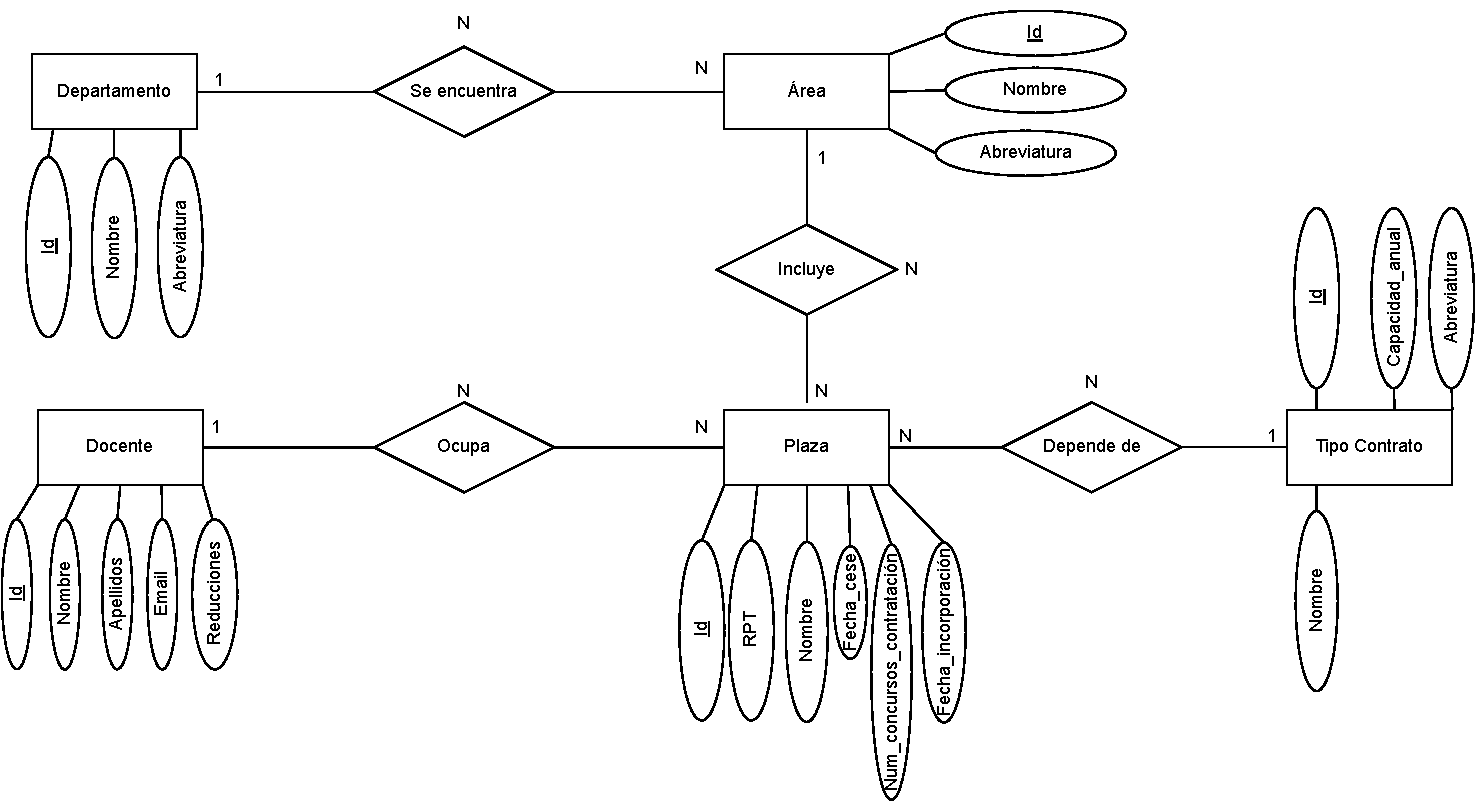
\includegraphics[scale=0.7]{../img/Anexos/Casos uso/Vistas ER/Diagrama E-R CU 2.pdf}
	\caption{Vista diagrama entidad relación para el CU-2}\label{er_cu2}
\end{figure}
\FloatBarrier

\newpage
\subsubsection{3. Asignación docente}
\begin{figure}[!h]
	\centering
	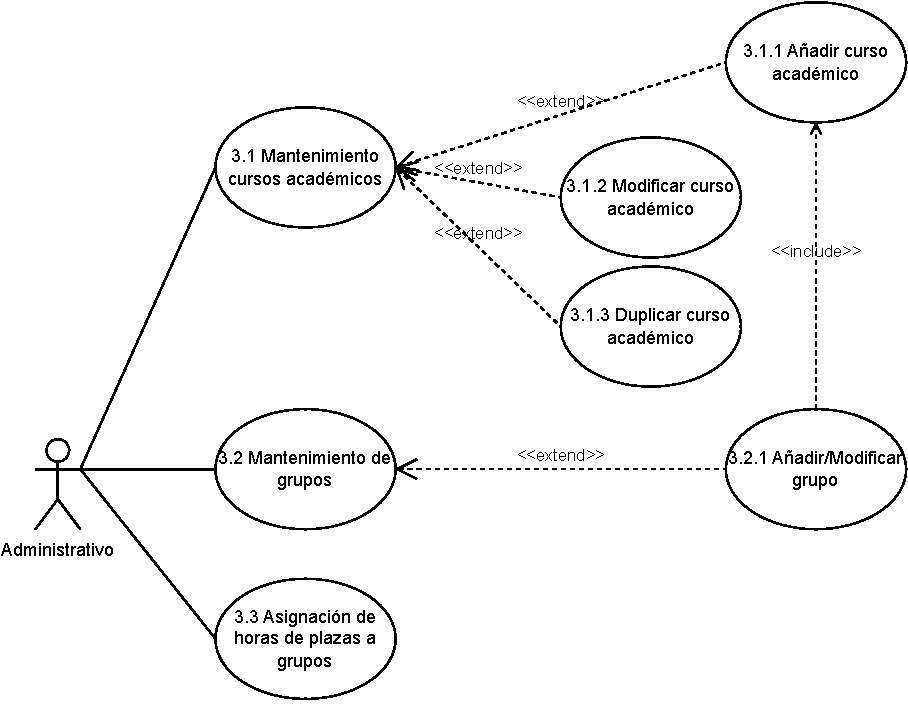
\includegraphics[scale=0.9]{../img/Anexos/Casos uso/Diagrama casos de uso 4.pdf}
	\caption{Diagrama de caso de uso - 3. Asignación docente}
\end{figure}
\FloatBarrier

\begin{table}[p]
\label{table:CU-3}
	\centering
	\begin{tabularx}{\linewidth}{ p{0.21\columnwidth} p{0.71\columnwidth} }
		\toprule
		\textbf{CU-3}    & \textbf{Asignación docente}\\
		\toprule
		\textbf{Versión}              & 1.0    \\
		\textbf{Autor}                & Ignacio Dávila García \\
		\textbf{Requisitos asociados} & \hyperref[itm:RF6]{RF-06}, \hyperref[itm:RF7]{RF-07}, \hyperref[itm:RF8]{RF-08}, \hyperref[itm:RF9]{RF-09}, \hyperref[itm:RF10]{RF-10} \\
		\textbf{Descripción}          & Un administrativo puede realizar las labores de mantenimiento de cursos y grupos, además de las asignaciones de horas de plazas a grupos \\
		\textbf{Precondición}         & Tener iniciada sesión con una cuenta con permisos administrativos \\
		\textbf{Acciones}             &
		\begin{enumerate}
			\def\labelenumi{\arabic{enumi}.}
			\tightlist
			\item Seleccionar la opción del menú <<Grupos>> para realizar el mantenimiento de los mismos.
			\item Se abre la ventana de mantenimiento de cursos.
		\end{enumerate}\\
		\textbf{Postcondición}        & El sistema lleva al usuario a la ventana de la opción pulsada. \\
		\textbf{Excepciones}          & Otras posibilidades del caso de uso son el mantenimiento de cursos académicos, que se puede realizar seleccionando la opción del menú <<Cursos>> (\hyperref[table:CU-3.1]{CU-3.1}) y la asignación de horas de una plaza a un grupo, que se puede realizar seleccionando la opción <<Horas>> (\hyperref[table:CU-3.3]{CU-3.3}). \\
		\textbf{Importancia}          & Alta \\
		\bottomrule
	\end{tabularx}
	\caption{CU-3 Asignación docente.}
\end{table}
\FloatBarrier

\begin{table}[p]
\label{table:CU-3.1}
	\centering
	\begin{tabularx}{\linewidth}{ p{0.21\columnwidth} p{0.71\columnwidth} }
		\toprule
		\textbf{CU-3.1}    & \textbf{Mantenimiento cursos académicos}\\
		\toprule
		\textbf{Versión}              & 1.0    \\
		\textbf{Autor}                & Ignacio Dávila García \\
		\textbf{Requisitos asociados} & \hyperref[itm:RF6]{RF-06} \\
		\textbf{Descripción}          & Un administrativo puede realizar el mantenimiento de los cursos académicos \\
		\textbf{Precondición}         & Realizar el~\hyperref[table:CU-3]{CU-3} \\
		\textbf{Acciones}             &
		\begin{enumerate}
			\def\labelenumi{\arabic{enumi}.}
			\tightlist
			\item Seleccionar la opción <<Cursos>> del menú principal de la web.
			\item Se abre una ventana donde aparece una tabla con los cursos creados desde donde se podrá realizar el mantenimiento.
		\end{enumerate}\\
		\textbf{Postcondición}        & Ninguna \\
		\textbf{Excepciones}          & Si se pulsa sobre el botón <<Nuevo>>, se accede a la creación de un curso (\hyperref[table:CU-3.1.1]{CU-3.1.1}), si se pulsa sobre el botón <<Modificar>> de un curso de la lista, se accede a la ventana de modificación (\hyperref[table:CU-3.1.2]{CU-3.1.2}), si se pulsa sobre el botón <<Modificar Año>> de un curso de la lista, se accede a la ventana de modificación del campo año de inicio, si se pulsa sobre el botón <<Eliminar>> de un curso el sistema pregunta si está seguro, y al pulsar en <<Sí>>, este se elimina produciendo un borrado en cascada de sus relaciones con asignaturas y grupos. Por último, si se pulsa sobre <<Duplicar>>, se duplica el curso junto a todas sus vinculaciones  (\hyperref[table:CU-3.1.3]{CU-3.1.3})\\
		\textbf{Importancia}          & Alta \\
		\bottomrule
	\end{tabularx}
	\caption{CU-3.1 Mantenimiento cursos académicos.}
\end{table}
\FloatBarrier

\begin{table}[p]
\label{table:CU-3.1.1}
	\centering
	\begin{tabularx}{\linewidth}{ p{0.21\columnwidth} p{0.71\columnwidth} }
		\toprule
		\textbf{CU-3.1.1}    & \textbf{Añadir curso académico}\\
		\toprule
		\textbf{Versión}              & 1.0    \\
		\textbf{Autor}                & Ignacio Dávila García \\
		\textbf{Requisitos asociados} & \hyperref[itm:RF3]{RF-03}, \hyperref[itm:RF6]{RF-06} \\
		\textbf{Descripción}          & Un administrativo añade un curso académico \\
		\textbf{Precondición}         & Realizar el~\hyperref[table:CU-3.1]{CU-3.1} \\
		\textbf{Acciones}             &
		\begin{enumerate}
			\def\labelenumi{\arabic{enumi}.}
			\tightlist
			\item Se abre una ventana con un formulario. El formulario contiene un campo para indicar el año de comienzo del curso.
			\item Pulsar en el botón <<Siguiente>>
			\item Se abre una ventana que contiene una tabla con las asignaturas existentes desde donde se podrán seleccionar las deseadas. También contiene tres bloques para las diferentes modalidades donde se podrá indicar el número de alumnos previstos, el número de grupos de teoría y el número de grupos de práctica que se deben crear para las asignaturas seleccionadas.
			\item Pulsar en el botón <<Añadir>>
			\item Aparece la misma pantalla con los campos limpios para poder añadir más asignaturas y grupos.
		\end{enumerate}\\
		\textbf{Postcondición}        & El curso se crea junto a las asignaturas y grupos elegidos. \\
		\textbf{Excepciones}          & Se dejan campos vacíos o se introducen datos con un formato incorrecto. \\
		\textbf{Importancia}          & Alta \\
		\bottomrule
	\end{tabularx}
	\caption{CU-3.1.1 Añadir curso académico.}
\end{table}
\FloatBarrier

\begin{table}[p]
\label{table:CU-3.1.2}
	\centering
	\begin{tabularx}{\linewidth}{ p{0.21\columnwidth} p{0.71\columnwidth} }
		\toprule
		\textbf{CU-3.1.2}    & \textbf{Modificar curso académico}\\
		\toprule
		\textbf{Versión}              & 1.0    \\
		\textbf{Autor}                & Ignacio Dávila García \\
		\textbf{Requisitos asociados} & \hyperref[itm:RF3]{RF-03}, \hyperref[itm:RF6]{RF-06} \\
		\textbf{Descripción}          & Un administrativo modifica un curso académico \\
		\textbf{Precondición}         & Realizar el~\hyperref[table:CU-3.1]{CU-3.1} \\
		\textbf{Acciones}             &
		\begin{enumerate}
			\def\labelenumi{\arabic{enumi}.}
			\tightlist
			\item Se abre una ventana con el listado de asignaturas del curso. Desde esa ventana se pueden añadir nuevas asignaturas al curso pulsando sobre el botón <<Añadir asignaturas>>.
			\item Al pulsar sobre <<Añadir asignaturas>> se abre una ventana flotante desde la que se pueden seleccionar las asignaturas e indicar el número de alumnos previstos y el número de grupos de teoría y práctica a crear para cada modalidad. 
			\item Pulsar sobre el botón <<Añadir>>.
			\item La ventana se cierra y se puede ver en la tabla como las nuevas asignaturas aparecen vinculadas al curso.
		\end{enumerate}\\
		\textbf{Postcondición}        & El curso se modifica y el sistema permanece en la ventana de modificación del curso desde donde se pueden ver los cambios realizados. \\
		\textbf{Excepciones}          & Si se pulsa sobre el botón <<Quitar del curso>> de una de las asignaturas, el sistema pregunta si está seguro de la eliminación, y al pulsar en la opción <<Sí>>, la asignatura desaparece del listado y se produce un borrado en cascada de sus grupos. Si se pulsa sobre el botón <<Editar grupos>> de una de las asignaturas se abre una ventana desde donde realizar la modificación de los grupos de la asignatura para ese curso. (\hyperref[table:CU-3.2.1]{CU-3.2.1}) \\
		\textbf{Importancia}          & Alta \\
		\bottomrule
	\end{tabularx}
	\caption{CU-3.1.2 Modificar curso académico.}
\end{table}
\FloatBarrier

\begin{table}[p]
\label{table:CU-3.1.3}
	\centering
	\begin{tabularx}{\linewidth}{ p{0.21\columnwidth} p{0.71\columnwidth} }
		\toprule
		\textbf{CU-3.1.3}    & \textbf{Duplicar curso académico}\\
		\toprule
		\textbf{Versión}              & 1.0    \\
		\textbf{Autor}                & Ignacio Dávila García \\
		\textbf{Requisitos asociados} & \hyperref[itm:RF6]{RF-06} \\
		\textbf{Descripción}          & Un administrativo duplica un curso académico con toda la información asociada \\
		\textbf{Precondición}         & Realizar el~\hyperref[table:CU-3.1]{CU-3.1} \\
		\textbf{Acciones}             &
		\begin{enumerate}
			\def\labelenumi{\arabic{enumi}.}
			\tightlist
			\item Se abre una ventana modal de confirmación donde se pregunta si está seguro de duplicar el curso académico.
			\item Pulsar en la opción <<Sí>>.
		\end{enumerate}\\
		\textbf{Postcondición}        & El curso y todas sus asociaciones se duplican y el sistema permanece en la ventana de mantenimiento de cursos desde donde se puede ver como el nuevo curso se ha creado. El nuevo curso se crea con un año más en el campo año de inicio que el último existente. \\
		\textbf{Excepciones}          & Ninguna \\
		\textbf{Importancia}          & Alta \\
		\bottomrule
	\end{tabularx}
	\caption{CU-3.1.3 Duplicar curso académico.}
\end{table}
\FloatBarrier

\begin{table}[p]
\label{table:CU-3.2}
	\centering
	\begin{tabularx}{\linewidth}{ p{0.21\columnwidth} p{0.71\columnwidth} }
		\toprule
		\textbf{CU-3.2}    & \textbf{Mantenimiento de grupos}\\
		\toprule
		\textbf{Versión}              & 1.0    \\
		\textbf{Autor}                & Ignacio Dávila García \\
		\textbf{Requisitos asociados} & \hyperref[itm:RF3]{RF-03} \\
		\textbf{Descripción}          & Un administrativo puede realizar el mantenimiento de grupos \\
		\textbf{Precondición}         & Realizar el~\hyperref[table:CU-3]{CU-3} \\
		\textbf{Acciones}             &
		\begin{enumerate}
			\def\labelenumi{\arabic{enumi}.}
			\tightlist
			\item Se abre una ventana donde aparece un seleccionador de curso, con el último curso seleccionado por defecto. También aparece una tabla con todas las asignaturas del curso seleccionado junto al número de grupos de cada tipo que tienen vinculados.
		\end{enumerate}\\
		\textbf{Postcondición}        & Ninguna \\
		\textbf{Excepciones}          & Si se pulsa sobre el botón <<Gestionar grupos>> de uno de los registros de la tabla se accede a una ventana con la información de la asignatura y sus grupos. Desde esta ventana se pueden crear, modificar o eliminar grupos para esa asignatura. (\hyperref[table:CU-3.2.1]{CU-3.2.1}) \\
		\textbf{Importancia}          & Alta \\
		\bottomrule
	\end{tabularx}
	\caption{CU-3.2 Mantenimiento de grupos.}
\end{table}
\FloatBarrier

\begin{table}[p]
\label{table:CU-3.2.1}
	\centering
	\begin{tabularx}{\linewidth}{ p{0.21\columnwidth} p{0.71\columnwidth} }
		\toprule
		\textbf{CU-3.2.1}    & \textbf{Añadir/Modificar grupo}\\
		\toprule
		\textbf{Versión}              & 1.0    \\
		\textbf{Autor}                & Ignacio Dávila García \\
		\textbf{Requisitos asociados} & \hyperref[itm:RF3]{RF-03}, \hyperref[itm:RF13]{RF-13} \\
		\textbf{Descripción}          & Un administrativo añade o modifica los grupos de una asignatura \\
		\textbf{Precondición}         & Realizar el~\hyperref[table:CU-3.2]{CU-3.2} \\
		\textbf{Acciones}             &
		\begin{enumerate}
			\def\labelenumi{\arabic{enumi}.}
			\tightlist
			\item Pulsar sobre el botón <<Gestionar grupos>> de una de las asignaturas de la tabla.
			\item Se abre una nueva ventana con la información de la asignatura y un listado con los grupos que tiene vinculados.
			\item Pulsar sobre el botón <<Añadir grupo>>.
			\item Se abre una ventana flotante con un formulario que contiene los campos de la tabla <<Grupo>> de la figura \ref{er_cu3}.
			\item Completar los campos y pulsar en el botón <<Añadir>>
		\end{enumerate}\\
		\textbf{Postcondición}        & El grupo se crea y queda vinculado a la asignatura. El usuario termina el caso de uso en la ventana que contiene los grupos de la asignatura. \\
		\textbf{Excepciones}          & Se dejan campos vacíos o se introducen datos con un formato incorrecto. Otra forma de finalizar el caso de uso es la modificación o eliminación. En el primer caso, se pulsa sobre el botón <<Modificar>> de un grupo de la tabla y se accede al mismo formulario de creación, pero con los campos rellenos. Si se pulsa en el botón <<Modificar>> la información del grupo queda actualizada. Por último, para el caso de eliminar, se pulsa sobre el botón <<Eliminar>> de un grupo de la tabla, el sistema pregunta si está seguro, y al pulsar en <<Sí>>, este se elimina. \\
		\textbf{Importancia}          & Alta \\
		\bottomrule
	\end{tabularx}
	\caption{CU-3.2.1 Añadir/Modificar grupo.}
\end{table}
\FloatBarrier

\begin{table}[p]
\label{table:CU-3.3}
	\centering
	\begin{tabularx}{\linewidth}{ p{0.21\columnwidth} p{0.71\columnwidth} }
		\toprule
		\textbf{CU-3.3}    & \textbf{Asignación de horas de plazas a grupos}\\
		\toprule
		\textbf{Versión}              & 1.0    \\
		\textbf{Autor}                & Ignacio Dávila García \\
		\textbf{Requisitos asociados} & \hyperref[itm:RF11]{RF-11} \\
		\textbf{Descripción}          & Un administrativo puede asignar horas de una plaza a un grupo durante un curso académico \\
		\textbf{Precondición}         & Realizar el~\hyperref[table:CU-3]{CU-3} \\
		\textbf{Acciones}             &
		\begin{enumerate}
			\def\labelenumi{\arabic{enumi}.}
			\tightlist
			\item Se abre una ventana donde aparece un seleccionador de curso, con el último curso seleccionado por defecto. También aparece una tabla con todos los grupos del curso y las plazas/docentes que tienen vinculados.
			\item Pulsar sobre el botón <<Editar>> de una de las filas de la tabla.
			\item Se abre una nueva ventana con la información del grupo y un listado con las plazas vinculadas.
			\item Para vincular una nueva plaza pulsar sobre el botón <<Añadir plaza>>.
			\item Se abre una ventana flotante donde se puede buscar por el nombre de la plaza o del docente que se quiere vincular.
			\item Pulsar sobre la plaza/docente a vincular e indicar en el campo horas el número de horas asignadas al grupo.
			\item Pulsar sobre el botón <<Vincular>>.
		\end{enumerate}\\
		\textbf{Postcondición}        & La plaza seleccionada se vincula al grupo con el número de horas indicado. El sistema permanece en la ventana del grupo donde aparecen las plazas asignadas. \\
		\textbf{Excepciones}          & Otra forma de finalizar el caso de uso es desvincular una plaza de un grupo. Para ello se pulsa en el botón <<Eliminar>> del listado de plazas del grupo. Aparece una ventana modal que pregunta si está seguro de la eliminación y, al pulsar en <<Sí>>, desaparece la vinculación de la plaza al grupo.
		Finalmente, las horas que tiene asignadas una plaza/docente se pueden modificar. Para ello, se cambia el número de horas de la plaza desde la tabla (columna <<Horas anuales>>) y para guardar los cambios se pulsa en el botón <<Modificar>>. \\
		\textbf{Importancia}          & Alta \\
		\bottomrule
	\end{tabularx}
	\caption{CU-3.3 Asignación de horas de plazas a grupos.}
\end{table}
\FloatBarrier

\begin{figure}[!h]
	\centering
	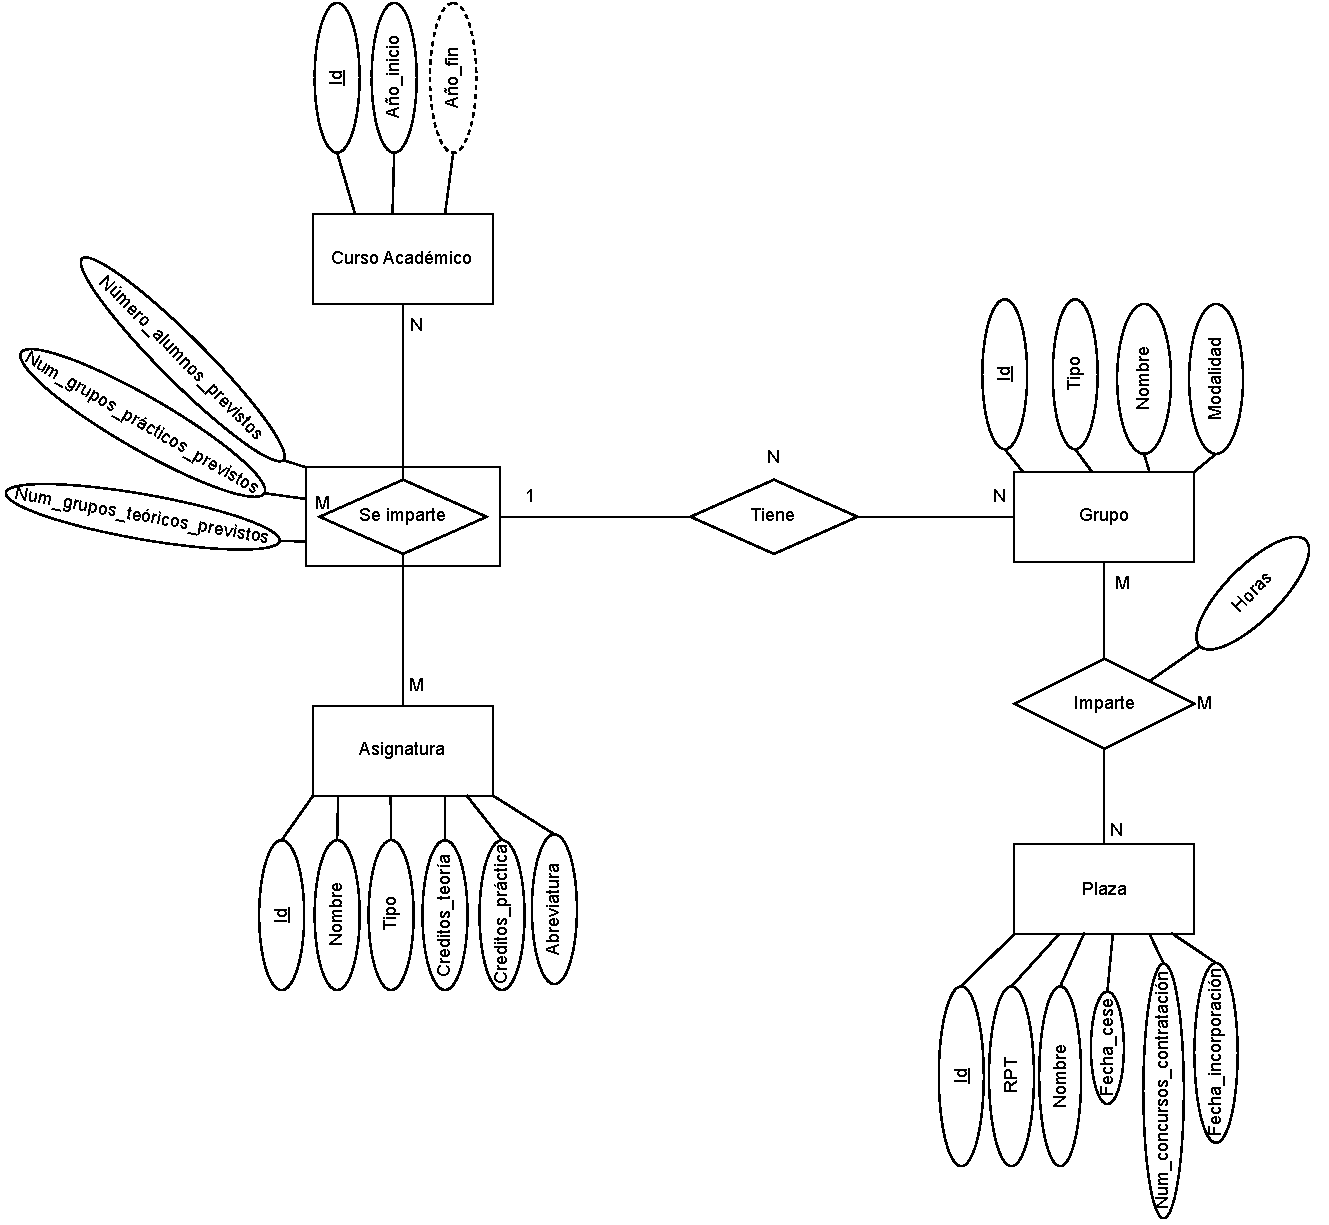
\includegraphics[scale=0.8]{../img/Anexos/Casos uso/Vistas ER/Diagrama E-R CU 3.pdf}
	\caption{Vista diagrama entidad relación para el CU-3}\label{er_cu3}
\end{figure}
\FloatBarrier

\newpage
\subsection{Prototipos de vistas de los casos de uso}
\begin{itemize}
	\item \textbf{CU-1.} Mantenimiento académico.
	\begin{itemize}
		\item \textbf{CU-1.1} Mantenimiento de centros.
		\begin{figure}[!h]
		\centering
		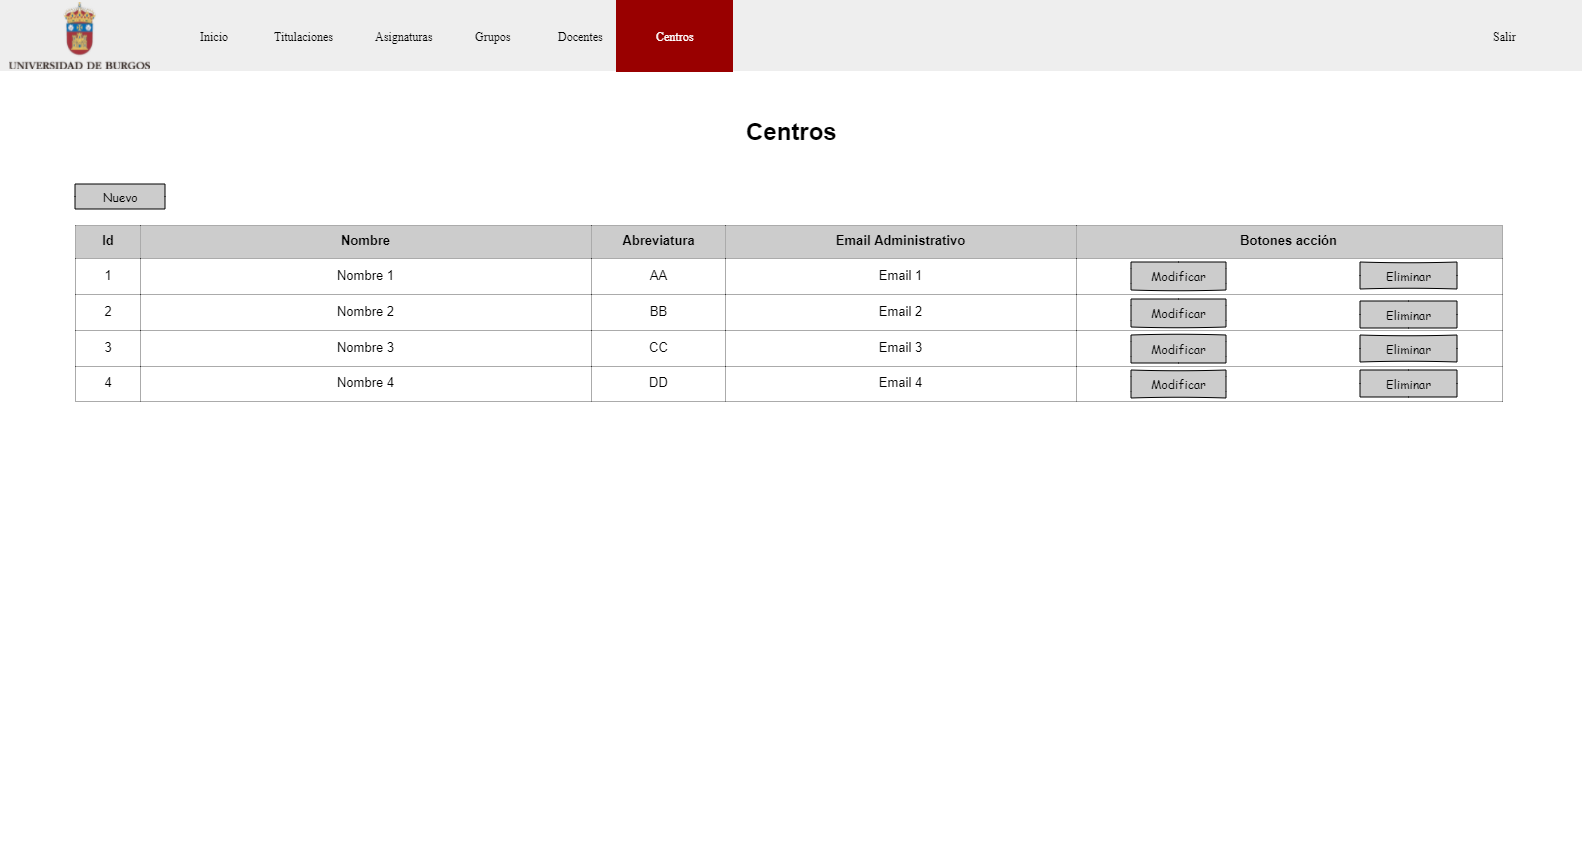
\includegraphics[width=\textwidth]{../img/Anexos/Vistas/centros.png}
		\caption{Mantenimiento de centros}
		\end{figure}
		\FloatBarrier
		\item \textbf{CU-1.1.1} Añadir/Modificar centros.
		\begin{figure}[!h]
		\centering
		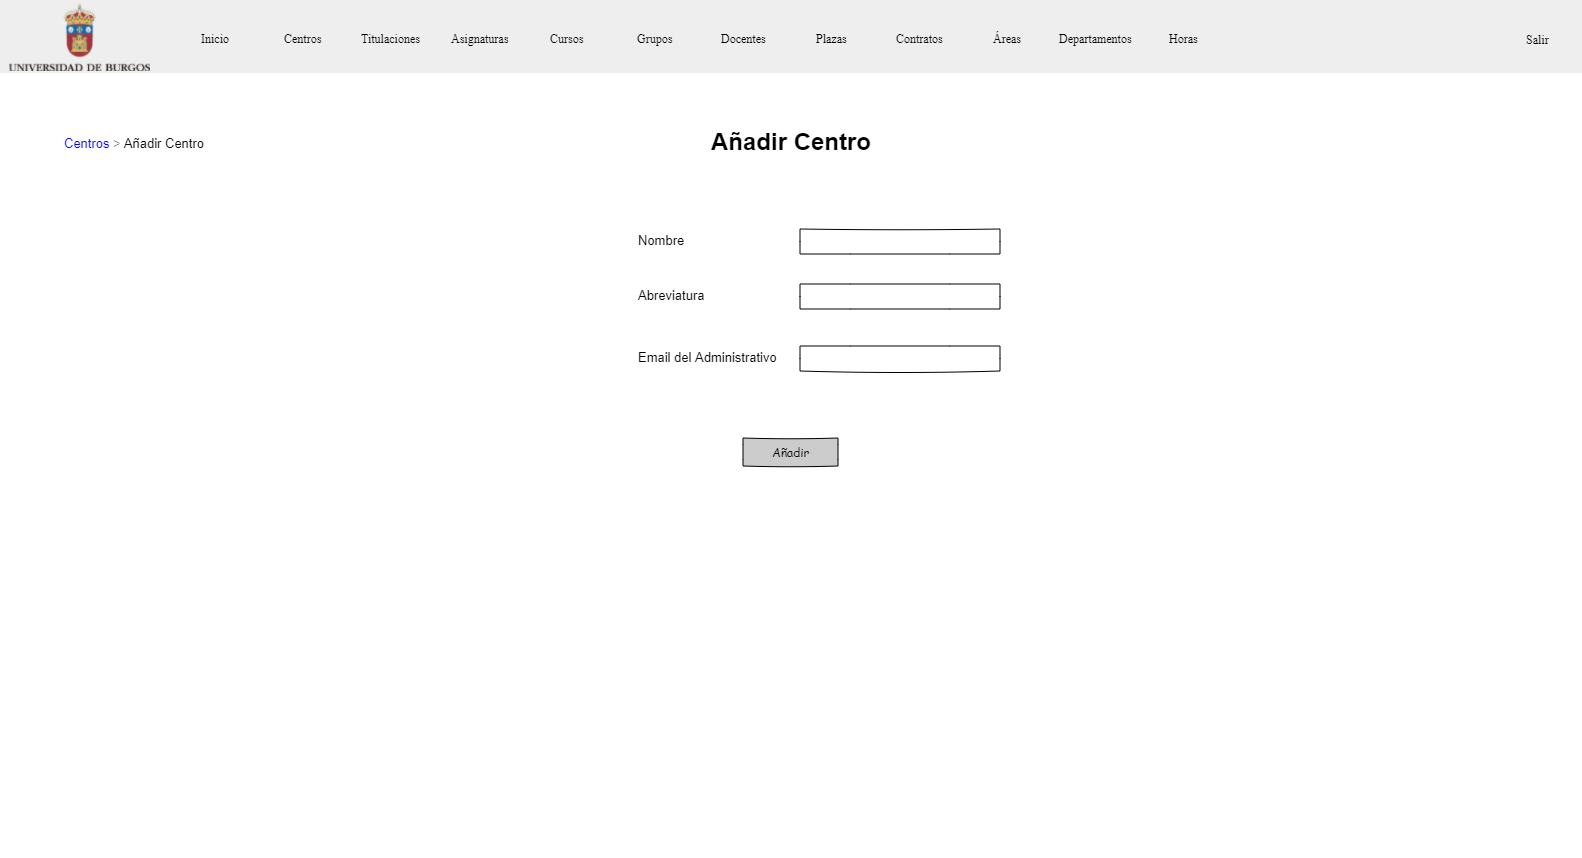
\includegraphics[width=\textwidth]{../img/Anexos/Vistas/add_centro.png}
		\caption{Añadir/Modificar centros}
		\end{figure}
		\FloatBarrier
\newpage
		\item \textbf{CU-1.2} Mantenimiento de titulaciones.
		\begin{figure}[!h]
		\centering
		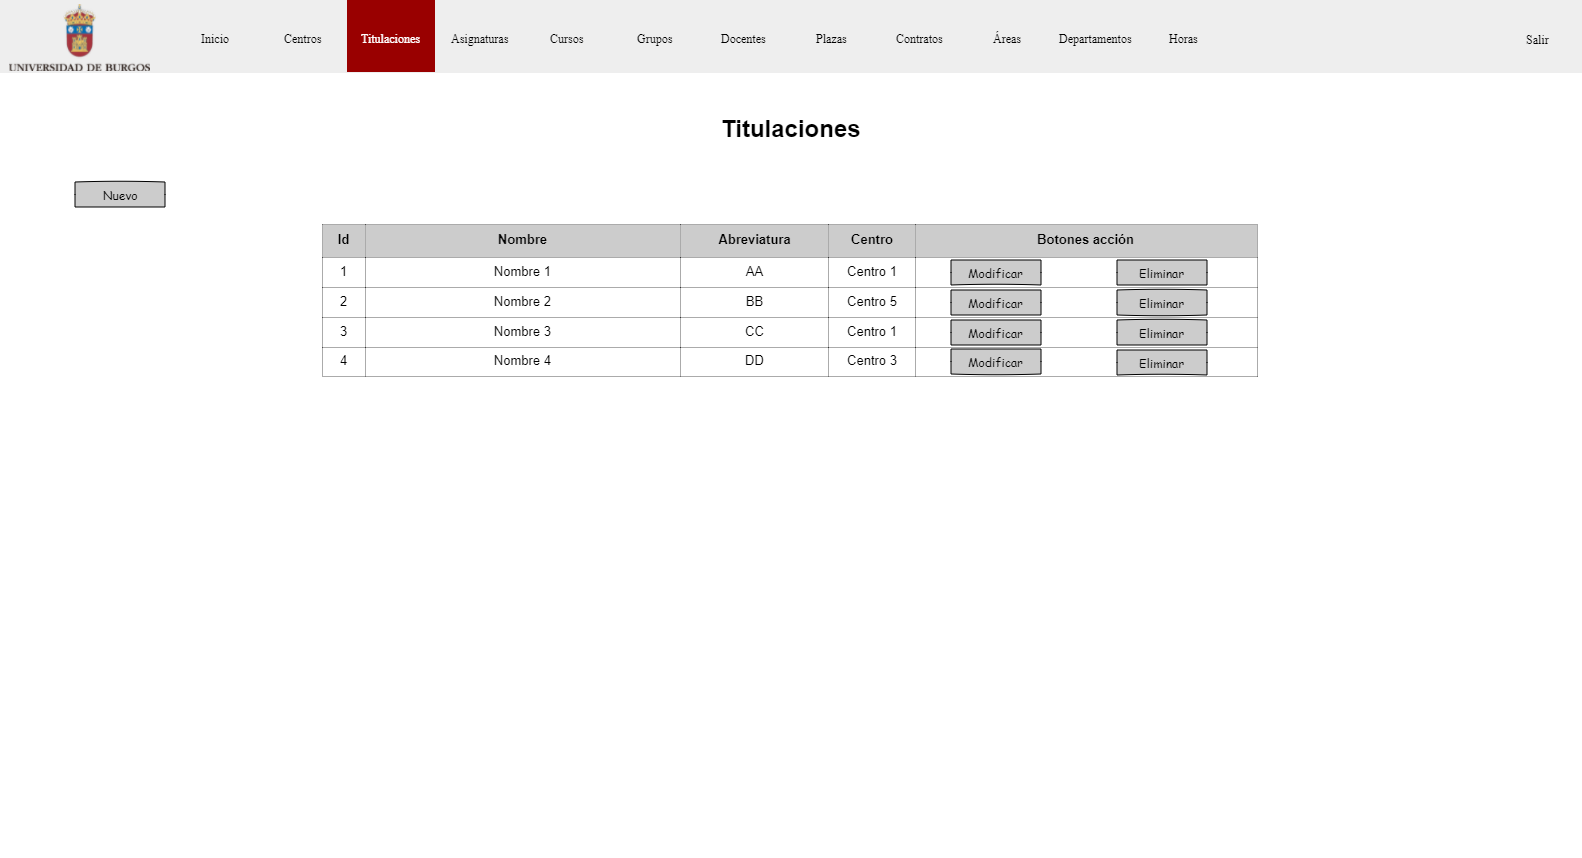
\includegraphics[width=\textwidth]{../img/Anexos/Vistas/titulaciones.png}
		\caption{Mantenimiento de titulaciones}
		\end{figure}
		\FloatBarrier
		\item \textbf{CU-1.2.1} Añadir/Modificar titulaciones.
		\begin{figure}[!h]
		\centering
		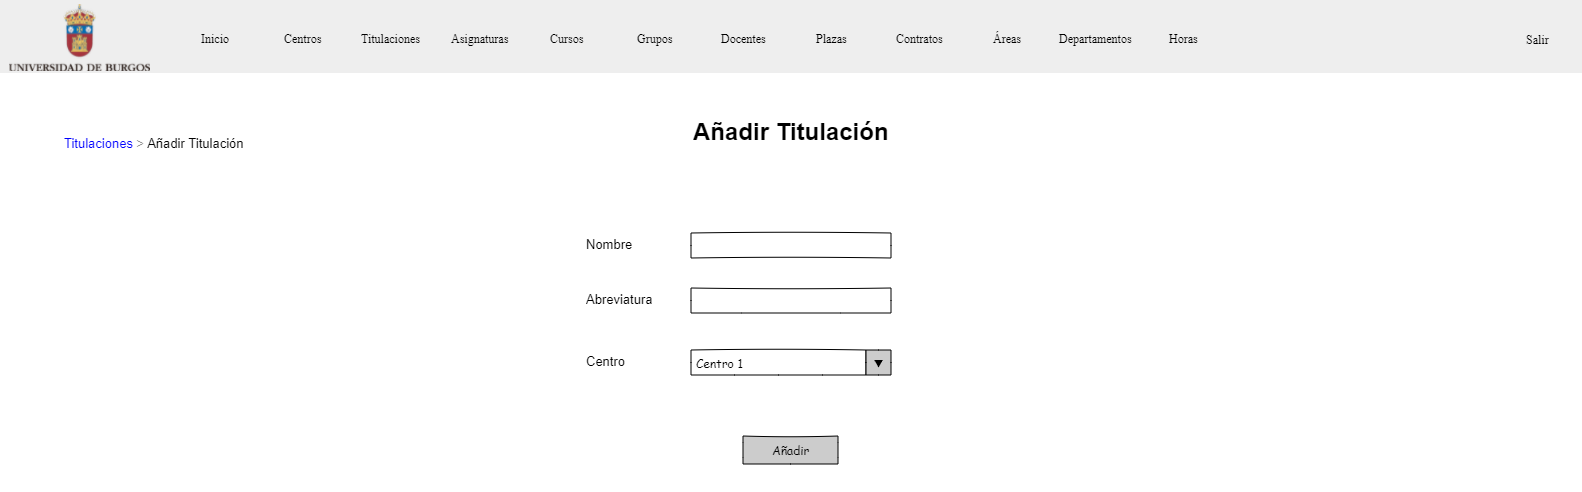
\includegraphics[width=\textwidth]{../img/Anexos/Vistas/add_titulacion.png}
		\caption{Añadir/Modificar titulaciones}
		\end{figure}
		\FloatBarrier
\newpage
		\item \textbf{CU-1.3} Mantenimiento de asignaturas.
		\begin{figure}[!h]
		\centering
		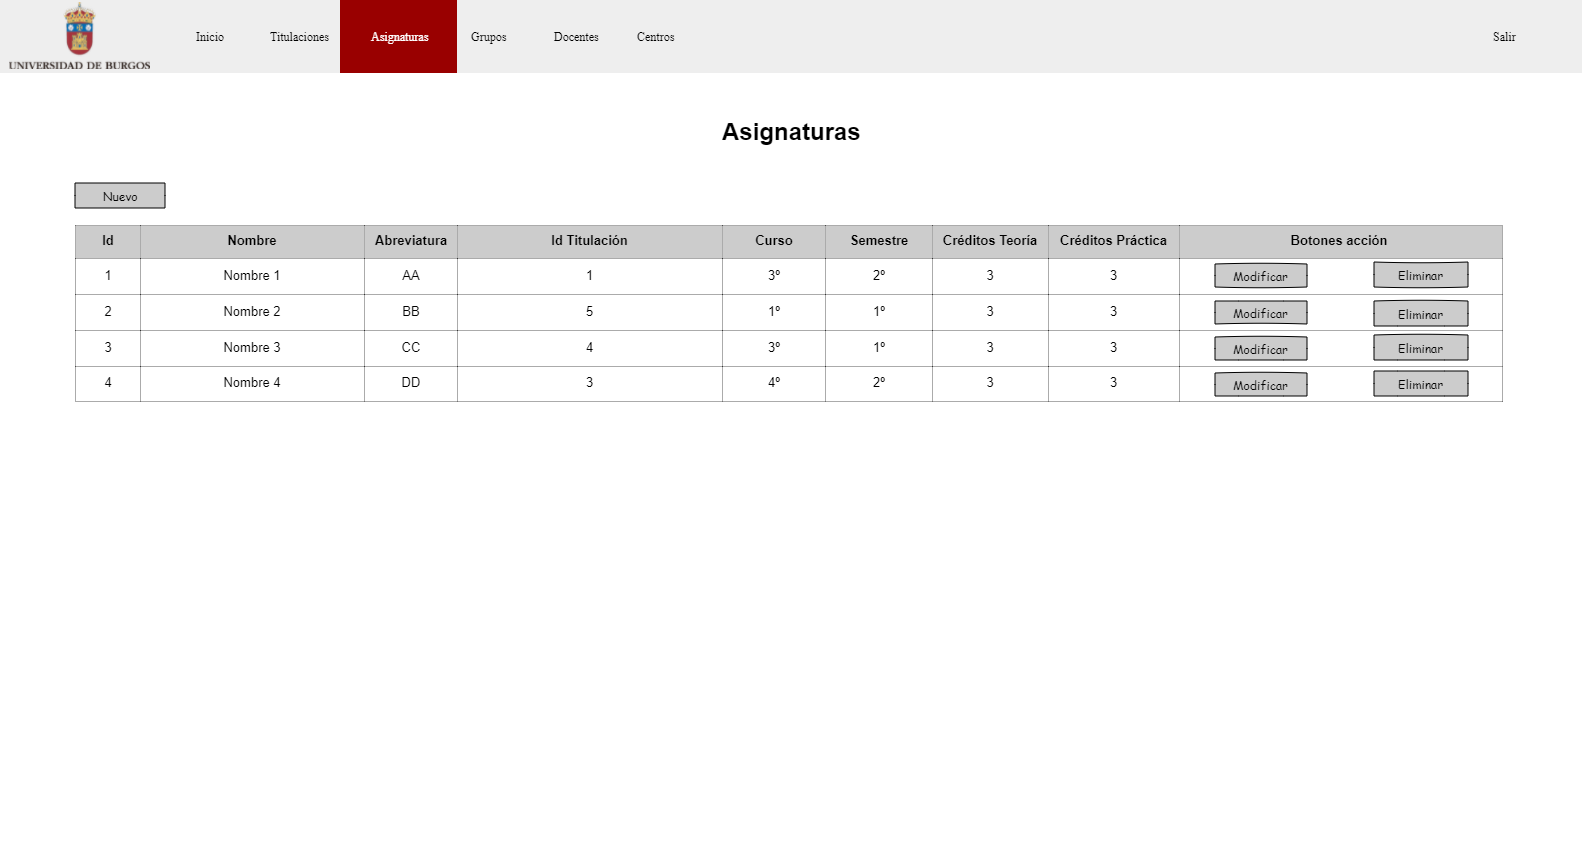
\includegraphics[width=\textwidth]{../img/Anexos/Vistas/asignaturas.png}
		\caption{Mantenimiento de asignaturas}
		\end{figure}
		\FloatBarrier
		\item \textbf{CU-1.3.1} Añadir/Modificar asignaturas.
		\begin{figure}[!h]
		\centering
		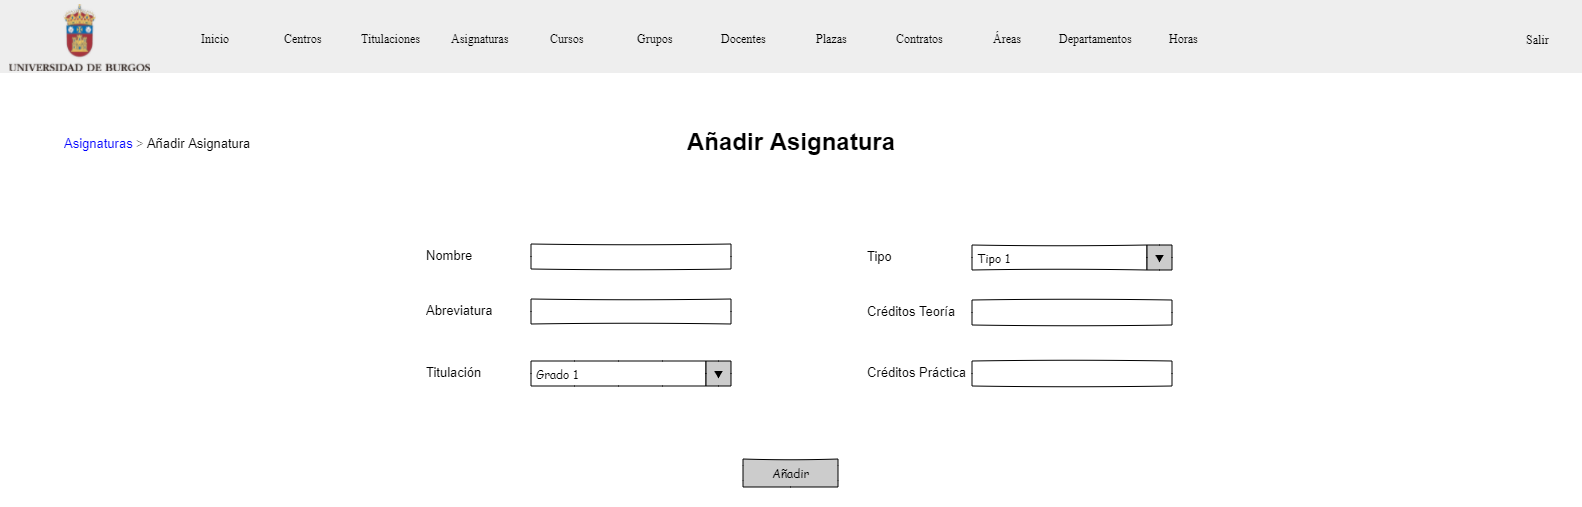
\includegraphics[width=\textwidth]{../img/Anexos/Vistas/add_asignatura.png}
		\caption{Añadir/Modificar asignaturas}
		\end{figure}
		\FloatBarrier
	\end{itemize}
	
\newpage	
	\item \textbf{CU-2.} Mantenimiento de profesorado.
	\begin{itemize}
		\item \textbf{CU-2.1} Mantenimiento de departamentos.
		\begin{figure}[!h]
		\centering
		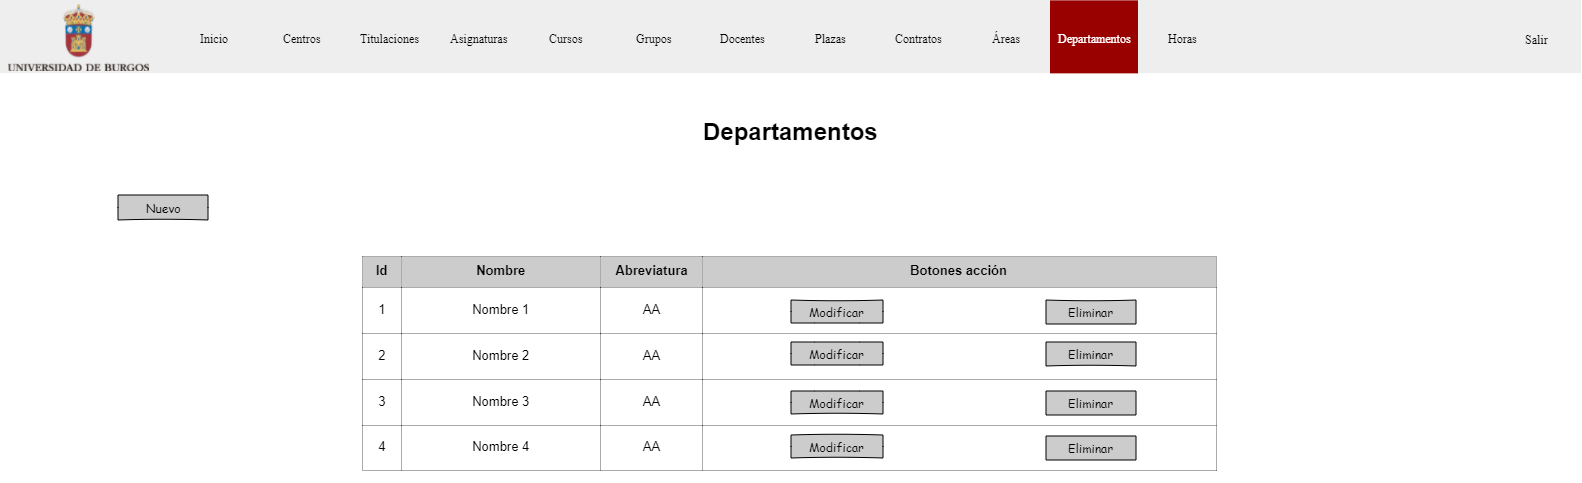
\includegraphics[width=\textwidth]{../img/Anexos/Vistas/departamentos.png}
		\caption{Mantenimiento de departamentos}
		\end{figure}
		\FloatBarrier
		\item \textbf{CU-2.1.1} Añadir/Modificar departamentos.
		\begin{figure}[!h]
		\centering
		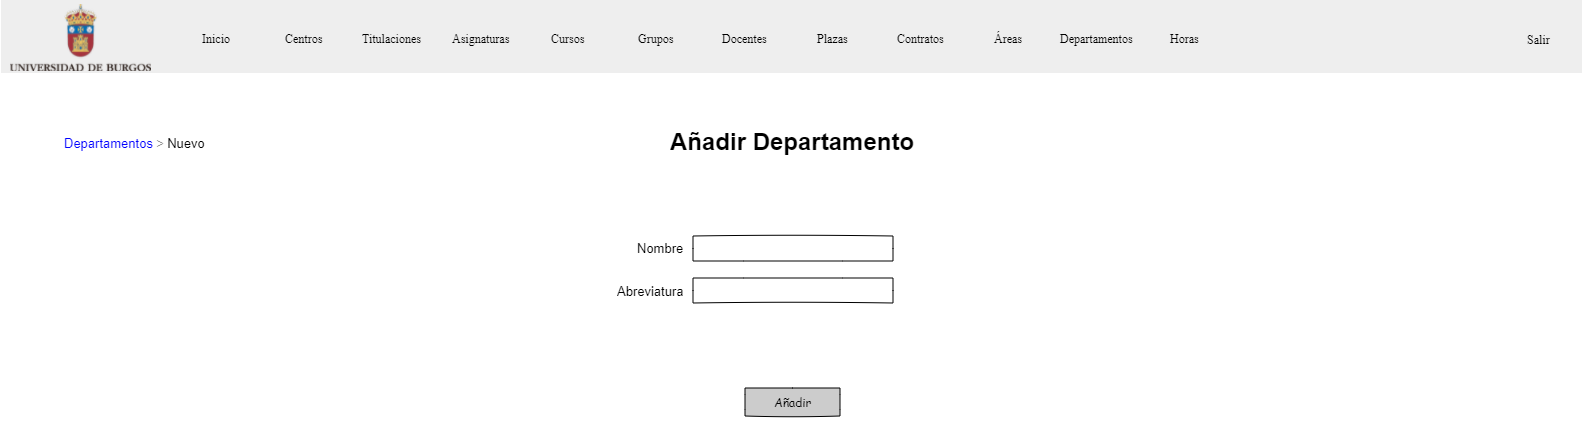
\includegraphics[width=\textwidth]{../img/Anexos/Vistas/add_departamento.png}
		\caption{Añadir/Modificar departamentos}
		\end{figure}
		\FloatBarrier
\newpage
		\item \textbf{CU-2.2} Mantenimiento de áreas.
		\begin{figure}[!h]
		\centering
		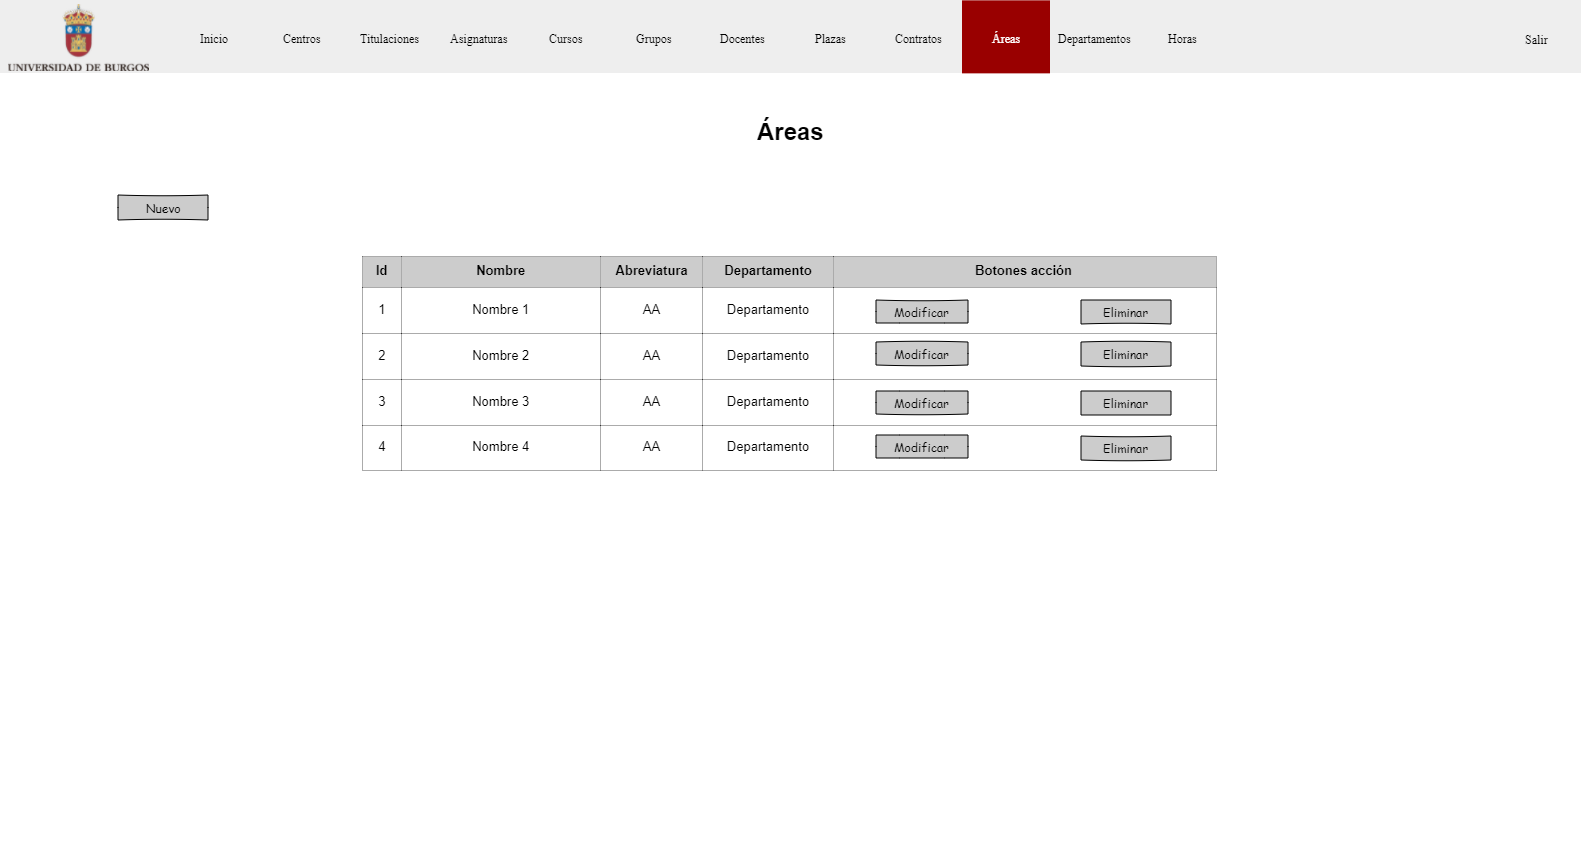
\includegraphics[width=\textwidth]{../img/Anexos/Vistas/areas.png}
		\caption{Mantenimiento de áreas}
		\end{figure}
		\FloatBarrier
		\item \textbf{CU-2.2.1} Añadir/Modificar áreas.
		\begin{figure}[!h]
		\centering
		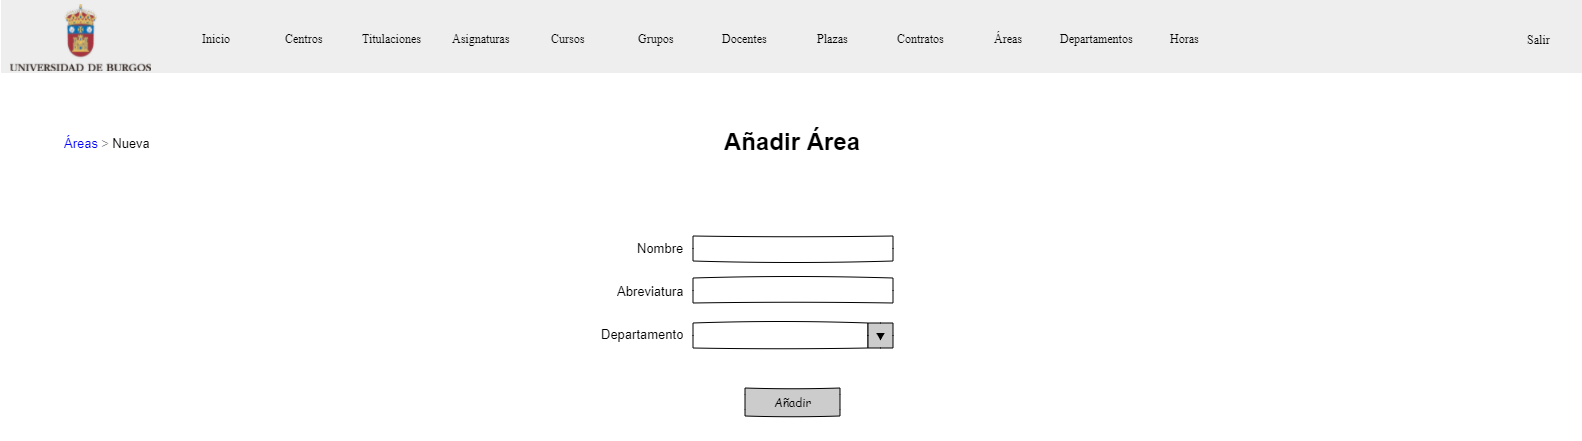
\includegraphics[width=\textwidth]{../img/Anexos/Vistas/add_area.png}
		\caption{Añadir/Modificar áreas}
		\end{figure}
		\FloatBarrier
		\item \textbf{CU-2.3} Mantenimiento de docentes.
		\begin{figure}[!h]
		\centering
		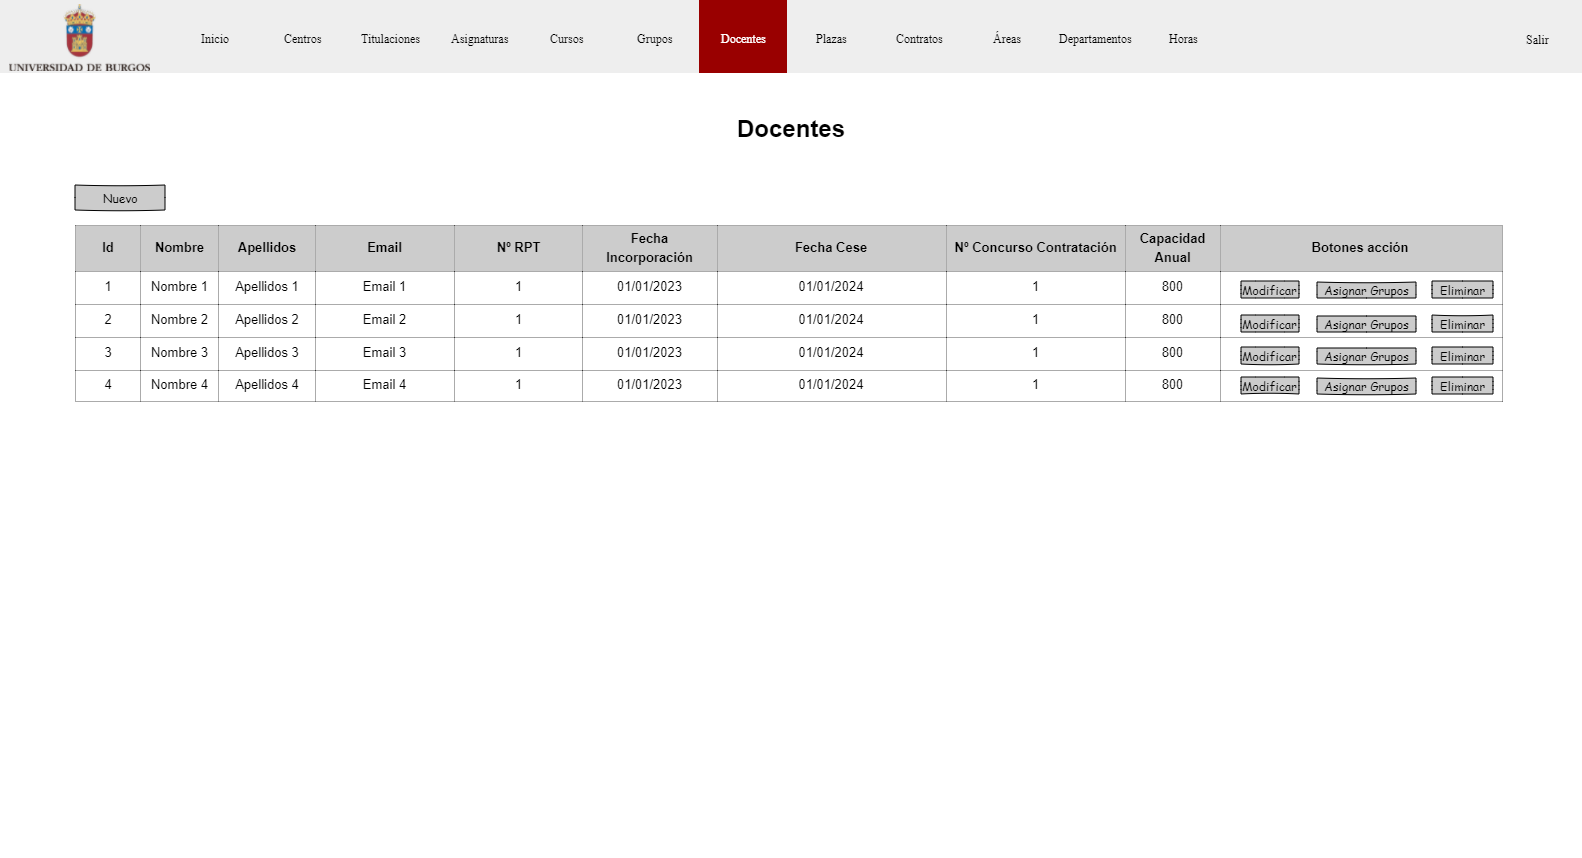
\includegraphics[width=\textwidth]{../img/Anexos/Vistas/docentes.png}
		\caption{Mantenimiento de docentes}
		\end{figure}
		\FloatBarrier
\newpage
		\item \textbf{CU-2.3.1} Añadir/Modificar docentes.
		\begin{figure}[!h]
		\centering
		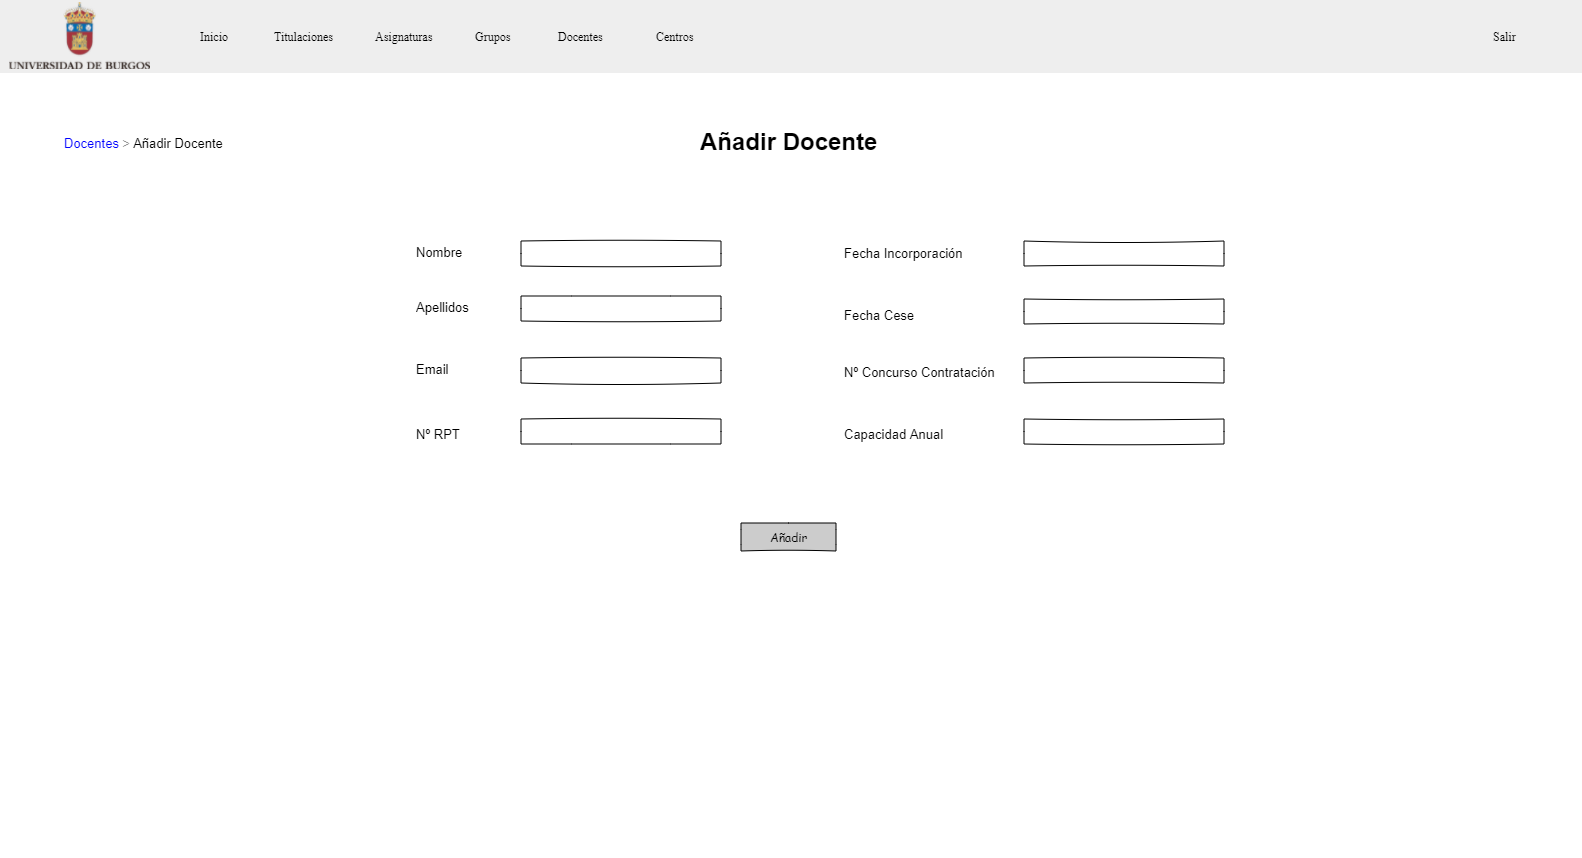
\includegraphics[width=\textwidth]{../img/Anexos/Vistas/add_docente.png}
		\caption{Añadir/Modificar docentes}
		\end{figure}
		\FloatBarrier
		\item \textbf{CU-2.4} Mantenimiento de tipos de contrato.
		\begin{figure}[!h]
		\centering
		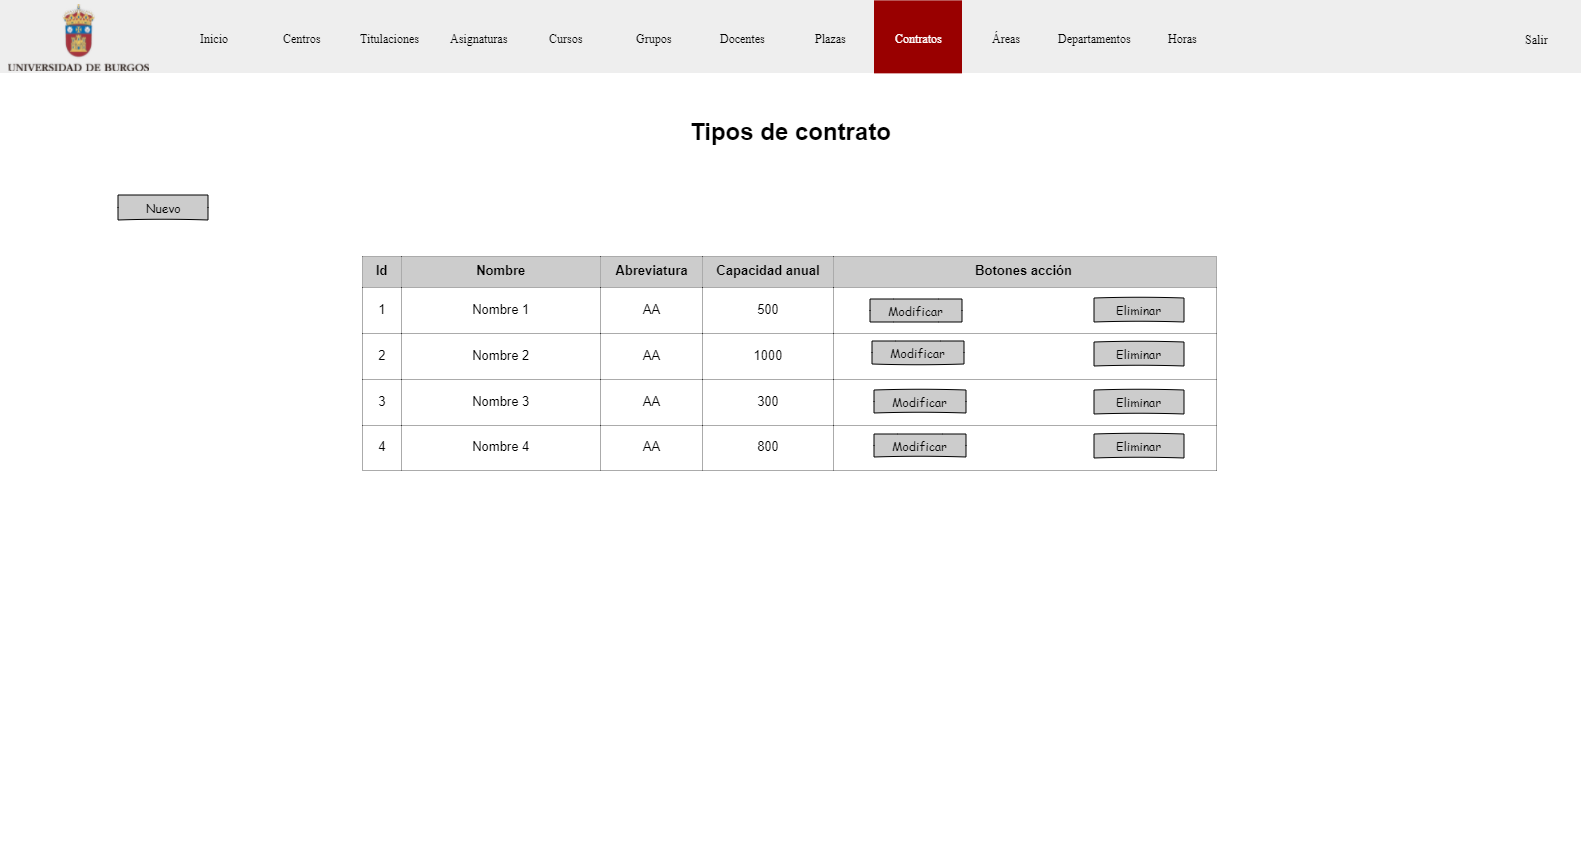
\includegraphics[width=\textwidth]{../img/Anexos/Vistas/contratos.png}
		\caption{Mantenimiento de tipos de contrato}
		\end{figure}
		\FloatBarrier
\newpage
		\item \textbf{CU-2.4.1} Añadir/Modificar tipos de contrato.
		\begin{figure}[!h]
		\centering
		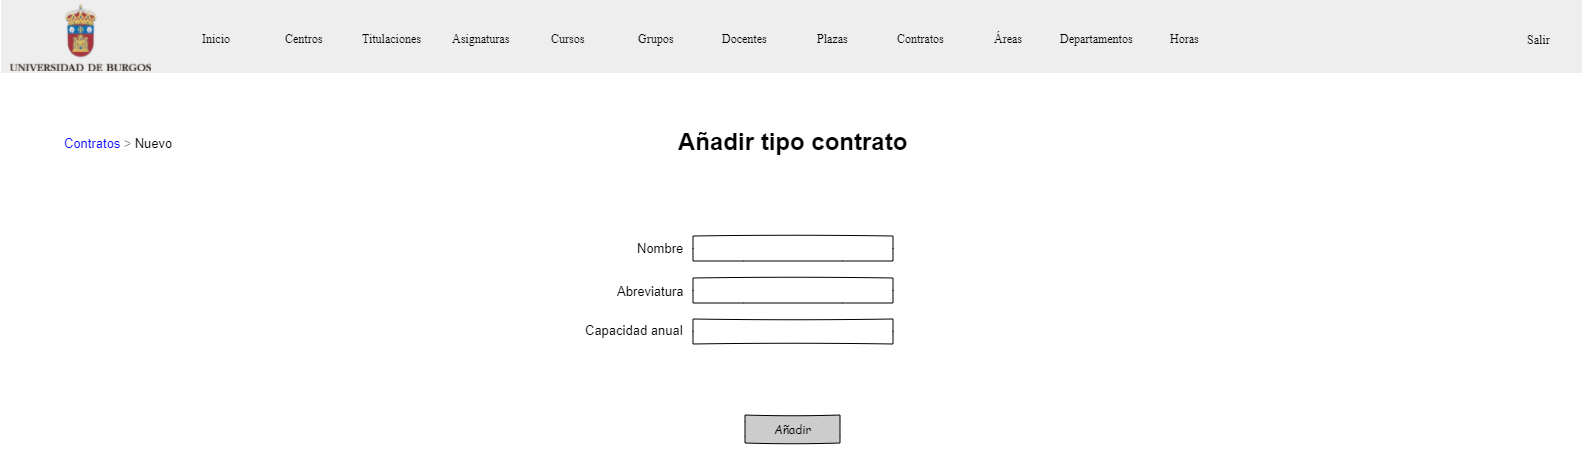
\includegraphics[width=\textwidth]{../img/Anexos/Vistas/add_contrato.png}
		\caption{Añadir/Modificar tipos de contrato}
		\end{figure}
		\FloatBarrier
		\item \textbf{CU-2.5} Mantenimiento de plazas.
		\begin{figure}[!h]
		\centering
		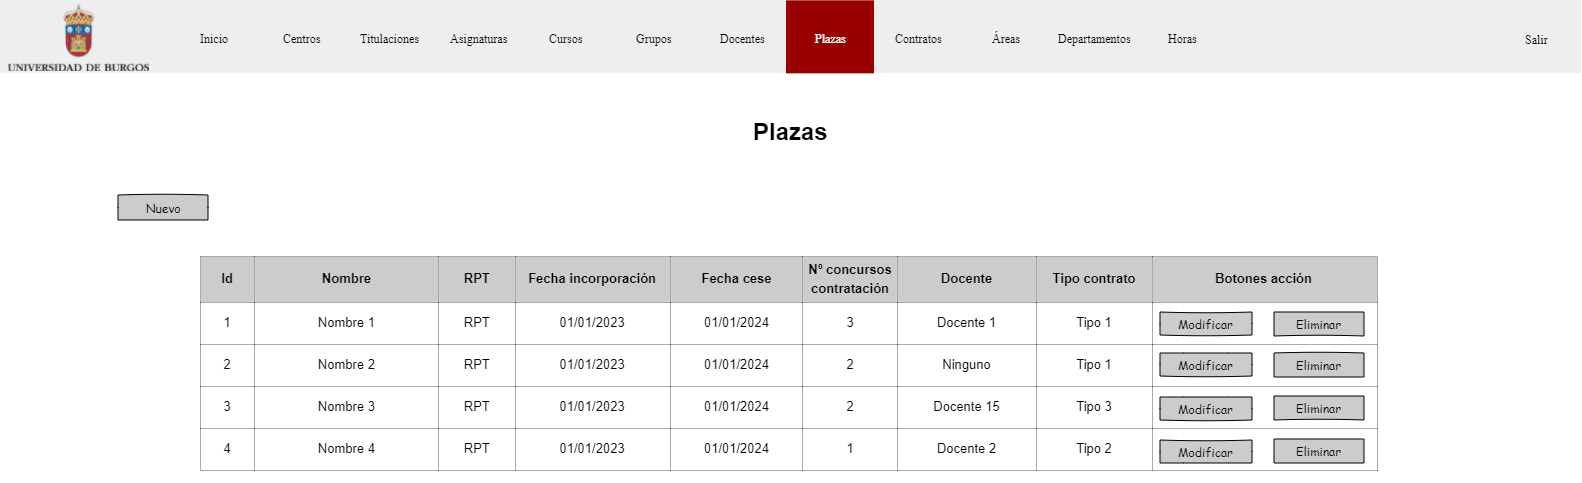
\includegraphics[width=\textwidth]{../img/Anexos/Vistas/plazas.png}
		\caption{Mantenimiento de plazas}
		\end{figure}
		\FloatBarrier
\newpage
		\item \textbf{CU-2.5.1} Añadir/Modificar plazas.
		\begin{figure}[!h]
		\centering
		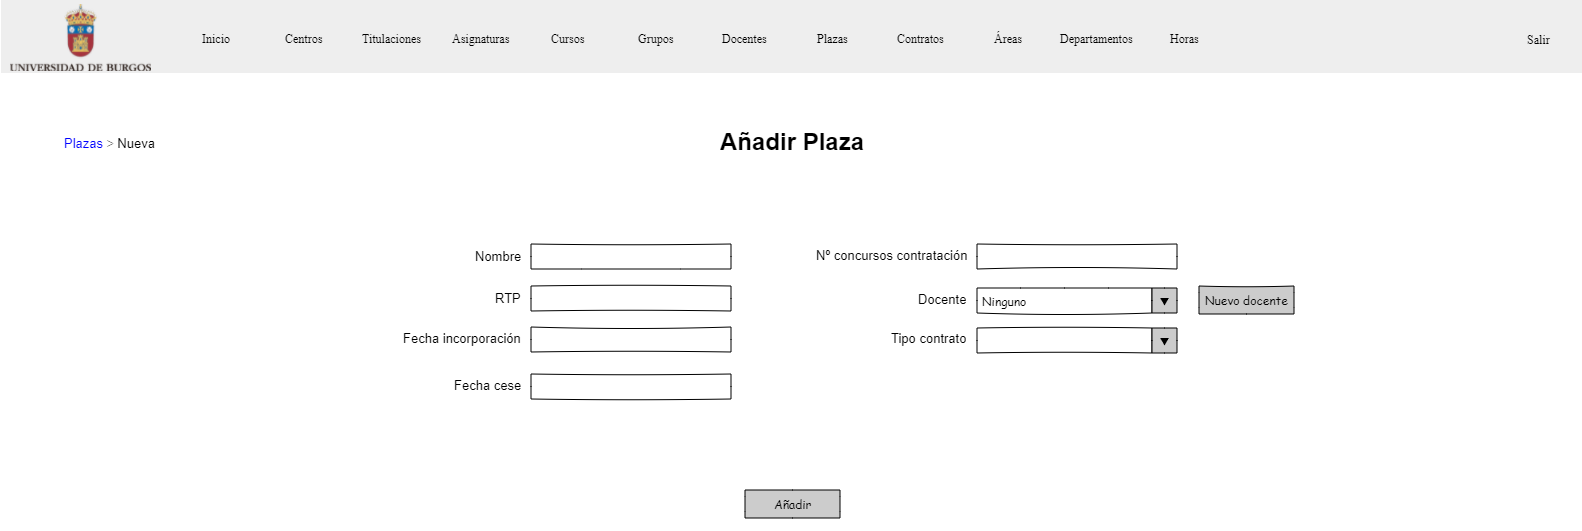
\includegraphics[width=\textwidth]{../img/Anexos/Vistas/add_plaza.png}
		\caption{Añadir/Modificar plazas}
		\end{figure}
		\FloatBarrier
		\item \textbf{CU-2.6} Asignar plaza a docente.
		\begin{figure}[!h]
		\centering
		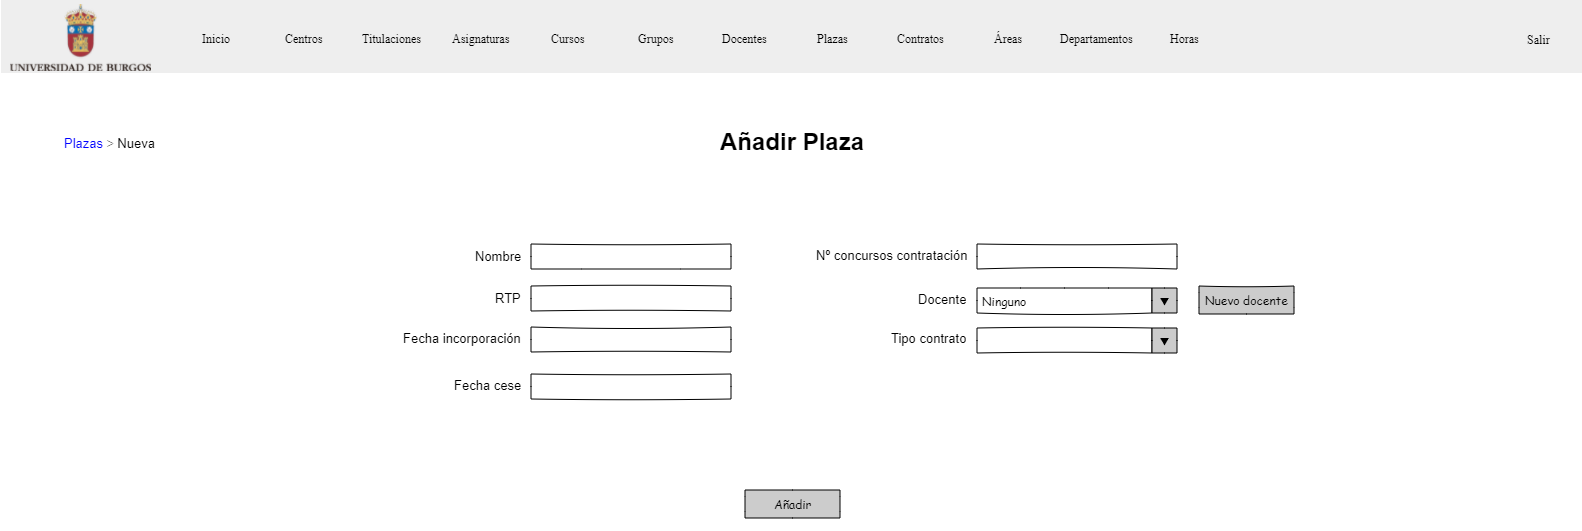
\includegraphics[width=\textwidth]{../img/Anexos/Vistas/add_plaza.png}
		\caption{Asignar plaza a docente}
		\end{figure}
		\FloatBarrier
	\end{itemize}
	
\newpage
	\item \textbf{CU-3.} Asignación docente.
	\begin{itemize}
		\item \textbf{CU-3.1} Mantenimiento cursos académicos.
		\begin{figure}[!h]
		\centering
		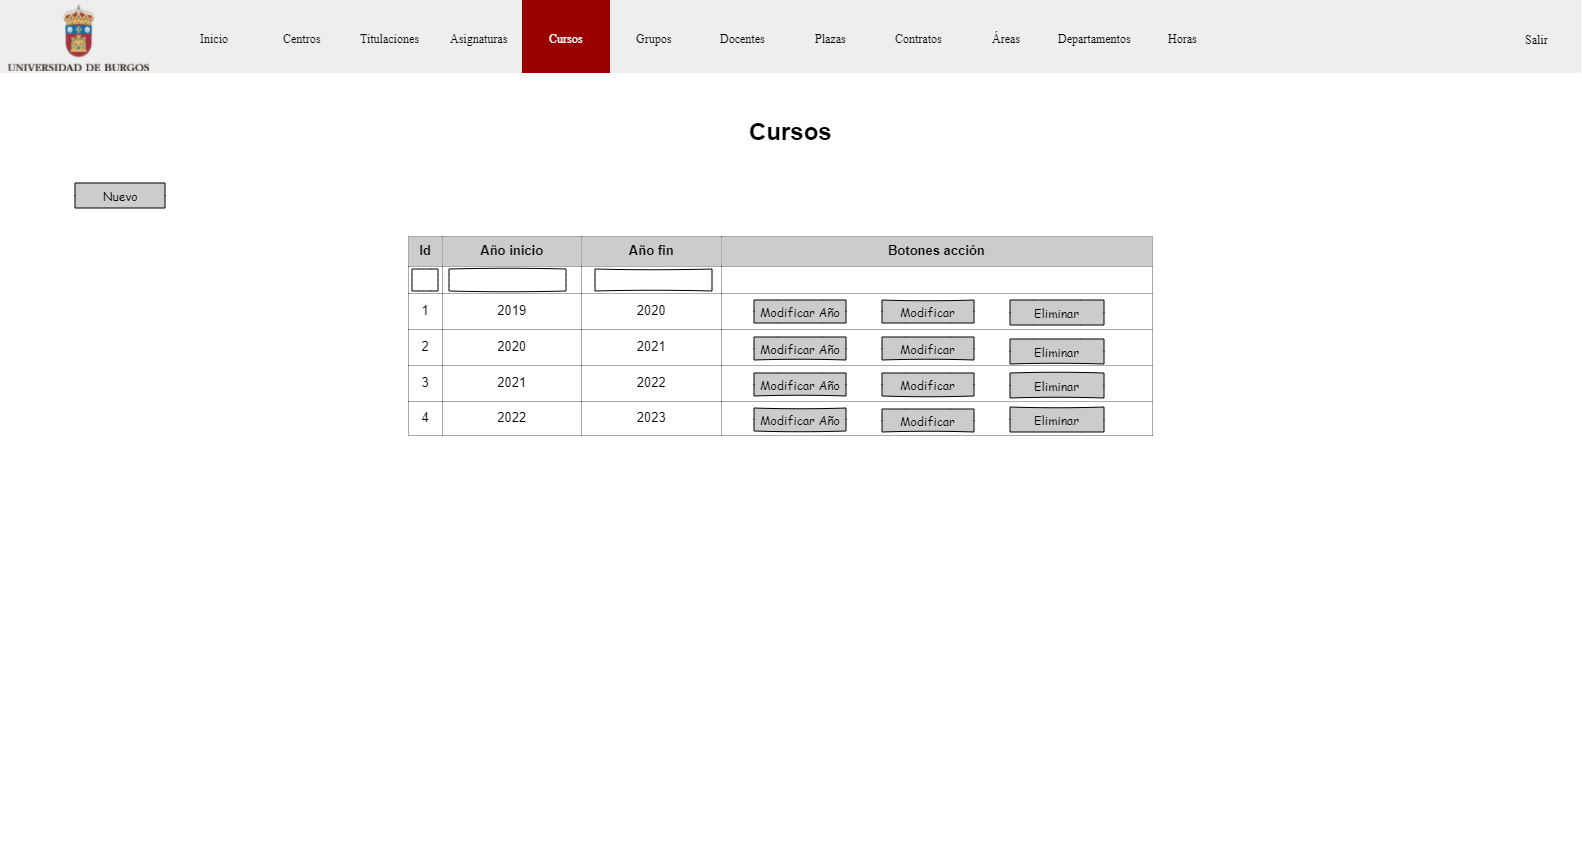
\includegraphics[width=\textwidth]{../img/Anexos/Vistas/cursos.png}
		\caption{Mantenimiento cursos académicos}
		\end{figure}
		\FloatBarrier
		\begin{figure}[!h]
		\centering
		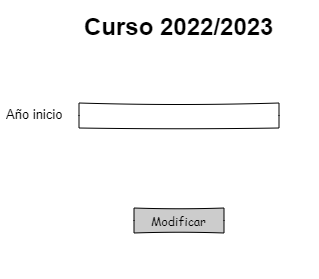
\includegraphics[width=0.5\textwidth]{../img/Anexos/Vistas/mod_ano_curso.png}
		\caption{Modificar año curso académico}
		\end{figure}
		\FloatBarrier
\newpage
		\item \textbf{CU-3.1.1} Añadir curso académico.
		\begin{figure}[!h]
		\centering
		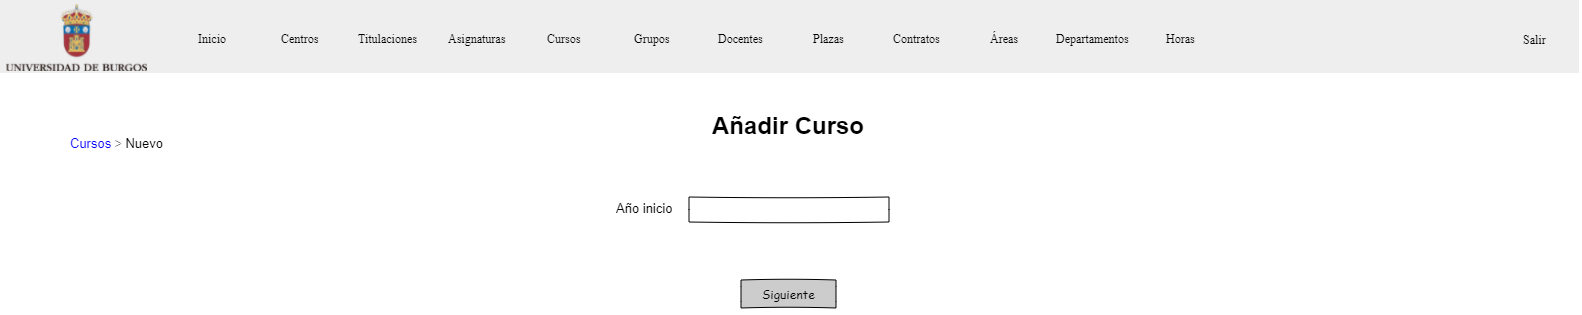
\includegraphics[width=\textwidth]{../img/Anexos/Vistas/add_curso.png}
		\caption{Añadir curso académico}
		\end{figure}
		\FloatBarrier
		\begin{figure}[!h]
		\centering
		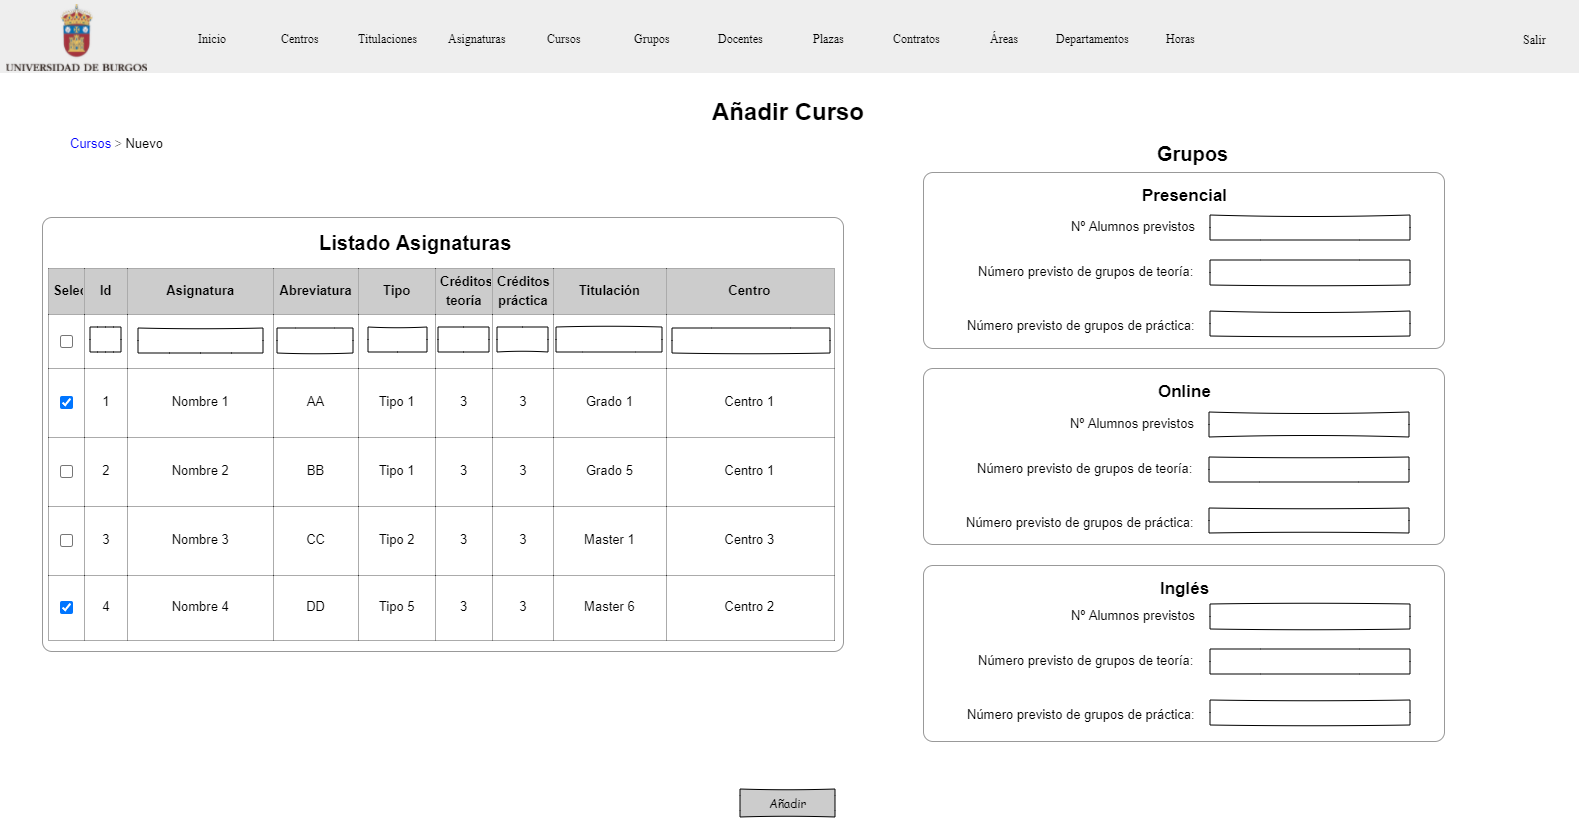
\includegraphics[width=\textwidth]{../img/Anexos/Vistas/add_curso_1.png}
		\caption{Añadir curso académico 2}
		\end{figure}
		\FloatBarrier
\newpage
		\item \textbf{CU-3.1.2} Modificar curso académico.
		\begin{figure}[!h]
		\centering
		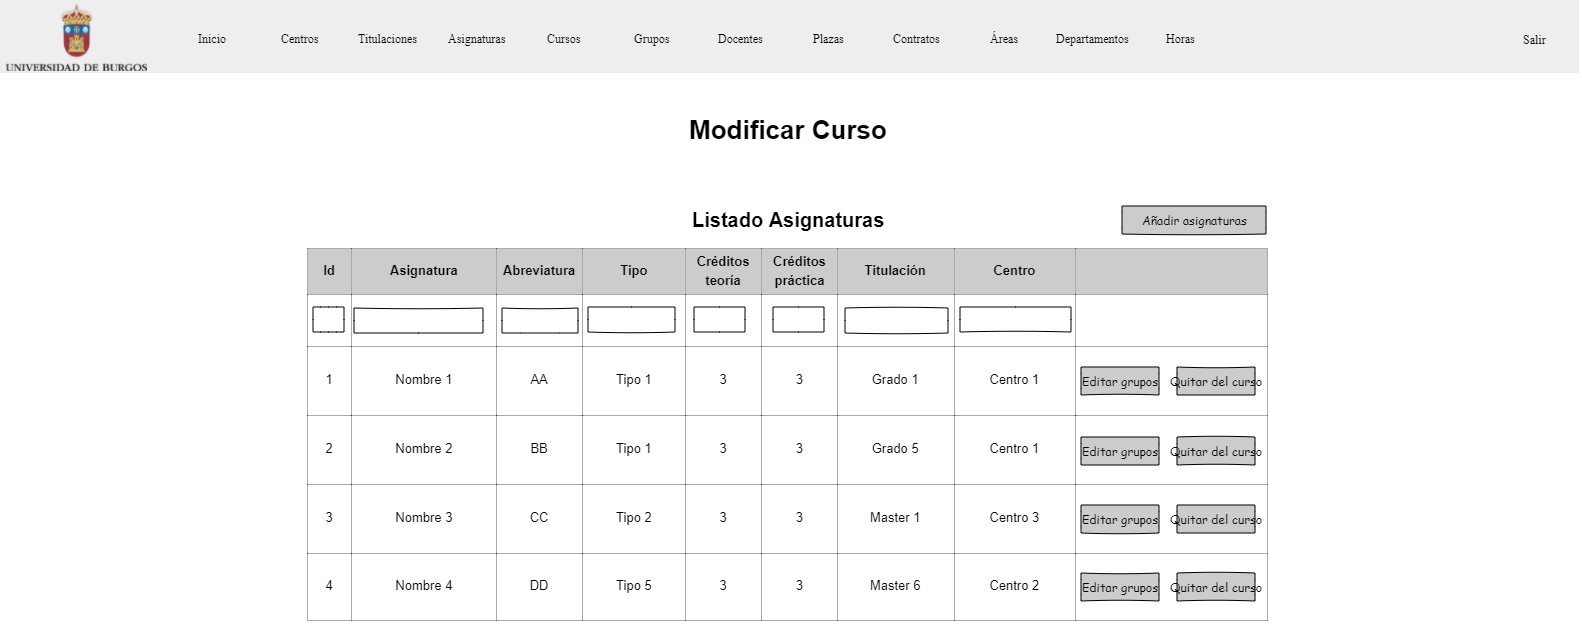
\includegraphics[width=\textwidth]{../img/Anexos/Vistas/mod_curso.png}
		\caption{Modificar curso académico}
		\end{figure}
		\FloatBarrier
		\begin{figure}[!h]
		\centering
		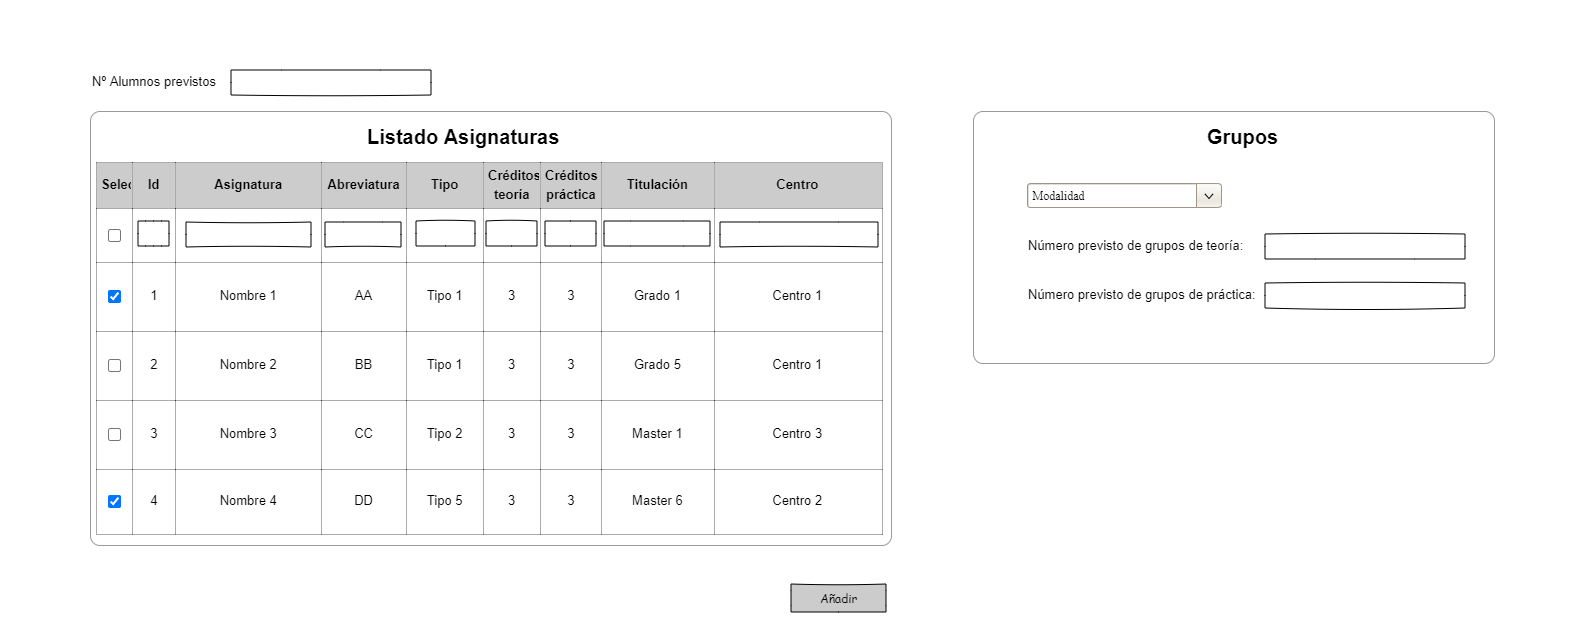
\includegraphics[width=\textwidth]{../img/Anexos/Vistas/add_asig.png}
		\caption{Añadir asignaturas al curso}
		\end{figure}
		\FloatBarrier
\newpage
		\item \textbf{CU-3.2} Mantenimiento de grupos.
		\begin{figure}[!h]
		\centering
		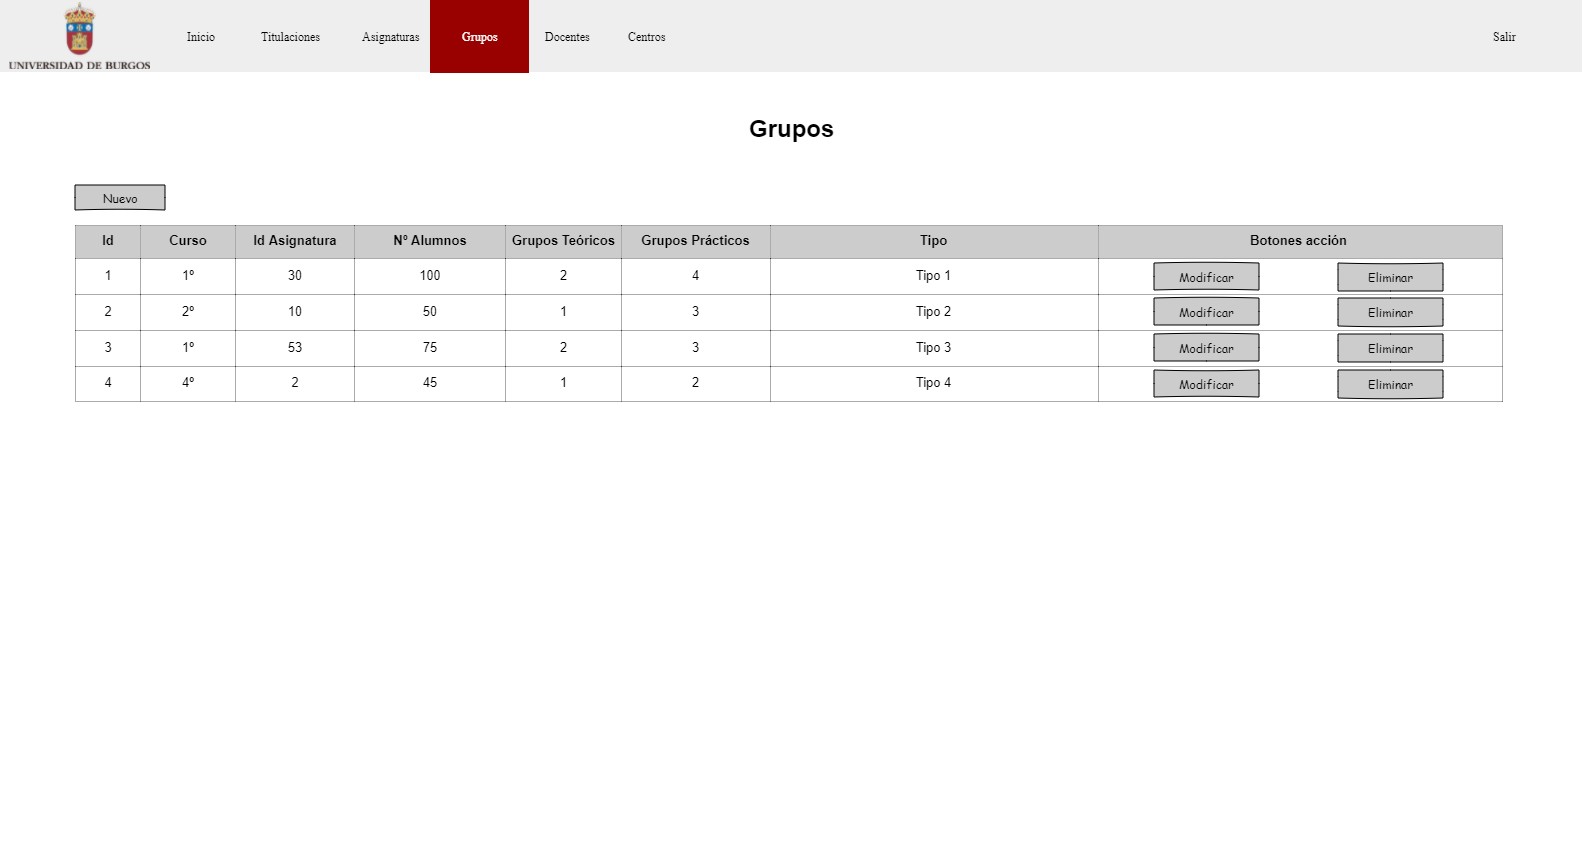
\includegraphics[width=\textwidth]{../img/Anexos/Vistas/grupos.png}
		\caption{Mantenimiento de grupos}
		\end{figure}
		\FloatBarrier
		\item \textbf{CU-3.2.1} Añadir/Modificar grupo.
		\begin{figure}[!h]
		\centering
		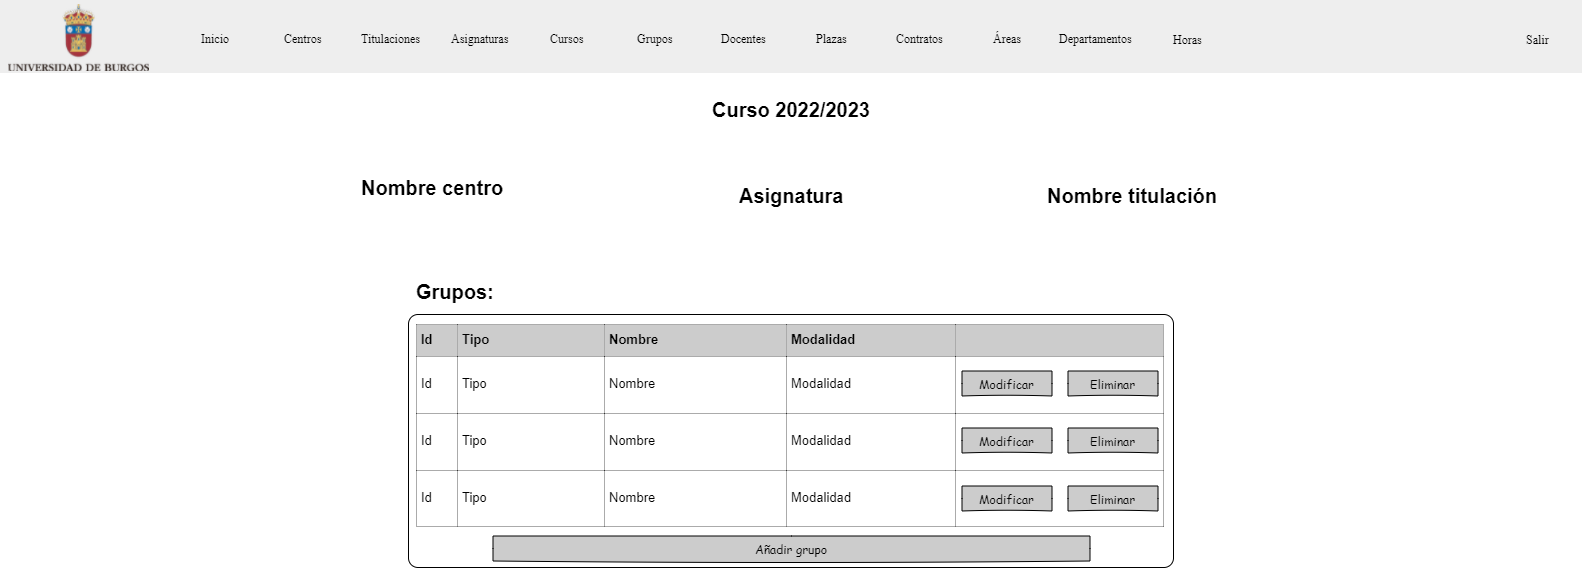
\includegraphics[width=\textwidth]{../img/Anexos/Vistas/addmod_grupo.png}
		\caption{Añadir/Modificar grupo}
		\end{figure}
		\FloatBarrier
		\begin{figure}[!h]
		\centering
		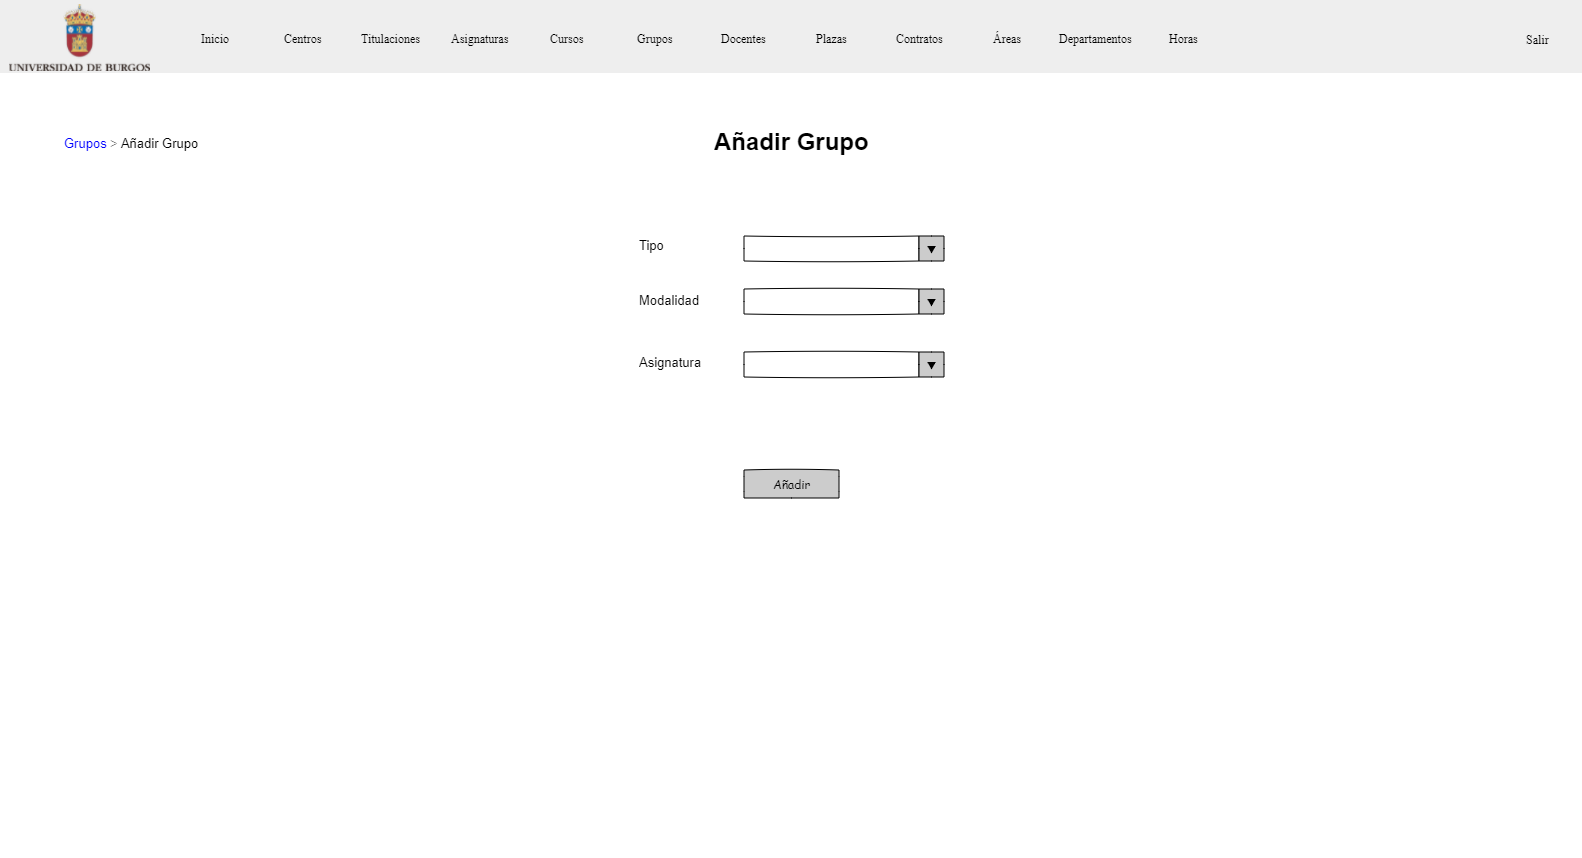
\includegraphics[width=0.5\textwidth]{../img/Anexos/Vistas/add_grupo.png}
		\caption{Añadir/Modificar grupo 2}
		\end{figure}
		\FloatBarrier
		\newpage
		\item \textbf{CU-3.3} Asignación de horas de plazas a grupos.
		\begin{figure}[!h]
		\centering
		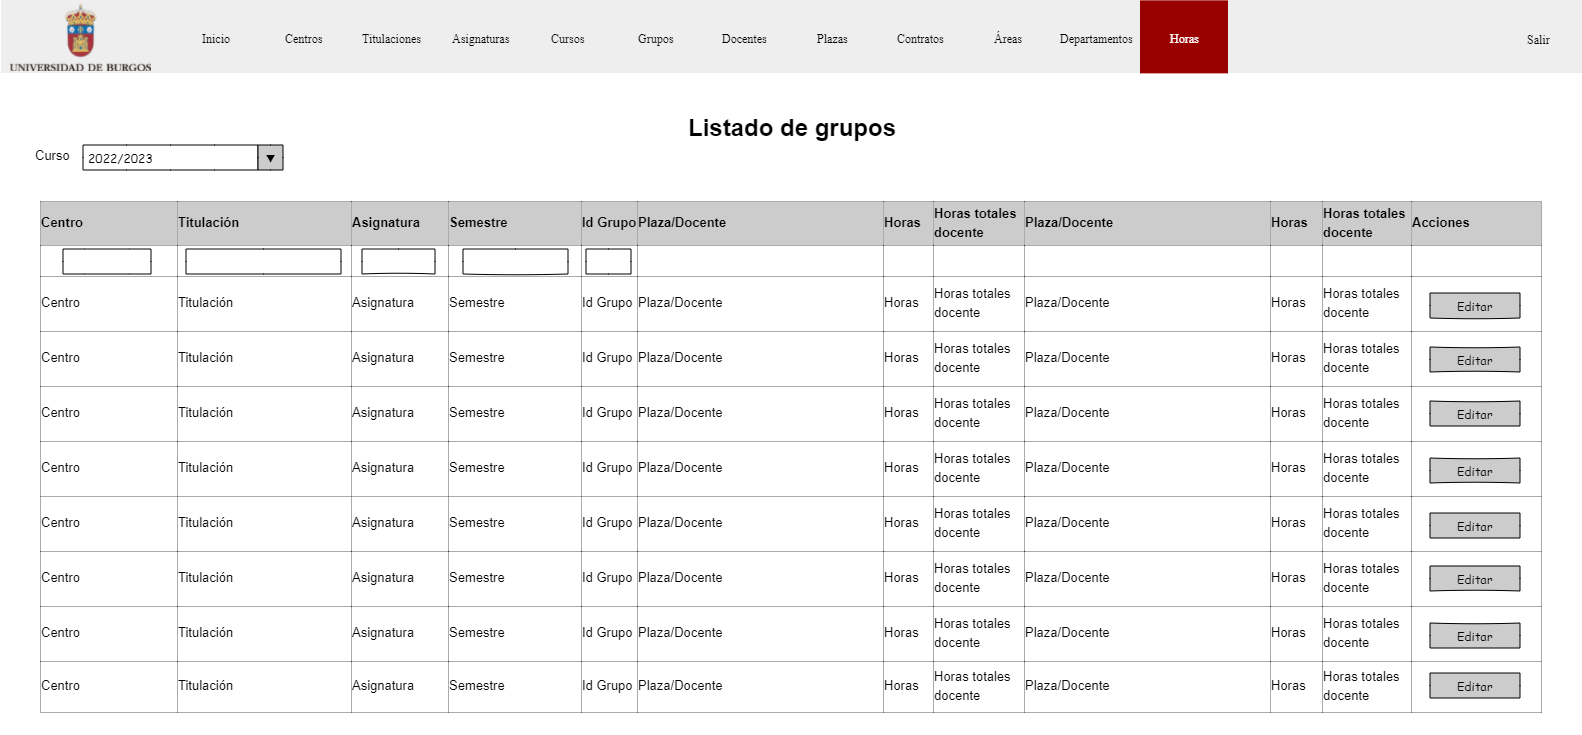
\includegraphics[width=\textwidth]{../img/Anexos/Vistas/horas.png}
		\caption{Asignación de horas de plazas a grupos}
		\end{figure}
		\FloatBarrier
		\begin{figure}[!h]
		\centering
		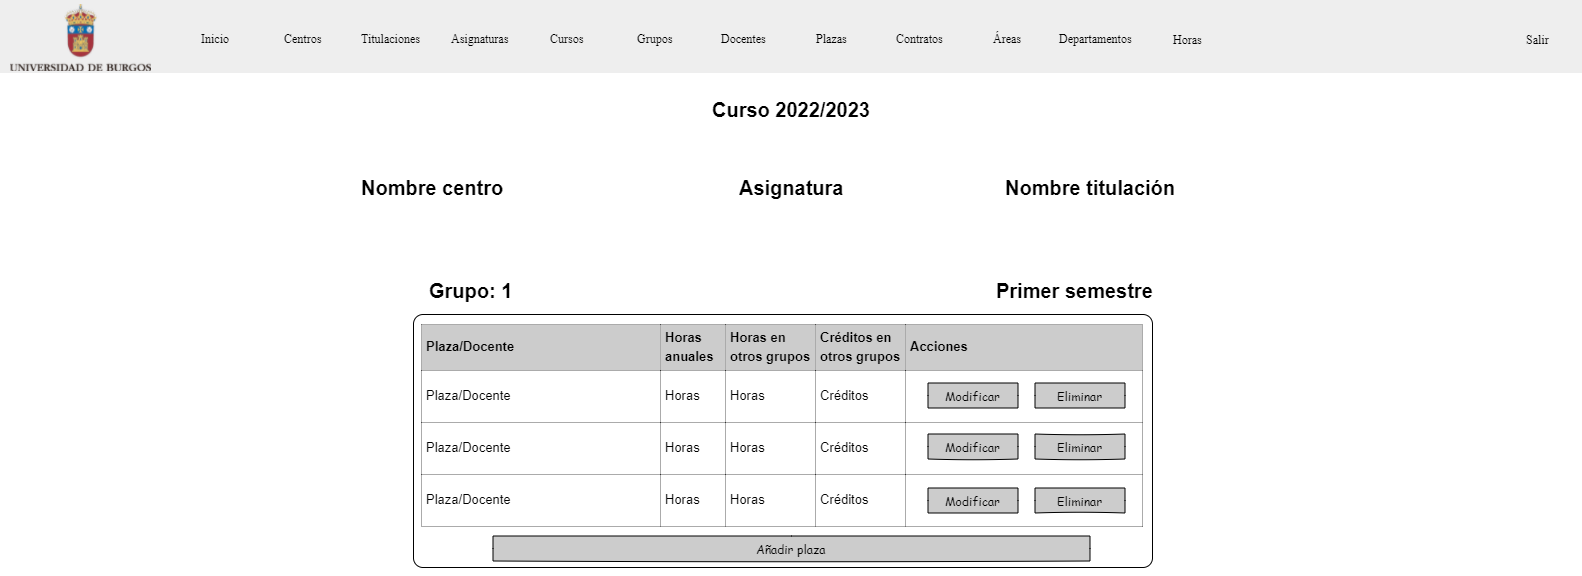
\includegraphics[width=\textwidth]{../img/Anexos/Vistas/asig_horas_plaza_grupo.png}
		\caption{Asignación de horas de plazas a grupos 2}
		\end{figure}
		\FloatBarrier
		\begin{figure}[!h]
		\centering
		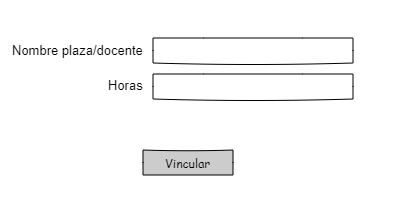
\includegraphics[width=0.5\textwidth]{../img/Anexos/Vistas/asig_horas_plaza_grupo_modal.png}
		\caption{Asignación de horas de plazas a grupos 3}
		\end{figure}
		\FloatBarrier
	\end{itemize}
\end{itemize}



\apendice{Especificación de diseño}

\section{Introducción}
Una vez realizado el estudio y especificación de los requisitos de la aplicación web, se debe realizar el diseño de la misma. En este anexo se pretende aportar información sobre el diseño de los datos que utiliza la aplicación junto al diseño procedimental y arquitectónico del proyecto.

\section{Diseño de datos}
Gracias a la especificación de requisitos y casos de uso, se puede obtener una visión global de la aplicación que permite deducir las entidades, acompañadas de sus datos, necesarias para poder cumplir con lo requerido.

En primer lugar, podemos obtener la visión global de las entidades relacionadas mediante el diagrama general de Entidad-Relación de la figura~\ref{DiagramaGeneralE-R}.

El diagrama obtenido tiene un gran tamaño y, para mejorar la visualización y comprensión del mismo, se ha decidido dividir en vistas donde se incluyan los datos de cada una de las entidades.

La primera vista hace referencia al apartado de mantenimiento académico y se puede ver en la figura~\ref{er_cu1}, la segunda al mantenimiento de profesorado~\ref{er_cu2} y la última a la asignación docente~\ref{er_cu3}.


\figuraApaisadaSinMarco{}{../img/Anexos/Diagrama E-R.pdf}{Diagrama general entidad-relación}{DiagramaGeneralE-R}{}

Del diagrama entidad-relación se puede obtener el diagrama relacional de la figura~\ref{DiagramaRelacional} en el que se pueden ver la tablas que contendrá la base de datos de la aplicación web.

En este diagrama se pueden ver las tablas de la base de datos juntos los distintos campos que tendrá cada una.
Como se puede ver en la figura~\ref{DiagramaRelacional}, las tablas centro, titulación y asignatura tienen un campo llamado código. 
Este código campo podría haber sido utilizado como clave primaria, pero al ser un campo que introduce el usuario, se decidió mantener una clave primaria auto-incremental con la que se hacen las relaciones de las tablas, y además, añadir ese campo para que se puedan hacer búsquedas o filtrar por el mismo sin que su uso pueda afectar a la consistencia del sistema.

Otro aspecto relevante es que en las relaciones que dan lugar a la creación de una tabla intermedia se siguió el mismo patrón que antes. 
Aunque la teoría diga que las claves de las tablas que se relacionan pasan a ser claves primarias de la nueva tabla que se genera, se decidió tener una única clave primaria auto-incremental y tener las claves de las tablas relacionadas como claves foráneas.
De esta manera, las búsquedas en la base de datos estarán más optimizadas al buscar como clave primaria un único campo y no la composición de varios.
Además, se evita cualquier tipo de error de clave primaria al ser la propia base de datos la que asigna esta y no el código creado.

\figuraApaisadaSinMarco{}{../img/Anexos/Diagrama relacional.pdf}{Diagrama relacional}{DiagramaRelacional}{}

\subsection{Diccionario de datos}
A continuación se va a especificar, para cada tabla de la base de datos, el diccionario de datos correspondiente.
De esta forma se pretende facilitar la comprensión de los datos almacenados en la base de datos.

La tabla \texttt{centro} almacena los diferentes centros de la universidad. 
Se puede ver su información en la tabla~\ref{tab:diccionario_centro}.
\begin{table}
\centering
  \begin{tabular}{l p{.2\textwidth} p{.5\textwidth}}
    \toprule
    \textbf{Campo} & \textbf{Tipo} & \textbf{Descripción}\\
    \midrule
    \textbf{\underline{id}} & Entero \underline{PK} & Identificador. Clave primaria creada de forma autoincremental. \\ \addlinespace
    codigo & Entero & Código interno del centro de la universidad. Sólo tiene carácter informativo. \\ \addlinespace 
    abreviatura & Texto & Abreviatura del centro. \\ \addlinespace
    email & Texto & Email administrativo del centro. \\
    \bottomrule
  \end{tabular}
  \caption{Diccionario de datos. Tabla Centro}
  \label{tab:diccionario_centro}
\end{table}

La tabla \texttt{titulación} almacena las titulaciones que son creadas y que pertenecen a un centro.
Se puede ver su información en la tabla~\ref{tab:diccionario_titulacion}.
\begin{table}
  \centering 
  \begin{tabular}{l p{.2\textwidth} p{.5\textwidth}}
    \toprule
    \textbf{Campo} & \textbf{Tipo} & \textbf{Descripción}\\
    \midrule
    \textbf{\underline{id}} & Entero \underline{PK} & Identificador de la titulación. Clave primaria creada de forma autoincremental. \\ \addlinespace
    codigo & Entero & Código interno de la titulación. \\ \addlinespace
    nombre & Texto & Nombre de la titulación. \\ \addlinespace
    abreviatura & Texto & Abreviatura de la titulación. \\ \addlinespace
    url & Texto & Dirección web de la titulación. \\ \addlinespace
    id\_centro & Entero FK(Centro) & Identificador del centro asociado a la titulación. \\
    \bottomrule
  \end{tabular}
  \caption{Diccionario de datos. Tabla Titulación}
  \label{tab:diccionario_titulacion}
\end{table}

La tabla \texttt{asignatura} almacena información sobre las asignaturas, cada asignatura pertenece a una titulación. Se puede ver su información en la tabla~\ref{tab:diccionario_asignatura}.

\begin{table}
  \centering 
  \begin{tabular}{l p{.2\textwidth} p{.5\textwidth}}
    \toprule
    \textbf{Campo} & \textbf{Tipo} & \textbf{Descripción}\\
    \midrule
    \textbf{\underline{id}} & Entero \underline{PK} & Identificador de la asignatura. Clave primaria creada de forma autoincremental. \\ \addlinespace
    codigo & Entero & Código interno de la asignatura. \\ \addlinespace
    nombre & Texto & Nombre de la asignatura. \\ \addlinespace
    tipo & Texto & Tipo de la asignatura. \\ \addlinespace
    creditos\_teoria & Entero & Créditos de teoría de la asignatura. \\ \addlinespace
    creditos\_practica & Entero & Créditos de práctica de la asignatura. \\ \addlinespace
    curso & Texto & Curso al que pertenece la asignatura. \\ \addlinespace
    semestre & Texto & Semestre en el que se imparte la asignatura. \\ \addlinespace
    id\_titulacion & Entero FK(Titulación) & Identificador de la titulación a la que pertenece la asignatura. \\
    \bottomrule
  \end{tabular}
  \caption{Diccionario de datos. Tabla Asignatura}
  \label{tab:diccionario_asignatura}
\end{table}

La tabla \texttt{abreviatura} almacena las abreviaturas de las asignaturas. 
De esta forma se permite que una asignatura pueda tener varias abreviaturas.
Se puede ver su información en la tabla~\ref{tab:diccionario_abreviatura}.

\begin{table}
  \centering 
  \begin{tabular}{l p{.2\textwidth} p{.5\textwidth}}
    \toprule
    \textbf{Campo} & \textbf{Tipo} & \textbf{Descripción}\\
    \midrule
    \textbf{\underline{id}} & Entero \underline{PK} & Identificador de la abreviatura. Clave primaria creada de forma autoincremental. \\ \addlinespace
    abreviatura & Texto & Abreviatura de la asignatura. \\ \addlinespace
    id\_asignatura & Entero FK(Asignatura) & Identificador de la asignatura asociada a la abreviatura. \\
    \bottomrule
  \end{tabular}
  \caption{Diccionario de datos. Tabla Abreviatura}
  \label{tab:diccionario_abreviatura}
\end{table}

La tabla \texttt{curso} almacena información sobre los cursos. Se puede ver su información en la tabla~\ref{tab:diccionario_curso}.

\begin{table}
  \centering 
  \begin{tabular}{l p{.2\textwidth} p{.5\textwidth}}
    \toprule
    \textbf{Campo} & \textbf{Tipo} & \textbf{Descripción}\\
    \midrule
    \textbf{\underline{id}} & Entero \underline{PK} & Identificador del curso. Clave primaria creada de forma autoincremental. \\ \addlinespace
    ano\_inicio & Texto & Año de inicio del curso. \\ \addlinespace
    \bottomrule
  \end{tabular}
  \caption{Diccionario de datos. Tabla Curso}
  \label{tab:diccionario_curso}
\end{table}

La tabla \texttt{curso\_asignatura} almacena la relación entre cursos y asignaturas. 
Se puede ver su información en la tabla~\ref{tab:diccionario_curso_asignatura}.

\begin{table}
  \centering
  \begin{tabular}{l p{.2\textwidth} p{.25\textwidth}}
    \toprule
    \textbf{Campo} & \textbf{Tipo} & \textbf{Descripción}\\
    \midrule
    \textbf{\underline{id}} & Entero \underline{PK} & Identificador de la relación curso-asignatura. Clave primaria creada de forma autoincremental. \\ \addlinespace
    id\_asignatura & Entero FK(Asignatura) & Identificador de la asignatura relacionada. \\ \addlinespace
    id\_curso & Entero FK(Curso) & Identificador del curso relacionado. \\ \addlinespace
    modalidad & Texto & Modalidad de la relación curso-asignatura. \\ \addlinespace
    num\_alumnos\_previstos & Entero & Número de alumnos previstos para la relación curso-asignatura. \\ \addlinespace
    num\_grupos\_teoricos\_previstos & Entero & Número de grupos teóricos previstos para la relación curso-asignatura. \\ \addlinespace
    num\_grupos\_practicos\_previstos & Entero & Número de grupos prácticos previstos para la relación curso-asignatura. \\
    \bottomrule
  \end{tabular}
  \caption{Diccionario de datos. Tabla Curso-Asignatura}
  \label{tab:diccionario_curso_asignatura}
\end{table}

La tabla \texttt{grupo} almacena información sobre los grupos de asignaturas. 
Se puede ver su información en la tabla~\ref{tab:diccionario_grupo}.

\begin{table}
  \centering 
  \begin{tabular}{l p{.2\textwidth} p{.4\textwidth}}
    \toprule
    \textbf{Campo} & \textbf{Tipo} & \textbf{Descripción}\\
    \midrule
    \textbf{\underline{id}} & Entero \underline{PK} & Identificador del grupo. Clave primaria creada de forma autoincremental. \\ \addlinespace
    nombre & Texto & Nombre del grupo. \\ \addlinespace
    tipo & Texto & Tipo de grupo. \\ \addlinespace
    id\_curso\_asignatura & Entero FK(Curso-Asignatura) & Identificador de la relación curso-asignatura asociada al grupo. \\
    \bottomrule
  \end{tabular}
  \caption{Diccionario de datos. Tabla Grupo}
  \label{tab:diccionario_grupo}
\end{table}

La tabla \texttt{docente} almacena información sobre los docentes. Se puede ver su información en la tabla~\ref{tab:diccionario_docente}.

\begin{table}
  \centering 
  \begin{tabular}{l p{.2\textwidth} p{.5\textwidth}}
    \toprule
    \textbf{Campo} & \textbf{Tipo} & \textbf{Descripción}\\
    \midrule
    \textbf{\underline{id}} & Entero \underline{PK} & Identificador del docente. Clave primaria generada de forma autoincremental. \\ \addlinespace
    nombre & Texto & Nombre del docente. \\ \addlinespace
    apellidos & Texto & Apellidos del docente. \\ \addlinespace
    email & Texto & Email del docente \\ \addlinespace
    reducciones & Entero & Número de horas de reducciones del docente. \\
    \bottomrule
  \end{tabular}
  \caption{Diccionario de datos. Tabla Docente}
  \label{tab:diccionario_docente}
\end{table}

La tabla \texttt{departamento} almacena información sobre los departamentos de la universidad. 
Se puede ver su información en la tabla~\ref{tab:diccionario_departamento}.

\begin{table}
  \centering 
  \begin{tabular}{l p{.2\textwidth} p{.5\textwidth}}
    \toprule
    \textbf{Campo} & \textbf{Tipo} & \textbf{Descripción}\\
    \midrule
    \textbf{\underline{id}} & Entero \underline{PK} & Identificador del departamento. Clave primaria generada de forma autoincremental. \\ \addlinespace
    nombre & Texto & Nombre del departamento. \\ \addlinespace
    abreviatura & Texto & Abreviatura del departamento. \\
    \bottomrule
  \end{tabular}
  \caption{Diccionario de datos. Tabla Departamento}
  \label{tab:diccionario_departamento}
\end{table}

La tabla \texttt{área} almacena información sobre las áreas de un departamento. 
Se puede ver su información en la tabla~\ref{tab:diccionario_area}.

\begin{table}
  \centering 
  \begin{tabular}{l p{.3\textwidth} p{.4\textwidth}}
    \toprule
    \textbf{Campo} & \textbf{Tipo} & \textbf{Descripción}\\
    \midrule
    \textbf{\underline{id}} & Entero \underline{PK} & Identificador del área. Clave primaria creada de forma autoincremental. \\ \addlinespace
    nombre & Texto & Nombre del área. \\ \addlinespace
    abreviatura & Texto & Abreviatura del área. \\ \addlinespace
    id\_departamento & Entero FK(Departamento) & Identificador del departamento al que pertenece el área. \\
    \bottomrule
  \end{tabular}
  \caption{Diccionario de datos. Tabla Área}
  \label{tab:diccionario_area}
\end{table}

La tabla \texttt{contrato} almacena información sobre los tipos de contratos. 
Se puede ver su información en la tabla~\ref{tab:diccionario_tipo_contrato}.

\begin{table}
  \centering 
  \begin{tabular}{l p{.2\textwidth} p{.5\textwidth}}
    \toprule
    \textbf{Campo} & \textbf{Tipo} & \textbf{Descripción}\\
    \midrule
    \textbf{\underline{id}} & Entero \underline{PK} & Identificador del tipo de contrato. Clave primaria generada de forma autoincremental. \\ \addlinespace
    nombre & Texto & Nombre del tipo de contrato. \\ \addlinespace
    abreviatura & Texto & Abreviatura del tipo de contrato. \\ \addlinespace
    capacidad\_anual & Entero & Capacidad anual en horas del tipo de contrato. \\
    \bottomrule
  \end{tabular}
  \caption{Diccionario de datos. Tabla Tipo Contrato}
  \label{tab:diccionario_tipo_contrato}
\end{table}

La tabla \texttt{plaza} almacena información sobre las plazas de contratación. 
Se puede ver su información en la tabla~\ref{tab:diccionario_plaza}.

\begin{table}
  \centering 
  \begin{tabular}{l p{.2\textwidth} p{.35\textwidth}}
    \toprule
    \textbf{Campo} & \textbf{Tipo} & \textbf{Descripción}\\
    \midrule
    \textbf{\underline{id}} & Entero \underline{PK} & Identificador de la plaza. Clave primaria generada de forma autoincremental \\ \addlinespace
    nombre & Texto & Nombre de la plaza \\ \addlinespace
    rpt & Texto & RPT de la plaza \\ \addlinespace
    num\_concursos\_contratacion & Entero & Número de concursos de contratación de la plaza \\ \addlinespace
    fecha\_incorporacion & Fecha & Fecha de incorporación a la plaza. \\ \addlinespace
    fecha\_cese & Fecha & Fecha de cese de la plaza. \\ \addlinespace
    id\_docente & Entero & Identificador del docente asignado a la plaza. \\ \addlinespace
    id\_area & Entero & Identificador del área asociada a la plaza. \\ \addlinespace
    id\_contrato & Entero & Identificador del tipo de contrato asociado a la plaza. \\
    \bottomrule
  \end{tabular}
  \caption{Diccionario de datos. Tabla Plaza}
  \label{tab:diccionario_plaza}
\end{table}

La tabla \texttt{plaza-grupo} almacena información sobre la asignación de horas de plazas a grupos. 
Se puede ver su información en la tabla~\ref{tab:diccionario_plaza_grupo}.

\begin{table}
  \centering 
  \begin{tabular}{l p{.2\textwidth} p{.5\textwidth}}
    \toprule
    \textbf{Campo} & \textbf{Tipo} & \textbf{Descripción}\\
    \midrule
    \textbf{\underline{id}} & Entero \underline{PK} & Identificador de la asignación. Clave primaria generada de forma autoincremental. \\ \addlinespace
    horas & Entero & Horas de la plaza asignadas al grupo. \\ \addlinespace
    id\_grupo & Entero & Identificador del grupo. \\ \addlinespace
    id\_plaza & Entero & Identificador de la plaza. \\
    \bottomrule
  \end{tabular}
  \caption{Diccionario de datos. Tabla Plaza-Grupo}
  \label{tab:diccionario_plaza_grupo}
\end{table}

Existen otras dos tablas llamadas \texttt{alemic\_version} y \texttt{sessions} que son creadas por algunas de las bibliotecas que se utilizan en la aplicación. 
La primera guarda un registro de las migraciones de la base de datos y la segunda almacena la sesión de los usuarios.

\section{Diseño procedimental}
El diseño procedimental es una fase fundamental en el desarrollo de proyectos informáticos, donde se establecen los pasos necesarios para realizar una actividad dentro de la aplicación.

\begin{itemize}
\item \textbf{Creación de centro}

El diagrama~\ref{DS-crearCentro} muestra los pasos necesarios para crear un nuevo centro en la aplicación web.

Se parte de que el usuario está en la ventana de centros.
Desde ahí el usuario debe pulsar en <<Nuevo>>, lo que provocará la redirección a la ventana que contiene el formulario de creación.
El usuario debe rellenar el formulario y pulsar sobre <<Añadir>>.

Al hacer esto los datos se mandan al servidor.
Si todo está correcto el nuevo centro se almacena en la base de datos, mientras que si hay algún error en los datos introducidos, se recarga la página del formulario indicando los errores de cada campo.

El método \texttt{save} se encarga de comprobar si el objeto centro tiene identificador, ya que si no tiene, se trata de un objeto no almacenado en la base de datos y debe llamar al método \texttt{add} para guardarlo, mientras que si ya tiene id, quiere decir que se trata de una modificación y tan sólo debe hacer el \textit{commit} para guardar los datos modificados.

Una vez se ha guardado el nuevo centro, la aplicación redirecciona al usuario a la página de centros.

El diagrama~\ref{DS-crearCentro} se va a utilizar como ejemplo de creación para las tablas de <<Titulación>>, <<Asignatura>>, <<Docente>>, <<Plaza>>, <<Contrato>>, <<Área>> y <<Departamento>>.
Esto es debido a que la creación en estas tablas es igual y sólo cambia el nombre de los modelos, controladores y rutas, pero el funcionamiento es el mismo.

\begin{figure}
	\centering
	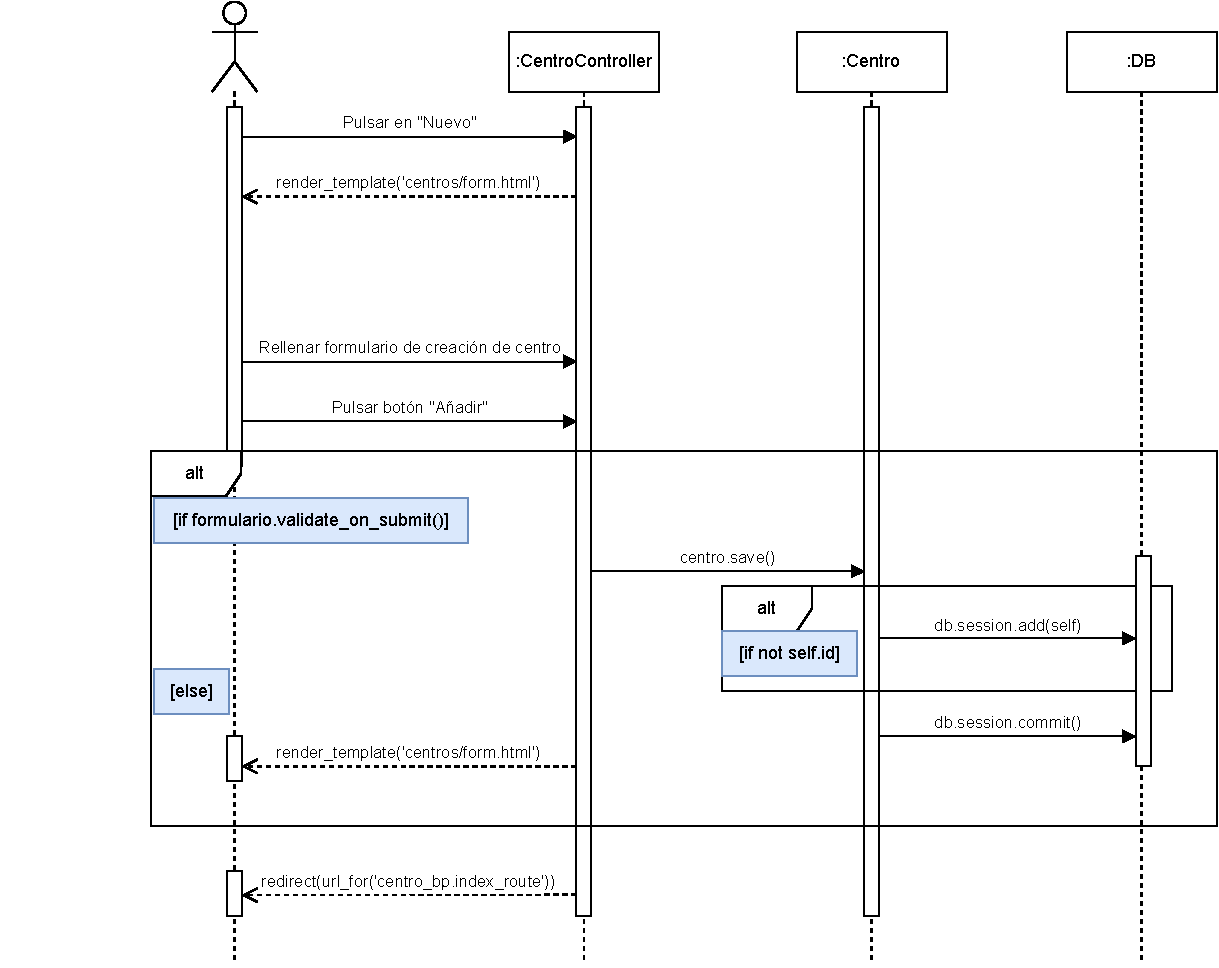
\includegraphics[width=\textwidth]{../img/Anexos/Diagramas secuencia/DS - crear centro.pdf}
	\caption{\textit{Diagrama de secuencia referente a la creación de centros.}}\label{DS-crearCentro}
\end{figure}

\item \textbf{Modificación de centro}

En el diagrama~\ref{DS-modificarCentro} se muestra el proceso seguido para modificar un centro.
Se parte de la base de que el centro ya se encuentra creado.
Al igual que en el caso anterior, este diagrama sirve de ejemplo para la modificación de <<Titulación>>, <<Asignatura>>, <<Docente>>, <<Plaza>>, <<Contrato>>, <<Área>> y <<Departamento>>.

Suponiendo que el usuario se encuentra en la ventana de centros y que ahí por lo menos un centro creado, pulsa en el icono de lápiz de uno de los centros de la lista.

Al realizar esta acción se abre un formulario con los datos del centro seleccionado.
Desde aquí el usuario puede cambiar los campos que quiera.
Una vez realizados los cambios debe pulsar sobre <<Modificar>>.

Una vez modificados los campos y pulsada la opción indicada anteriormente, el servidor recogerá los datos. 
Si todo está bien, las modificaciones se almacenarán en la base de datos y el usuario será redirigido a la ventana principal de los centros.
En caso contrario, se recargará la página del formulario indicando los campos que tienen errores y qué errores son.

\begin{figure}
	\centering
	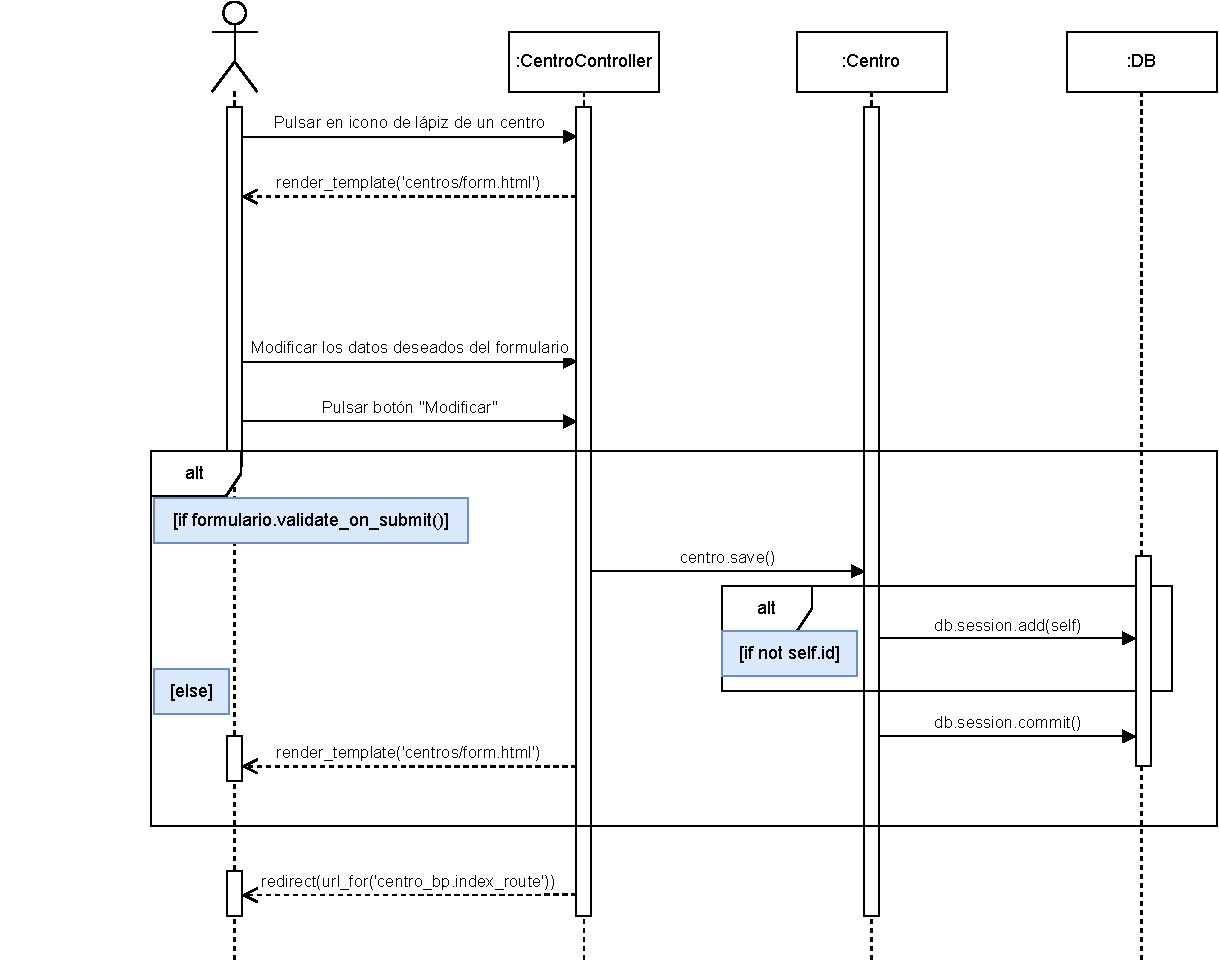
\includegraphics[width=\textwidth]{../img/Anexos/Diagramas secuencia/DS - modificar centro.pdf}
	\caption{\textit{Diagrama de secuencia referente a la modificación de centros.}}\label{DS-modificarCentro}
\end{figure}

\item \textbf{Eliminación de centro}

El diagrama~\ref{DS-eliminarCentro} muestra al secuencia de pasos que se siguen para eliminar un centro de la aplicación.

Partiendo de la base de que existe al menos un centro creado y que el usuario se encuentra en la ventana de centros, el usuario pulsar sobre el icono de una papelera de un centro de la tabla.
Al realizar esta acción aparece una ventana de confirmación para afirmar que se quiere eliminar el centro. 
Al pulsar en aceptar se manda al servidor la petición de eliminación.

En el servidor se comprobará si el centro existe. 
Si no existe se devolverá un error 404 mientras que si existe se comprobará si el centro tiene titulaciones que dependan de él.
En caso afirmativo se redireccionará al usuario a la ventana principal de centros indicando que no se puede eliminar el centro porque tiene titulaciones asociadas.
En caso de que el centro no tenga titulaciones asociadas, se eliminará de la base de datos y se redireccionará al usuario a la vista principal de centros indicando en un mensaje que el centro se ha eliminado correctamente.

\begin{figure}
	\centering
	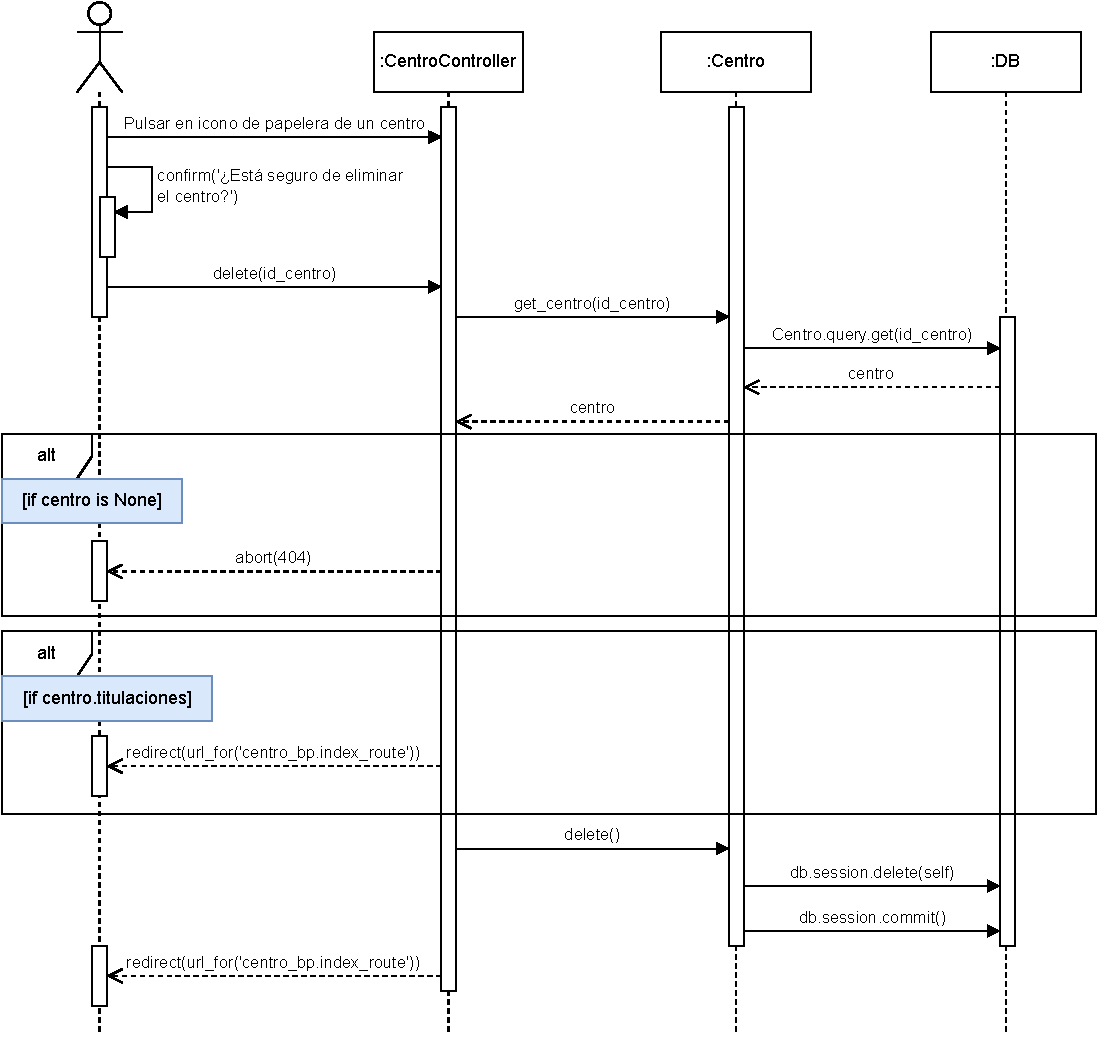
\includegraphics[width=\textwidth]{../img/Anexos/Diagramas secuencia/DS - eliminar centro.pdf}
	\caption{\textit{Diagrama de secuencia de la eliminación de centros.}}\label{DS-eliminarCentro}
\end{figure}

\item \textbf{Asignar plaza a docente}

En el diagrama~\ref{DS-asignarPlaza} se puede ver el conjunto de pasos seguidos para asignar una plaza a un docente.
Para este caso se supone que se tiene una plaza y un docente creados previamente.

El cliente pulsa en el icono del lápiz de una de las plazas.
Esto abre el formulario de edición de la plaza desde donde puede seleccionar el docente a través del campo de búsqueda de docentes escribiendo el nombre del mismo.
Con el docente seleccionado se pulsa en <<Modificar>>.

Si todos los campos del formulario son correctos, se comprueba si el docente tiene alguna plaza sin fecha de cese, en ese caso no se puede vincular con esta plaza y se mostrará un mensaje informando del error. 
En caso contrario, la plaza se asigna.

Finalmente, los cambios se guardan en la base de datos y se redirecciona al usuario a la vista de plazas donde se muestran los mensajes correspondientes a la correcta modificación de la plaza y, si no ha sido posible asignar la plaza por culpa de poseer alguna plaza sin fecha de cese, también se muestra en un mensaje de error.
En caso de no haber pasado la validación del formulario, se redirecciona a la ventana del formulario mostrando los errores detectados.

\begin{figure}
	\centering
	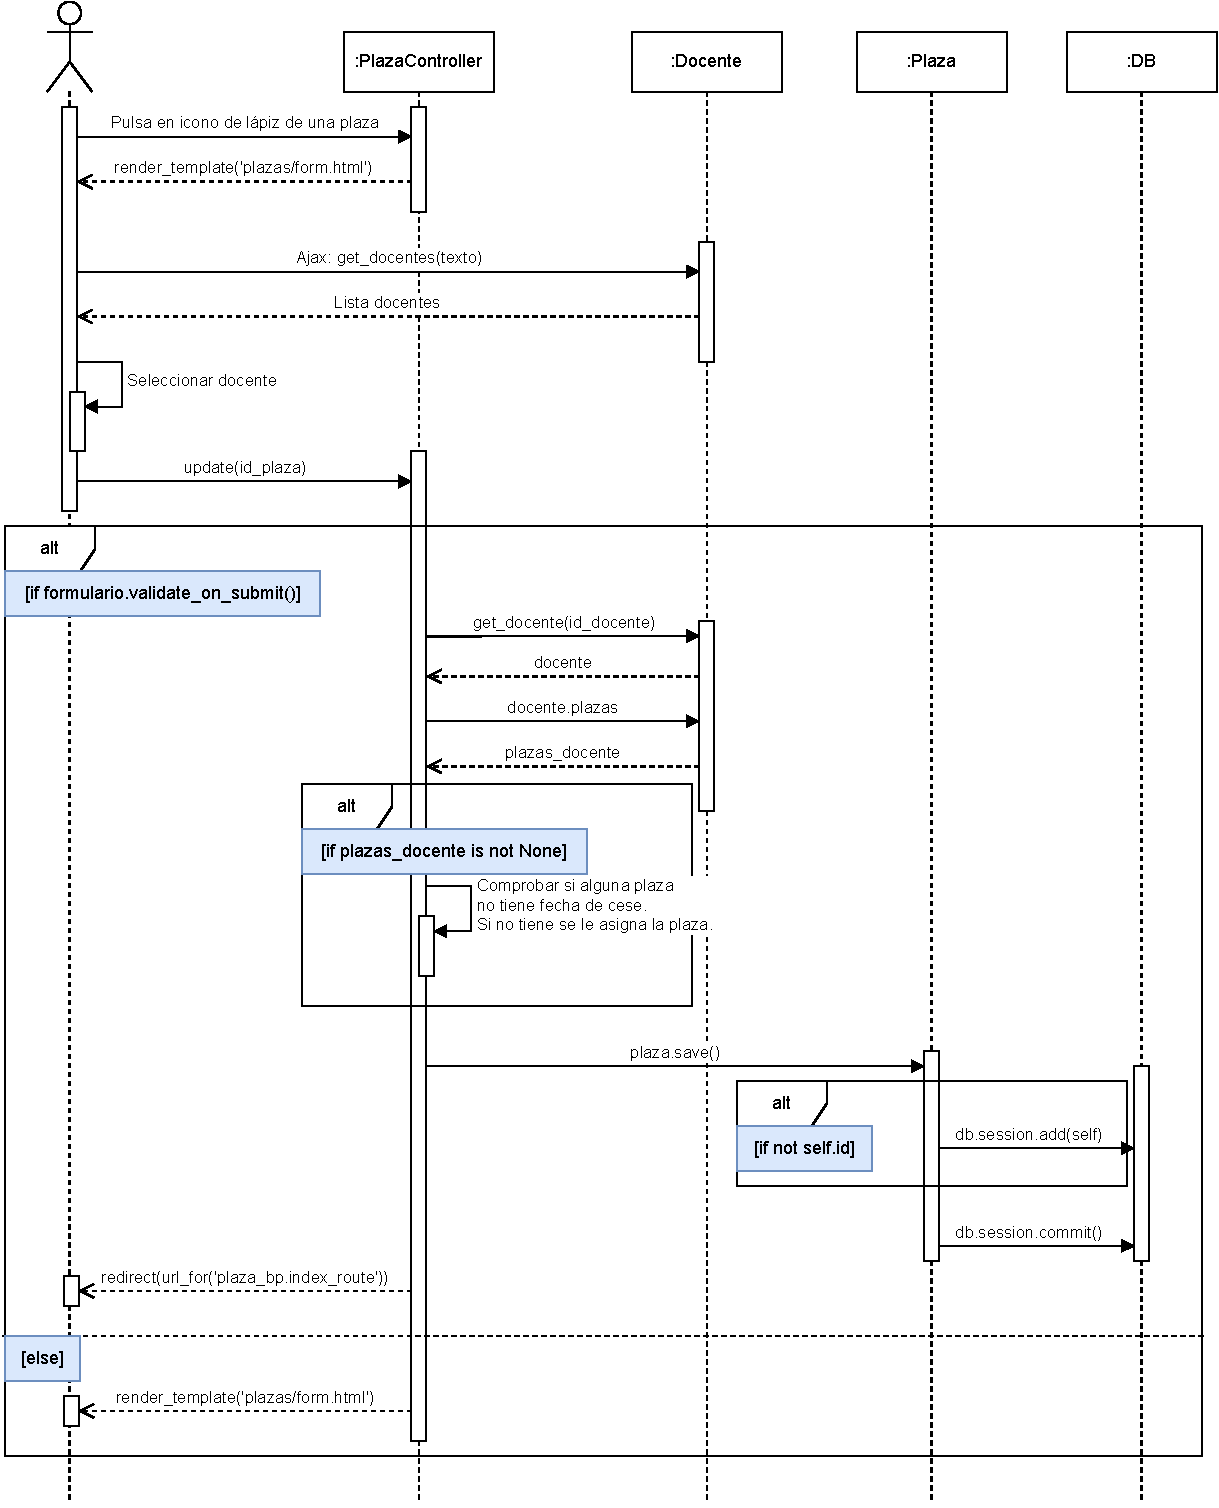
\includegraphics[width=\textwidth]{../img/Anexos/Diagramas secuencia/DS - asignar plaza.pdf}
	\caption{\textit{Diagrama de secuencia de la asignación de una plaza a un docente.}}\label{DS-asignarPlaza}
\end{figure}

\item \textbf{Creación de curso académico}

El diagrama~\ref{DS-crearCurso} contiene los pasos necesarios para crear un nuevo curso académico.

El usuario parte de la ventana de cursos donde debe pulsar sobre <<Nuevo>>. Esto abre una ventana donde se indica el año de inicio del nuevo curso a crear y se pulsa sobre <<Añadir>>.

Con el paso anterior realizado, el usuario se encuentra en la ventana donde puede seleccionar el número de alumnos de cada modalidad y las asignaturas que quiere incluir al curso. Después de realizar la selección deseada pulsa sobre <<Añadir>>. Esto hará que se cree la vinculación entre el curso y aquellas asignaturas que no están ya vinculadas. Además, se crea un grupo de tipo presencial y otro de tipo práctico por cada asignatura.

En caso de producirse algún error con el formulario de introducción de año, como por ejemplo añadir un año de un curso existente, se devolverá al usuario a la ventana del formulario indicando el error. Lo mismo ocurre en el formulario de selección de asignaturas, si el formulario no se valida correctamente, se le mostrará el error al usuario en el propio formulario.

Si al final todo ha ido bien, el usuario será redirigido a la ventana principal de cursos donde podrá ver el curso creado y un mensaje indicando la correcta creación y asignación de asignaturas realizada.


\begin{figure}
	\centering
	\includegraphics[width=\textwidth]{../img/Anexos/Diagramas secuencia/DS - crear curso.pdf}
	\caption{\textit{Diagrama de secuencia de la creación de un curso académico.}}\label{DS-crearCurso}
\end{figure}


\item \textbf{Creación de grupo}

En el diagrama~\ref{DS-crearGrupo} se muestra el proceso seguido para crear un nuevo grupo en una asignatura vinculada a un curso académica. Se parte de la base de que existe un curso con al menos una asignatura y que el usuario se encuentra en la ventana de grupos donde aparece un listado de las asignaturas del curso académico.

El usuario comienza el proceso pulsando sobre el icono de dos personas de una asignatura del listado. De esta manera será redirigido a la vista de los grupos de la asignatura. Acto seguido pulsa sobre el botón <<Añadir grupo>>, lo que abre una ventana modal donde podrá seleccionar entre las modalidades teórico o presencial para el nuevo grupo a crear. Una vez seleccionada esta opción, pulsa sobre el botón <<Añadir>> y la ventana modal se cerrará. Además, aparecerá un mensaje informando de la creación y se podrá ver el grupo en la lista.

\begin{figure}
	\centering
	\includegraphics[width=\textwidth]{../img/Anexos/Diagramas secuencia/DS - crear grupo.pdf}
	\caption{\textit{Diagrama de secuencia de creación de grupos.}}\label{DS-crearGrupo}
\end{figure}

\item \textbf{Asignación de horas de una plaza a un grupo}

El diagrama~\ref{DS-asignarHoras} representa la secuencia seguida para vincular una plaza a un grupo indicando el número de horas de docencia que va a impartir.

Se parte de que el usuario se encuentra en la ventana llamada <<Horas>> y que existe al menos un grupo y una plaza en la aplicación. 

El usuario pulsa sobre el icono del reloj de uno de los grupos de la lista que aparece en la pantalla. Esto abre una nueva ventana donde se pueden ver todos las plazas que cuentan con horas en ese grupo. El usuario pulsa en <<Añadir Plaza>>, lo que abre una ventana modal con un buscador mediante Ajax de la plaza y un campo para indicar las horas. El usuario selecciona una plaza e indica las horas y pulsa en <<Añadir>>.

De forma interna, el controlador de la plaza realiza una búsqueda de la plaza y grupo para asegurarse de que existen, con esta comprobación hecha se recogen las plazas del grupo. 
Si la plaza que se quiere asignar ya se encuentra en ese grupo no se permite, en caso contrario la plaza se vincula con las horas indicadas.

\begin{figure}
	\centering
	\includegraphics[width=\textwidth]{../img/Anexos/Diagramas secuencia/DS - asignar horas.pdf}
	\caption{\textit{Diagrama de secuencia de la asignación de horas de una plaza a un grupo.}}\label{DS-asignarHoras}
\end{figure}

\end{itemize}


\section{Diseño arquitectónico}
El diseño arquitectónico define la estructura del \textit{software} creado respecto a la distribución de las clases y el patrón de diseño utilizado.

En este proyecto se ha seguido la arquitectura cliente-servidor bajo el patrón de diseño Modelo-vista-controlador (MVC).
Flask, que ha sido el \textit{framework} elegido para realizar el código de la aplicación, no obliga al uso de este patrón; sin embargo, se decidió utilizarlo se decidió utilizarlo debido a la organización que proporciona. 
Esto permite que el código quede separado de una forma fácil de entender, de modo que cualquier programador pueda identificar claramente la ubicación de cada elemento.

\begin{itemize}
\item \textbf{Modelo:}
Es el encargado del manejo de los datos de la aplicación.

\item \textbf{Vista:} 
Es la representación de los datos que ve el cliente de la web.
En este caso mediante código HTML bajo el uso del motor de plantillas Jinja2.

\item \textbf{Controlador:} 
Es la parte de la aplicación donde se encuentra la parte importante de la lógica.
Actúa de intermediario entre el cliente y los datos, recogiendo las peticiones de los clientes y haciendo las peticiones necesarias a los modelos para procesar la información requerida y devolver la respuesta al cliente a través de la vista.
\end{itemize}

En el diagrama~\ref{MVC} se representa el funcionamiento del MVC donde el usuario de la web interacciona, a través de la vista, con el controlador que se encarga de hacer peticiones y respuestas de datos con el modelo.
De esta forma el controlador es capaz de recuperar, modificar o eliminar los datos de un modelo.
Además, el controlador es el encargado de formar el código necesario para mostrar la vista que visualizará el usuario de la web.


\begin{figure}
	\centering
	\includegraphics[width=\textwidth]{../img/Anexos/MVC.pdf}
	\caption{\textit{Modelo-Vista-Controlador}}\label{MVC}
\end{figure}







\apendice{Documentación técnica de programación}

\section{Introducción}
En este anexo se muestra toda la información necesaria para que un desarrollador pueda poner en funcionamiento el \textit{software} de este proyecto.
Además, se da una explicación sobre la estructura del código y aquellos aspectos que puedan ser importantes para cualquier desarrollador que vea por primera vez el código desarrollado.

\section{Estructura de directorios}
La estructura de los directorios del proyecto es la siguiente:
\begin{itemize}
\item \textbf{docs:} Contiene la documentación del proyecto.
\item \textbf{src:} Dentro de este directorio se encuentra el código fuente del proyecto desarrollado.
\end{itemize}

Este anexo va a centrarse en la explicación del contenido del directorio \texttt{src}.
En la figura~\ref{fig:directorios} se puede ver la distribución de los directorios que se encuentran dentro de \texttt{src}.

\begin{figure}
	\centering
	\includegraphics[width=\textwidth]{../img/Anexos/directorios.pdf}
	\caption{\textit{Directorios del proyecto}}\label{fig:directorios}
\end{figure}

A continuación se da una explicación de lo contenido en cada directorio:
\begin{itemize}
\item \texttt{src:} 
Es el directorio principal del código fuente del proyecto que contiene a todos los demás. 
Además, en su interior se encuentra el fichero \texttt{app.py} desde el que se carga la configuración y se arranca la aplicación, el fichero \texttt{forms.py} que contiene todos los formularios generados a partir de al biblioteca WTForms y el fichero \texttt{decorators.py} que contiene aquellas funciones encargadas de detectar los permisos del usuario activo y su \textit{token}.
Por otro lado, también se encuentran los ficheros \texttt{Procfile} necesario para desplegar la aplicación en Heroku, \texttt{requirements.txt} que contiene todas las bibliotecas junto a su versión requerida y el fichero \texttt{runtime.txt} también necesario para desplegar en Heroku donde se indica la versión de Python.

\item \texttt{config:} 
Contiene tres ficheros necesarios para la configuración del proyecto.
El fichero \texttt{config.py} indica la configuración general del proyecto mientras que los ficheros \texttt{development.py} y \texttt{production.py} contienen la configuración necesaria para el despliegue en modo desarrollo y modo producción respectivamente.

\item \texttt{controllers:}
En este directorio se encuentran todos los controladores del proyecto.

\item \texttt{migrations:}
Es un directorio perteneciente a la librería Flask-Migrate. 
Este directorio es utilizado para almacenar la configuración de la biblioteca y las diferentes migraciones creadas para actualizar la base de datos evitando la pérdida de información almacenada. (En principio, no sería necesario modificar nada de este directorio).

\item \texttt{models:}
Aquí se encuentran todos los ficheros respectivos a los modelos de la aplicación web. Es decir, aquellos objetos que se crean y almacenan en la aplicación.
Desde cada uno de estos ficheros también se define la estructura de sus tablas en la base de datos.

\item \texttt{routes:}
Este directorio almacena los diferentes ficheros que definen las rutas de la aplicación, organizadas por \textit{blueprints}.

En estos ficheros se indican los decoradores de cada ruta y la acción del controlador asociada que se debe ejecutar con la petición a esa ruta. 
Además, se define el tipo de petición HTTP permitida por ruta.

\item \texttt{static:} 
Como su nombre indica, este directorio contiene todos aquellos ficheros estáticos de la aplicación que van a ser cargados por las vistas. 
Los ficheros que contiene son accesibles desde un navegador y aquí se almacenan imágenes, ficheros CSS, ficheros de JavaScript y las librerías de JavaScript cargadas desde el sistema de gestión de paquetes NPM, junto al fichero de configuración donde se indican las bibliotecas y su versión llamado \texttt{package.json}.

\item \texttt{templates:}
Este directorio agrupa todas aquellas vistas de la aplicación web.
Dentro se encuentra dividido a su vez por otros directorios con el nombre de los diferentes modelos para tener más organizadas las vistas.

En este directorio también se encuentra el fichero \texttt{base\_template.html} que define la plantilla base de todas las demás vistas.
Desde este fichero se define la carga de los ficheros CSS y \textit{scripts} de JavaScript, además de otros elementos como el menú de la aplicación.

En este fichero todos los elementos se encuentran divididos por bloques para cargar solo aquellos necesarios.
Por ejemplo, el footer solo se carga en la vista de \textit{login}, pero el bloque de carga se define aquí.

\item \texttt{utils:}
Este directorio está creado para mejorar la carga y organización de la aplicación.
Dentro del directorio se encuentra el fichero \texttt{db.py} donde se cargan las bibliotecas relativas a la base de datos como SQLAlchemy o Flask-Migrate.
\end{itemize}

\section{Manual del programador}
En esta sección se van exponer algunos detalles necesarios para el entendimiento del código desarrollado teniendo en cuenta la explicación de la estructura de directorios dada en la sección anterior.

Como se ha comentado antes, los archivos necesarios para la configuración del proyecto se encuentran dentro del directorio \texttt{config}.

El fichero \texttt{config.py} contiene la configuración general del proyecto. En la la figura~\ref{fig:ficheroConfig} se muestra el contenido del fichero. En él se puede ver como se indica la clave secreta junto a otras configuraciones como el modo \textit{debug}, las sesiones, el \textit{email} del administrador, etc.

\begin{figure}
	\centering
	\includegraphics[width=\textwidth]{../img/Anexos/ManualProgramador/config.png}
	\caption{\textit{Fichero config.py}}\label{fig:ficheroConfig}
\end{figure}

En la figura~\ref{fig:ficheroDev} se puede ver el fichero \texttt{development.py}. 
En este fichero se activa el modo \textit{debug} y se indica cual va a ser la base de datos. 
La configuración de este fichero sólo se cargará si en el sistema se encuentra la variable de entorno \texttt{FLASK\_ENV}. 
Esta carga se puede ver en el fichero \texttt{app.py}. 
Por defecto se utiliza el valor \texttt{development}, por lo que si la variable no está definida se tomará la configuración de desarrollo.

\begin{figure}
	\centering
	\includegraphics[width=\textwidth]{../img/Anexos/ManualProgramador/development.png}
	\caption{\textit{Fichero development.py}}\label{fig:ficheroDev}
\end{figure}

Por último, en la figura~\ref{fig:ficheroProd} se muestra la configuración del proyecto para el caso de tener el entorno definido como producción.

En este caso la ruta de la base de datos se obtiene desde una variable de entorno llamada \texttt{JAWSDB\_MARIA\_URL} que debe encontrarse definida en el sistema.

Este nombre puede cambiarse sin problema, pero se le dio este nombre debido a que en Heroku, plataforma donde se ha desplegado la aplicación, tiene ese nombre la variable.

\begin{figure}
	\centering
	\includegraphics[width=\textwidth]{../img/Anexos/ManualProgramador/production.png}
	\caption{\textit{Fichero production.py}}\label{fig:ficheroProd}
\end{figure}


\section{Compilación, instalación y ejecución del proyecto}
En esta sección se van a especificar los pasos que se deben seguir para poder desplegar la aplicación de forma correcta para poder ser utilizada.

Lo primero y más importante es conseguir el código fuente. 
Este se puede descargar desde el repositorio\footnote{\url{https://github.com/idg0015/Aplicacion-de-gestion-del-PDI-de-un-area-de-la-UBU}} del proyecto.

Para realizar la descarga se puede utilizar la opción de GitHub de descargar desde la página web mediante un archivo ZIP o utilizar Git para realizar una clonación del repositorio mediante el comando \texttt{git clone}.

\subsection{Preparación del entorno}
Para el desarrollo de la aplicación se ha utilizado el IDE PyCharm y se recomienda su uso ya que aligera el proceso de preparación del entorno al contener perfiles ya pre-creados para distintos \textit{frameworks} siendo uno de ellos Flask.

De todas forma, en caso contrario, para preparar el entorno de trabajo lo primero que se debe instalar en el sistema es Python.
Esto se puede realizar mediante una descarga de su web\footnote{Se puede descargar desde aquí: \url{https://www.python.org/downloads/}} y seguir los pasos del instalador. Para este proyecto se ha utilizado Python 3.9.

También se debe instalar algún sistema gestor de bases de datos como MariaDB o MySQL.

Con Python instalado, lo recomendable es crear un entorno virtual para ejecutar Python, de esta manera se pueden tener diferentes versiones de Python instaladas y, según el entorno, ejecutar una u otra.
Para ello, se debe ejecutar el comando \texttt{virtualenv env} para crear el entorno y acto seguido ejecutar \texttt{env\textbackslash{}Scripts\textbackslash{}activate.bat} (en el caso de Windows) para indicar que queremos utilizar el entorno.
Esto hará que en el \textit{prompt} de la consola aparezca la palabra <<(env)>>, lo que nos asegurará de que estamos trabajando bajo el entorno.

Por último, en la raíz del proyecto se debe ejecutar el comando \texttt{pip install -r requirements.txt}.
De esta forma quedarán instaladas las bibliotecas necesarias para Python.

Para instalar las bibliotecas de JavaScript necesarias para el uso de la aplicación se debe ejecutar el comando \texttt{npm i} a nivel de carpeta \texttt{src/static}, donde se encuentra el archivo <<package.json>> en el que se indican las bibliotecas a descargar junto a su versión. 

Con todo esto realizado ya tendríamos configurado lo necesario para poder arrancar la aplicación.
Para ello se deben seguir los siguientes pasos:
\begin{enumerate}
\item Ejecutar el comando \texttt{export FLASK\_APP=app.py} para exportar la variable de entorno que indica el fichero desde el que arranca la aplicación.
\item Se podría hacer lo mismo para FLASK\_ENV y FLASK\_DEBUG con los valores <<development>> y <<1>> respectivamente para su uso en desarrollo, pero no debería ser algo necesario ya que esto se encuentra en los ficheros de configuración de la aplicación.
\item Ejecutar el comando \texttt{python -m flask run}.
\end{enumerate}

Con esto realizado la aplicación habría arrancado y al acceder a la dirección <<127.0.0.1:5000>> debería verse la aplicación.
En este paso lo único que necesario para poder acceder al contenido de la aplicación es almacenar un docente en la base de datos desde el sistema gestor utilizado que tenga como correo electrónico el mismo utilizado para iniciar sesión en el Moodle de una universidad.

\subsection{Despliegue en Heroku}
En este apartado se va a dar la explicación para desplegar la aplicación web en la plataforma Heroku.

En primer lugar es necesario tener los ficheros <<requirements.txt>>, <<runtime.txt>>, <<Procfile>> y <<package.json>> a nivel de la raíz del directorio a subir, ya que si no Heroku no será capaz de poder utilizarlos (estos archivos ya se encuentran incluidos en el repositorio).

Es importante saber que el fichero <<package.json>> no debe ser el mismo que se encuentra en el directorio <<static>>, donde se indican los paquetes a instalar, si no que debe ser un fichero que apunte a este otro, desde donde sí se hará la instalación. 
Esto es debido a que Heroku no es capaz de detectar el archivo <<package.json>> si se encuentra dentro del directorio <<static>>. Además, si ponemos el fichero tal cual, los paquetes se instalaran en la raíz del proyecto y no en la carpeta static.

El contenido del fichero <<package.json>> en la raíz del proyecto debería ser algo parecido a lo mostrado en la figura~\ref{fig:ficheroPackage}.

Como se puede ver, cuenta con una instrucción <<\textit{postinstall}>> donde se indica que se mueva al directorio <<static>> y ahí haga la instalación de paquetes.
Cuando se haga el \texttt{npm install} consultará el fichero <<package.json>> de la carpeta <<static>>.

\begin{figure}
	\centering
	\includegraphics[width=.8\textwidth]{../img/Anexos/ManualProgramador/package.png}
	\caption{\textit{Fichero package.json de la raíz del proyecto}}\label{fig:ficheroPackage}
\end{figure}


\section{Pruebas del sistema}
En esta sección se van a realizar distintas pruebas para asegurar que el \textit{software} desarrollado funciona de la forma esperada y para corregir los fallos en caso contrario.

\subsection{Casos de prueba}
A continuación se presentan todos los casos de prueba realizados.

\begin{table}[H]
\begin{tabular}{p{.17\textwidth} p{.12\textwidth} p{.2\textwidth} p{.2\textwidth} p{.14\textwidth}}
\cellcolor{gray!25}
ID   & CP1 & \cellcolor{gray!25} Prioridad   & Alta \\ \hline
\cellcolor{gray!25} Fecha	&	\multicolumn{4}{l}{26/06/2023} \\ \hline
\cellcolor{gray!25} Descripción		&	\multicolumn{4}{l}{Probar el inicio de sesión correcto de la aplicación} \\ \hline                                            
\cellcolor{gray!25}
Precondición  & \multicolumn{4}{l}{No tener sesión iniciada} \\ \hline
\cellcolor{gray!25} Postcondición & \multicolumn{4}{l}{No hay sesión iniciada}                                                                                                      \\ \hline
\rowcolor{gray!25}
\textbf{Paso}   & \textbf{Entrada} & \textbf{Salida esperada} & \textbf{Salida real} & \textbf{Resultado} \\ \hline
Acceder a la página de \textit{login} 
& \texttt{/login}                                                                             
& Redirección a la página de \textit{login}                                    
& Redirección a la página de \textit{login}                                   
& Correcto                            
\\ \hline
Rellenar formulario de inicio de sesión
& Email: idg0015-
@alu.ubu.-
es, Contraseña: XXXX                                                                                                        
& Datos introducidos                               
& Datos introducidos                                
& Correcto                            
\\ \hline
Iniciar sesión
& Hacer clic en <<Iniciar sesión>>
& Redirección a la página principal                                 
& Redirección a la página principal                                 
& Correcto                            
\\ \hline                 
\end{tabular}
\caption{Caso de prueba 1: Inicio de sesión correcto.}
\end{table}

\begin{table}[H]
\begin{tabular}{p{.17\textwidth} p{.12\textwidth} p{.2\textwidth} p{.2\textwidth} p{.14\textwidth}}
\cellcolor{gray!25}
ID   & CP2 & \cellcolor{gray!25} Prioridad   & Alta \\ \hline
\cellcolor{gray!25} Fecha	&	\multicolumn{4}{l}{26/06/2023} \\ \hline
\cellcolor{gray!25} Descripción		&	\multicolumn{4}{l}{Probar el inicio de sesión fallido de la aplicación} \\ \hline                                            
\cellcolor{gray!25}
Precondición  & \multicolumn{4}{l}{No tener sesión iniciada} \\ \hline
\cellcolor{gray!25} Postcondición & \multicolumn{4}{l}{No hay sesión iniciada}                                                    \\ \hline
\rowcolor{gray!25}
\textbf{Paso}   & \textbf{Entrada} & \textbf{Salida esperada} & \textbf{Salida real} & \textbf{Resultado} \\ \hline
Acceder a la página de \textit{login} 
& \texttt{/login}                                                                             
& Redirección a la página de \textit{login}                                    
& Redirección a la página de \textit{login}                                   
& Correcto                            
\\ \hline
Rellenar formulario de inicio de sesión
& Email: test@-
gmail.com, Contraseña: 1234
& Datos introducidos                               
& Datos introducidos                               
& Correcto                            
\\ \hline
Iniciar sesión
& Hacer clic en <<Iniciar sesión>>
& Mensaje: ``Usuario o contraseña incorrectos''
& Mensaje: ``Usuario o contraseña incorrectos''
& Correcto                            
\\ \hline                 
\end{tabular}
\caption{Caso de prueba 2: Inicio de sesión fallido.}
\end{table}

\begin{table}[H]
\begin{tabular}{p{.17\textwidth} p{.12\textwidth} p{.2\textwidth} p{.2\textwidth} p{.14\textwidth}}
\cellcolor{gray!25}
ID   & CP3 & \cellcolor{gray!25} Prioridad   & Alta \\ \hline
\cellcolor{gray!25} Fecha	&	\multicolumn{4}{l}{26/06/2023} \\ \hline
\cellcolor{gray!25} Descripción		&	\multicolumn{4}{l}{Probar la correcta creación de un centro} \\ \hline                                            
\cellcolor{gray!25}
Precondición  & \multicolumn{4}{l}{Tener sesión iniciada con permisos de modificación} \\ \hline
\cellcolor{gray!25} Postcondición & \multicolumn{4}{l}{No hay sesión iniciada}                                                    \\ \hline
\rowcolor{gray!25}
\textbf{Paso}   & \textbf{Entrada} & \textbf{Salida esperada} & \textbf{Salida real} & \textbf{Resultado} \\ \hline
Acceder a la página de centros 
& \texttt{/centros}                                                                             
& Redirección a la página de centros                                   
& Redirección a la página de centros                                   
& Correcto                            
\\ \hline
Abrir formulario de ingreso
& Clic en <<Nuevo>>
& Redirección a \texttt{/centros/nuevo}                               
& Redirección a \texttt{/centros/nuevo}                              
& Correcto                            
\\ \hline
Rellenar formulario de ata de centro
& Código interno: 13, Nombre: Escuela Politécnica Superior, Río Vena, Abreviatura: EPSv, Email del administrativo: departamentos.eps@ubu.es
& Datos introducidos                               
& Datos introducidos                               
& Correcto                            
\\ \hline
Crear centro
& Hacer clic en <<Añadir>>
& Mensaje: ``Centro añadido correctamente''. Redirección a \texttt{/centros}
& Mensaje: ``Centro añadido correctamente''. Redirección a \texttt{/centros}
& Correcto                            
\\ \hline                 
\end{tabular}
\caption{Caso de prueba 3: Creación correcta de centro.}
\end{table}

\begin{table}[H]
\begin{tabular}{p{.17\textwidth} p{.12\textwidth} p{.2\textwidth} p{.2\textwidth} p{.14\textwidth}}
\cellcolor{gray!25}
ID   & CP4 & \cellcolor{gray!25} Prioridad   & Media \\ \hline
\cellcolor{gray!25} Fecha	&	\multicolumn{4}{l}{26/06/2023} \\ \hline
\cellcolor{gray!25} Descripción		&	\multicolumn{4}{l}{Creación de un centro faltando campos obligatorios} \\ \hline                                            
\cellcolor{gray!25}
Precondición  & \multicolumn{4}{l}{Tener sesión iniciada con permisos de modificación} \\ \hline
\cellcolor{gray!25} Postcondición & \multicolumn{4}{l}{No hay sesión iniciada}                                                    \\ \hline
\rowcolor{gray!25}
\textbf{Paso}   & \textbf{Entrada} & \textbf{Salida esperada} & \textbf{Salida real} & \textbf{Resultado} \\ \hline
Acceder a la página de centros 
& \texttt{/centros}                                                                             
& Redirección a la página de centros                                   
& Redirección a la página de centros                                   
& Correcto                            
\\ \hline
Abrir formulario de ingreso
& Clic en <<Nuevo>>
& Redirección a \texttt{/centros/nuevo}                               
& Redirección a \texttt{/centros/nuevo}                              
& Correcto                            
\\ \hline
Rellenar formulario de ata de centro
& Código interno: 13, Abreviatura: EPSv, Email del administrativo: departamentos.eps@ubu.es
& Datos introducidos                               
& Datos introducidos                               
& Correcto                            
\\ \hline
Crear centro
& Hacer clic en <<Añadir>>
& Mensaje: ``El nombre es obligatorio''
& Mensaje: ``El nombre es obligatorio''
& Correcto                            
\\ \hline                 
\end{tabular}
\caption{Caso de prueba 4: Creación de un centro faltando campos obligatorios.}
\end{table}

\begin{table}[H]
\begin{tabular}{p{.17\textwidth} p{.12\textwidth} p{.2\textwidth} p{.2\textwidth} p{.14\textwidth}}
\cellcolor{gray!25}
ID   & CP5 & \cellcolor{gray!25} Prioridad   & Media \\ \hline
\cellcolor{gray!25} Fecha	&	\multicolumn{4}{l}{26/06/2023} \\ \hline
\cellcolor{gray!25} Descripción		&	\multicolumn{4}{l}{Eliminación de un centro sin titulaciones vinculadas} \\ \hline                                            
\cellcolor{gray!25}
Precondición  & \multicolumn{4}{p{.66\textwidth}}{Tener sesión iniciada con permisos de modificación y tener un centro creado sin titulaciones vinculadas} \\ \hline
\cellcolor{gray!25} Postcondición & \multicolumn{4}{l}{No hay sesión iniciada}                                                    \\ \hline
\rowcolor{gray!25}
\textbf{Paso}   & \textbf{Entrada} & \textbf{Salida esperada} & \textbf{Salida real} & \textbf{Resultado} \\ \hline
Acceder a la página de centros 
& \texttt{/centros}                                                                             
& Redirección a la página de centros                                   
& Redirección a la página de centros                                   
& Correcto                            
\\ \hline
Eliminar un centro
& Clic en icono de papelera de un centro de la tabla
& Alerta: ``¿Está seguro de eliminar el centro? No se podrá eliminar si tiene alguna titulación vinculada''
& Alerta: ``¿Está seguro de eliminar el centro? No se podrá eliminar si tiene alguna titulación vinculada''                              
& Correcto
\\ \hline
Aceptar la alerta
& Clic en <<Aceptar>>
& Mensaje: ``Centro eliminado correctamente''                              
& Mensaje: ``Centro eliminado correctamente''                             
& Correcto                            
\\ \hline                
\end{tabular}
\caption{Caso de prueba 5: Eliminación de un centro sin titulaciones vinculadas.}
\end{table}

\begin{table}[H]
\begin{tabular}{p{.17\textwidth} p{.12\textwidth} p{.2\textwidth} p{.2\textwidth} p{.14\textwidth}}
\cellcolor{gray!25}
ID   & CP6 & \cellcolor{gray!25} Prioridad   & Alta \\ \hline
\cellcolor{gray!25} Fecha	&	\multicolumn{4}{l}{26/06/2023} \\ \hline
\cellcolor{gray!25} Descripción		&	\multicolumn{4}{l}{Eliminación de un centro con titulaciones vinculadas} \\ \hline                                            
\cellcolor{gray!25}
Precondición  & \multicolumn{4}{p{.66\textwidth}}{Tener sesión iniciada con permisos de modificación y tener un centro creado con titulaciones vinculadas} \\ \hline
\cellcolor{gray!25} Postcondición & \multicolumn{4}{l}{No hay sesión iniciada}                                                    \\ \hline
\rowcolor{gray!25}
\textbf{Paso}   & \textbf{Entrada} & \textbf{Salida esperada} & \textbf{Salida real} & \textbf{Resultado} \\ \hline
Acceder a la página de centros 
& \texttt{/centros}                                                                             
& Redirección a la página de centros                                   
& Redirección a la página de centros                                   
& Correcto                            
\\ \hline
Eliminar un centro
& Clic en icono de papelera de un centro de la tabla
& Alerta: ``¿Está seguro de eliminar el centro? No se podrá eliminar si tiene alguna titulación vinculada''
& Alerta: ``¿Está seguro de eliminar el centro? No se podrá eliminar si tiene alguna titulación vinculada''                              
& Correcto
\\ \hline
Aceptar la alerta
& Clic en <<Aceptar>>
& Mensaje: ``No se puede eliminar el centro porque tiene titulaciones asociadas''                              
& Mensaje: ``No se puede eliminar el centro porque tiene titulaciones asociadas''                             
& Correcto                            
\\ \hline                
\end{tabular}
\caption{Caso de prueba 6: Eliminación de un centro con titulaciones vinculadas.}
\end{table}

\begin{table}[H]
\begin{tabular}{p{.17\textwidth} p{.12\textwidth} p{.2\textwidth} p{.2\textwidth} p{.14\textwidth}}
\cellcolor{gray!25}
ID   & CP7 & \cellcolor{gray!25} Prioridad   & Alta \\ \hline
\cellcolor{gray!25} Fecha	&	\multicolumn{4}{l}{26/06/2023} \\ \hline
\cellcolor{gray!25} Descripción		&	\multicolumn{4}{l}{Creación de una titulación} \\ \hline                                            
\cellcolor{gray!25}
Precondición  & \multicolumn{4}{p{.66\textwidth}}{Tener sesión iniciada con permisos de modificación y tener un centro creado} \\ \hline
\cellcolor{gray!25} Postcondición & \multicolumn{4}{l}{No hay sesión iniciada}                                                    \\ \hline
\rowcolor{gray!25}
\textbf{Paso}   & \textbf{Entrada} & \textbf{Salida esperada} & \textbf{Salida real} & \textbf{Resultado} \\ \hline
Acceder a la página de centros 
& /titulacio-
nes                                                                           
& Redirección a la página de titulaciones                                   
& Redirección a la página de titulaciones                                   
& Correcto                            
\\ \hline
Abrir formulario
& Clic en <<Nuevo>>
& Redirección a /titulaciones/nuevo
& Redirección a /titulaciones/nuevo
& Correcto
\\ \hline
Rellenar formulario
& Código interno: 63, Nombre: Gº en Ing, Informática, Abreviatura: GºII, URL: https://www.ubu.es/grado-en-ingenieria-informatica, Centro: Escuela Politécnica Superior, Río Vena
& Datos introducidos                            
& Datos introducidos
& Correcto                            
\\ \hline   
Crear titulación
& Clic en <<Añadir>>
& Mensaje: ``Tiulación añadida correctamente''                            
& Mensaje: ``Tiulación añadida correctamente''
& Correcto                            
\\ \hline              
\end{tabular}
\caption{Caso de prueba 7: Creación de una titulación.}
\end{table}

\begin{table}[H]
\begin{tabular}{p{.17\textwidth} p{.12\textwidth} p{.2\textwidth} p{.2\textwidth} p{.14\textwidth}}
\cellcolor{gray!25}
ID   & CP8 & \cellcolor{gray!25} Prioridad   & Alta \\ \hline
\cellcolor{gray!25} Fecha	&	\multicolumn{4}{l}{26/06/2023} \\ \hline
\cellcolor{gray!25} Descripción		&	\multicolumn{4}{p{.66\textwidth}}{Eliminación de una titulación sin asignaturas vinculadas} \\ \hline                                            
\cellcolor{gray!25}
Precondición  & \multicolumn{4}{p{.66\textwidth}}{Tener sesión iniciada con permisos de modificación y tener una titulación creada} \\ \hline
\cellcolor{gray!25} Postcondición & \multicolumn{4}{l}{No hay sesión iniciada}                                                    \\ \hline
\rowcolor{gray!25}
\textbf{Paso}   & \textbf{Entrada} & \textbf{Salida esperada} & \textbf{Salida real} & \textbf{Resultado} \\ \hline
Acceder a la página de centros 
& /titulacio-
nes                                                                           
& Redirección a la página de titulaciones                                   
& Redirección a la página de titulaciones                                   
& Correcto                            
\\ \hline
Eliminar titulación
& Clic en el icono de la papelera de una titulación
& Alerta: ``¿Está seguro de eliminar la titulación?''
& Alerta: ``¿Está seguro de eliminar la titulación?''
& Correcto
\\ \hline
Aceptar alerta
& Clic en <<Aceptar>>
& Mensaje: ``Titulación eliminada correctamente''                            
& Mensaje: ``Titulación eliminada correctamente''
& Correcto                            
\\ \hline                
\end{tabular}
\caption{Caso de prueba 8: Eliminación de una titulación sin asignaturas vinculadas.}
\end{table}

\begin{table}[H]
\begin{tabular}{p{.17\textwidth} p{.12\textwidth} p{.2\textwidth} p{.2\textwidth} p{.14\textwidth}}
\cellcolor{gray!25}
ID   & CP9 & \cellcolor{gray!25} Prioridad   & Alta \\ \hline
\cellcolor{gray!25} Fecha	&	\multicolumn{4}{l}{26/06/2023} \\ \hline
\cellcolor{gray!25} Descripción		&	\multicolumn{4}{p{.66\textwidth}}{Eliminación de una titulación con asignaturas vinculadas} \\ \hline                                            
\cellcolor{gray!25}
Precondición  & \multicolumn{4}{p{.66\textwidth}}{Tener sesión iniciada con permisos de modificación y tener una titulación creada con asignaturas vinculadas} \\ \hline
\cellcolor{gray!25} Postcondición & \multicolumn{4}{l}{No hay sesión iniciada}                                                    \\ \hline
\rowcolor{gray!25}
\textbf{Paso}   & \textbf{Entrada} & \textbf{Salida esperada} & \textbf{Salida real} & \textbf{Resultado} \\ \hline
Acceder a la página de centros 
& /titulacio-
nes                                                                           
& Redirección a la página de titulaciones                                   
& Redirección a la página de titulaciones                                   
& Correcto                            
\\ \hline
Eliminar titulación
& Clic en el icono de la papelera de una titulación
& Alerta: ``¿Está seguro de eliminar la titulación? Se eliminarán sus asignaturas asociadas y todo lo que dependa de estas.''
& Alerta: ``¿Está seguro de eliminar la titulación? Se eliminarán sus asignaturas asociadas y todo lo que dependa de estas.''
& Correcto
\\ \hline
Aceptar alerta
& Clic en <<Aceptar>>
& Mensaje: ``No se puede eliminar la titulación porque tiene asignaturas asociadas''                            
& Mensaje: ``No se puede eliminar la titulación porque tiene asignaturas asociadas''
& Correcto                            
\\ \hline                
\end{tabular}
\caption{Caso de prueba 9: Eliminación de una titulación con asignaturas vinculadas.}
\end{table}

\begin{table}[H]
\begin{tabular}{p{.17\textwidth} p{.13\textwidth} p{.2\textwidth} p{.2\textwidth} p{.14\textwidth}}
\cellcolor{gray!25}
ID   & CP10 & \cellcolor{gray!25} Prioridad   & Alta \\ \hline
\cellcolor{gray!25} Fecha	&	\multicolumn{4}{l}{26/06/2023} \\ \hline
\cellcolor{gray!25} Descripción		&	\multicolumn{4}{l}{Creación de una asignatura} \\ \hline                                            
\cellcolor{gray!25}
Precondición  & \multicolumn{4}{p{.66\textwidth}}{Tener sesión iniciada con permisos de modificación y tener una titulación creada} \\ \hline
\cellcolor{gray!25} Postcondición & \multicolumn{4}{l}{No hay sesión iniciada}                                                    \\ \hline
\rowcolor{gray!25}
\textbf{Paso}   & \textbf{Entrada} & \textbf{Salida esperada} & \textbf{Salida real} & \textbf{Resultado} \\ \hline
Acceder a la página de asignaturas 
& /asignatu-
ras                                                                           
& Redirección a la página de asignaturas                                   
& Redirección a la página de asignaturas                                   
& Correcto                            
\\ \hline
Abrir formulario de creación
& Clic en <<Nuevo>>
& Redirección a /asignaturas/nuevo
& Redirección a /asignaturas/nuevo
& Correcto
\\ \hline
Rellenar formulario
& Código interno: 13, Nombre: Programación, Tipo:Formación Básica, Abreviatura: PR, Créditos teoría: 3, Créditos práctica: 3, Curso: 1º, Semestre: 2º, Titulación: Gº en Ing, Informática
& Datos introducidos                           
& Datos introducidos 
& Correcto                            
\\ \hline  
Crear asignatura
& Clic en <<Añadir>>
& Mensaje: ``Asignatura creada correctamente''        
& Mensaje: ``Asignatura creada correctamente''
& Correcto                            
\\ \hline              
\end{tabular}
\caption{Caso de prueba 10: Creación de una asignatura.}
\end{table}

\begin{table}[H]
\begin{tabular}{p{.17\textwidth} p{.13\textwidth} p{.2\textwidth} p{.2\textwidth} p{.14\textwidth}}
\cellcolor{gray!25}
ID   & CP11 & \cellcolor{gray!25} Prioridad   & Alta \\ \hline
\cellcolor{gray!25} Fecha	&	\multicolumn{4}{l}{26/06/2023} \\ \hline
\cellcolor{gray!25} Descripción		&	\multicolumn{4}{l}{Eliminación de una asignatura} \\ \hline                                            
\cellcolor{gray!25}
Precondición  & \multicolumn{4}{p{.66\textwidth}}{Tener sesión iniciada con permisos de modificación y tener una asignatura creada} \\ \hline
\cellcolor{gray!25} Postcondición & \multicolumn{4}{l}{No hay sesión iniciada}                                                    \\ \hline
\rowcolor{gray!25}
\textbf{Paso}   & \textbf{Entrada} & \textbf{Salida esperada} & \textbf{Salida real} & \textbf{Resultado} \\ \hline
Acceder a la página de asignaturas 
& /asignatu-
ras                                                                           
& Redirección a la página de asignaturas                                   
& Redirección a la página de asignaturas                                   
& Correcto                            
\\ \hline
Eliminar asignatura
& Clic en el icono de la papelera de una asignatura
& Alerta: ``¿Está seguro de eliminar la asignatura? Se eliminarán sus abreviaturas asociadas y de los cursos donde se encuentren.''
& Alerta: ``¿Está seguro de eliminar la asignatura? Se eliminarán sus abreviaturas asociadas y de los cursos donde se encuentren.''
& Correcto
\\ \hline
Aceptar alerta
& Clic en <<Aceptar>>
& Mensaje: ``Asignatura eliminada correctamente''                             
& Mensaje: ``Asignatura eliminada correctamente''  
& Correcto                            
\\ \hline              
\end{tabular}
\caption{Caso de prueba 11: Eliminación de una asignatura.}
\end{table}

\begin{table}[H]
\begin{tabular}{p{.17\textwidth} p{.13\textwidth} p{.2\textwidth} p{.2\textwidth} p{.14\textwidth}}
\cellcolor{gray!25}
ID   & CP12 & \cellcolor{gray!25} Prioridad   & Alta \\ \hline
\cellcolor{gray!25} Fecha	&	\multicolumn{4}{l}{26/06/2023} \\ \hline
\cellcolor{gray!25} Descripción		&	\multicolumn{4}{l}{Creación de un docente} \\ \hline                                            
\cellcolor{gray!25}
Precondición  & \multicolumn{4}{p{.66\textwidth}}{Tener sesión iniciada con permisos de modificación} \\ \hline
\cellcolor{gray!25} Postcondición & \multicolumn{4}{l}{No hay sesión iniciada}                                                    \\ \hline
\rowcolor{gray!25}
\textbf{Paso}   & \textbf{Entrada} & \textbf{Salida esperada} & \textbf{Salida real} & \textbf{Resultado} \\ \hline
Acceder a la página de docentes 
& /docentes                                                                          
& Redirección a la página de docentes                                   
& Redirección a la página de docentes                                   
& Correcto                            
\\ \hline
Abrir formulario de creación
& Clic en <<Nuevo>>
& Redirección a /docentes/nuevo
& Redirección a /docentes/nuevo
& Correcto
\\ \hline
Rellenar formulario
& Nombre: Ignacio, Apellidos: Dávila García, Email: test@ubu.es, Reducciones: 0, Permisos de consulta y modificación: \textit{check}
& Datos introducidos                           
& Datos introducidos 
& Correcto                            
\\ \hline  
Crear docente
& Clic en <<Añadir>>
& Mensaje: ``Docente añadido correctamente''        
& Mensaje: ``Docente añadido correctamente''
& Correcto                            
\\ \hline              
\end{tabular}
\caption{Caso de prueba 12: Creación de un docente.}
\end{table}

\begin{table}[H]
\begin{tabular}{p{.17\textwidth} p{.13\textwidth} p{.2\textwidth} p{.2\textwidth} p{.14\textwidth}}
\cellcolor{gray!25}
ID   & CP13 & \cellcolor{gray!25} Prioridad   & Alta \\ \hline
\cellcolor{gray!25} Fecha	&	\multicolumn{4}{l}{26/06/2023} \\ \hline
\cellcolor{gray!25} Descripción		&	\multicolumn{4}{l}{Creación de un docente con \textit{email} existente} \\ \hline                                            
\cellcolor{gray!25}
Precondición  & \multicolumn{4}{p{.66\textwidth}}{Tener sesión iniciada con permisos de modificación y tener un docente con la cuenta de correo utilizada en el formulario} \\ \hline
\cellcolor{gray!25} Postcondición & \multicolumn{4}{l}{No hay sesión iniciada}                                                    \\ \hline
\rowcolor{gray!25}
\textbf{Paso}   & \textbf{Entrada} & \textbf{Salida esperada} & \textbf{Salida real} & \textbf{Resultado} \\ \hline
Acceder a la página de docentes 
& /docentes                                                                          
& Redirección a la página de docentes                                   
& Redirección a la página de docentes                                   
& Correcto                            
\\ \hline
Abrir formulario de creación
& Clic en <<Nuevo>>
& Redirección a /docentes/nuevo
& Redirección a /docentes/nuevo
& Correcto
\\ \hline
Rellenar formulario
& Nombre: Ignacio, Apellidos: Dávila García, Email: idg0015@alu.ubu.es, Reducciones: 0, Permisos de consulta y modificación: \textit{check}
& Datos introducidos                           
& Datos introducidos 
& Correcto                            
\\ \hline  
Crear docente
& Clic en <<Añadir>>
& Mensaje: ``Ya existe un docente con ese email''        
& Mensaje: ``Ya existe un docente con ese email''
& Correcto                            
\\ \hline              
\end{tabular}
\caption{Caso de prueba 13: Creación de un docente con \textit{email} existente.}
\end{table}

\begin{table}[H]
\begin{tabular}{p{.17\textwidth} p{.13\textwidth} p{.2\textwidth} p{.2\textwidth} p{.14\textwidth}}
\cellcolor{gray!25}
ID   & CP14 & \cellcolor{gray!25} Prioridad   & Alta \\ \hline
\cellcolor{gray!25} Fecha	&	\multicolumn{4}{l}{27/06/2023} \\ \hline
\cellcolor{gray!25} Descripción		&	\multicolumn{4}{l}{Eliminación de un docente} \\ \hline                                            
\cellcolor{gray!25}
Precondición  & \multicolumn{4}{p{.66\textwidth}}{Tener sesión iniciada con permisos de modificación y tener un docente creado} \\ \hline
\cellcolor{gray!25} Postcondición & \multicolumn{4}{l}{No hay sesión iniciada}                                                    \\ \hline
\rowcolor{gray!25}
\textbf{Paso}   & \textbf{Entrada} & \textbf{Salida esperada} & \textbf{Salida real} & \textbf{Resultado} \\ \hline
Acceder a la página de docentes 
& /docentes                                                                          
& Redirección a la página de docentes                                   
& Redirección a la página de docentes                                   
& Correcto                            
\\ \hline
Eliminar docente
& Clic en el icono de la papelera de un docente de la lista
& Alerta: ``¿Está seguro de eliminar el docente?''
& Alerta: ``¿Está seguro de eliminar el docente?''
& Correcto
\\ \hline
Aceptar la alerta
& Clic en <<Aceptar>>
& Mensaje: ``Docente eliminado correctamente''                      
& Mensaje: ``Docente eliminado correctamente''   
& Correcto                            
\\ \hline              
\end{tabular}
\caption{Caso de prueba 14: Eliminación de un docente.}
\end{table}

\begin{table}[H]
\begin{tabular}{p{.17\textwidth} p{.13\textwidth} p{.2\textwidth} p{.2\textwidth} p{.14\textwidth}}
\cellcolor{gray!25}
ID   & CP15 & \cellcolor{gray!25} Prioridad   & Alta \\ \hline
\cellcolor{gray!25} Fecha	&	\multicolumn{4}{l}{27/06/2023} \\ \hline
\cellcolor{gray!25} Descripción		&	\multicolumn{4}{l}{Eliminación del docente en uso} \\ \hline                                            
\cellcolor{gray!25}
Precondición  & \multicolumn{4}{p{.66\textwidth}}{Tener sesión iniciada con permisos de modificación} \\ \hline
\cellcolor{gray!25} Postcondición & \multicolumn{4}{l}{No hay sesión iniciada}                                                    \\ \hline
\rowcolor{gray!25}
\textbf{Paso}   & \textbf{Entrada} & \textbf{Salida esperada} & \textbf{Salida real} & \textbf{Resultado} \\ \hline
Acceder a la página de docentes 
& /docentes                                                                          
& Redirección a la página de docentes                                   
& Redirección a la página de docentes                                   
& Correcto                            
\\ \hline
Eliminar docente
& Clic en el icono de la papelera del docente de la sesión
& Alerta: ``¿Está seguro de eliminar el docente?''
& Alerta: ``¿Está seguro de eliminar el docente?''
& Correcto
\\ \hline
Aceptar la alerta
& Clic en <<Aceptar>>
& Mensaje: ``¡No puedes eliminarte a ti mismo!''                      
& Mensaje: ``¡No puedes eliminarte a ti mismo!''   
& Correcto                            
\\ \hline              
\end{tabular}
\caption{Caso de prueba 15: Eliminación del docente en uso.}
\end{table}

\begin{table}[H]
\begin{tabular}{p{.17\textwidth} p{.13\textwidth} p{.2\textwidth} p{.2\textwidth} p{.14\textwidth}}
\cellcolor{gray!25}
ID   & CP16 & \cellcolor{gray!25} Prioridad   & Alta \\ \hline
\cellcolor{gray!25} Fecha	&	\multicolumn{4}{l}{27/06/2023} \\ \hline
\cellcolor{gray!25} Descripción		&	\multicolumn{4}{l}{Creación de una plaza} \\ \hline                                            
\cellcolor{gray!25}
Precondición  & \multicolumn{4}{p{.66\textwidth}}{Tener sesión iniciada con permisos de modificación y tener un área y un tipo de contrato creados} \\ \hline
\cellcolor{gray!25} Postcondición & \multicolumn{4}{l}{No hay sesión iniciada}                                                    \\ \hline
\rowcolor{gray!25}
\textbf{Paso}   & \textbf{Entrada} & \textbf{Salida esperada} & \textbf{Salida real} & \textbf{Resultado} \\ \hline
Acceder a la página de plazas 
& /plazas                                                                          
& Redirección a la página de plazas                                   
& Redirección a la página de plazas                                   
& Correcto                            
\\ \hline
Abrir formulario de creación
& Clic en <<Nuevo>>
& Redirección a /plazas/nuevo
& Redirección a /plazas/nuevo
& Correcto
\\ \hline
Rellenar formulario
& Nombre: Prueba, RPT: test, Fecha de incorporación: 27/06/2023, Número de concurso de contratación: 0, Área: *área creada*, Tipo de contrato: *tipo creado*
& Datos introducidos                     
& Datos introducidos 
& Correcto                            
\\ \hline  
Crear plaza
& Clic en <<Añadir>>
& Mensaje: ``La plaza se ha creado correctamente''                     
& Mensaje: ``La plaza se ha creado correctamente''  
& Correcto                            
\\ \hline              
\end{tabular}
\caption{Caso de prueba 16: Creación de una plaza.}
\end{table}

\begin{table}[H]
\begin{tabular}{p{.17\textwidth} p{.13\textwidth} p{.2\textwidth} p{.2\textwidth} p{.14\textwidth}}
\cellcolor{gray!25}
ID   & CP17 & \cellcolor{gray!25} Prioridad   & Alta \\ \hline
\cellcolor{gray!25} Fecha	&	\multicolumn{4}{l}{27/06/2023} \\ \hline
\cellcolor{gray!25} Descripción		&	\multicolumn{4}{l}{Eliminación de una plaza} \\ \hline                                            
\cellcolor{gray!25}
Precondición  & \multicolumn{4}{p{.66\textwidth}}{Tener sesión iniciada con permisos de modificación y tener una plaza creada} \\ \hline
\cellcolor{gray!25} Postcondición & \multicolumn{4}{l}{No hay sesión iniciada}                                                    \\ \hline
\rowcolor{gray!25}
\textbf{Paso}   & \textbf{Entrada} & \textbf{Salida esperada} & \textbf{Salida real} & \textbf{Resultado} \\ \hline
Acceder a la página de plazas 
& /plazas                                                                          
& Redirección a la página de plazas                                   
& Redirección a la página de plazas                                   
& Correcto                            
\\ \hline
Eliminar plaza
& Clic en el icono de la papelera de una plaza
& Alerta: ``¿Está seguro de eliminar la plaza? Se eliminarán sus relaciones con grupos.''
& Alerta: ``¿Está seguro de eliminar la plaza? Se eliminarán sus relaciones con grupos.''
& Correcto
\\ \hline
Aceptar alerta
& Clic en <<Aceptar>>
& Mensaje: ``La plaza se ha eliminado correctamente'' 
& Mensaje: ``La plaza se ha eliminado correctamente'' 
& Correcto
\\ \hline             
\end{tabular}
\caption{Caso de prueba 17: Eliminación de una plaza.}
\end{table}

\begin{table}[H]
\begin{tabular}{p{.17\textwidth} p{.13\textwidth} p{.2\textwidth} p{.2\textwidth} p{.14\textwidth}}
\cellcolor{gray!25}
ID   & CP18 & \cellcolor{gray!25} Prioridad   & Alta \\ \hline
\cellcolor{gray!25} Fecha	&	\multicolumn{4}{l}{27/06/2023} \\ \hline
\cellcolor{gray!25} Descripción		&	\multicolumn{4}{l}{Creación de un tipo de contrato} \\ \hline                                            
\cellcolor{gray!25}
Precondición  & \multicolumn{4}{p{.66\textwidth}}{Tener sesión iniciada con permisos de modificación} \\ \hline
\cellcolor{gray!25} Postcondición & \multicolumn{4}{l}{No hay sesión iniciada}                                                    \\ \hline
\rowcolor{gray!25}
\textbf{Paso}   & \textbf{Entrada} & \textbf{Salida esperada} & \textbf{Salida real} & \textbf{Resultado} \\ \hline
Acceder a la página de tipos de contratos 
& /contratos                                                                          
& Redirección a la página de tipos de contratos
& Redirección a la página de tipos de contratos
& Correcto                            
\\ \hline
Abrir formulario de creación
& Clic en <<Nuevo>>
& Redirección a /contratos/nuevo
& Redirección a /contratos/nuevo
& Correcto
\\ \hline
Rellenar formulario
& Nombre: Profesor asociado, Abreviatura: PA, Capacidad anual: 500
& Datos introducidos                     
& Datos introducidos 
& Correcto                            
\\ \hline  
Crear tipo de contrato
& Clic en <<Añadir>>
& Mensaje: ``Tipo de contrato añadido correctamente''                     
& Mensaje: ``Tipo de contrato añadido correctamente''  
& Correcto                            
\\ \hline              
\end{tabular}
\caption{Caso de prueba 18: Creación de un tipo de contrato.}
\end{table}

\begin{table}[H]
\begin{tabular}{p{.17\textwidth} p{.13\textwidth} p{.2\textwidth} p{.2\textwidth} p{.14\textwidth}}
\cellcolor{gray!25}
ID   & CP19 & \cellcolor{gray!25} Prioridad   & Alta \\ \hline
\cellcolor{gray!25} Fecha	&	\multicolumn{4}{l}{27/06/2023} \\ \hline
\cellcolor{gray!25} Descripción		&	\multicolumn{4}{l}{Eliminación de un tipo de contrato} \\ \hline                                            
\cellcolor{gray!25}
Precondición  & \multicolumn{4}{p{.66\textwidth}}{Tener sesión iniciada con permisos de modificación y tener un tipo de contrato creado} \\ \hline
\cellcolor{gray!25} Postcondición & \multicolumn{4}{l}{No hay sesión iniciada}                                                    \\ \hline
\rowcolor{gray!25}
\textbf{Paso}   & \textbf{Entrada} & \textbf{Salida esperada} & \textbf{Salida real} & \textbf{Resultado} \\ \hline
Acceder a la página de tipos de contrato 
& /contratos                                                                          
& Redirección a la página de tipos de contrato                                    
& Redirección a la página de tipos de contrato                                    
& Correcto                            
\\ \hline
Eliminar tipo de contrato
& Clic en el icono de la papelera de una plaza
& Alerta: ``¿Está seguro de eliminar el tipo de contrato? Se eliminarán las plazas asociadas y todo lo que dependa de ellas.''
& Alerta: ``¿Está seguro de eliminar el tipo de contrato? Se eliminarán las plazas asociadas y todo lo que dependa de ellas.''
& Correcto
\\ \hline
Aceptar alerta
& Clic en <<Aceptar>>
& Mensaje: ``Tipo de contrato eliminado correctamente'' 
& Mensaje: ``Tipo de contrato eliminado correctamente'' 
& Correcto
\\ \hline             
\end{tabular}
\caption{Caso de prueba 19: Eliminación de un tipo de contrato.}
\end{table}

\begin{table}[H]
\begin{tabular}{p{.17\textwidth} p{.13\textwidth} p{.2\textwidth} p{.2\textwidth} p{.14\textwidth}}
\cellcolor{gray!25}
ID   & CP20 & \cellcolor{gray!25} Prioridad   & Alta \\ \hline
\cellcolor{gray!25} Fecha	&	\multicolumn{4}{l}{27/06/2023} \\ \hline
\cellcolor{gray!25} Descripción		&	\multicolumn{4}{l}{Creación de un departamento} \\ \hline                                            
\cellcolor{gray!25}
Precondición  & \multicolumn{4}{p{.66\textwidth}}{Tener sesión iniciada con permisos de modificación} \\ \hline
\cellcolor{gray!25} Postcondición & \multicolumn{4}{l}{No hay sesión iniciada}                                                    \\ \hline
\rowcolor{gray!25}
\textbf{Paso}   & \textbf{Entrada} & \textbf{Salida esperada} & \textbf{Salida real} & \textbf{Resultado} \\ \hline
Acceder a la página de tipos de departamentos 
& /departa-
mentos                                                                          
& Redirección a la página de departamentos
& Redirección a la página de departamentos
& Correcto                            
\\ \hline
Abrir formulario de creación
& Clic en <<Nuevo>>
& Redirección a /contratos/nuevo
& Redirección a /contratos/nuevo
& Correcto
\\ \hline
Rellenar formulario
& Nombre: Prueba, Abreviatura: PR
& Datos introducidos                     
& Datos introducidos 
& Correcto                            
\\ \hline  
Crear departamento
& Clic en <<Añadir>>
& Mensaje: ``Departamento añadido correctamente''                     
& Mensaje: ``Departamento añadido correctamente''  
& Correcto                            
\\ \hline              
\end{tabular}
\caption{Caso de prueba 20: Creación de un departamento.}
\end{table}

\begin{table}[H]
\begin{tabular}{p{.17\textwidth} p{.13\textwidth} p{.2\textwidth} p{.2\textwidth} p{.14\textwidth}}
\cellcolor{gray!25}
ID   & CP21 & \cellcolor{gray!25} Prioridad   & Alta \\ \hline
\cellcolor{gray!25} Fecha	&	\multicolumn{4}{l}{27/06/2023} \\ \hline
\cellcolor{gray!25} Descripción		&	\multicolumn{4}{l}{Eliminación de un departamento} \\ \hline                                            
\cellcolor{gray!25}
Precondición  & \multicolumn{4}{p{.66\textwidth}}{Tener sesión iniciada con permisos de modificación y tener un departamento creado} \\ \hline
\cellcolor{gray!25} Postcondición & \multicolumn{4}{l}{No hay sesión iniciada}                                                    \\ \hline
\rowcolor{gray!25}
\textbf{Paso}   & \textbf{Entrada} & \textbf{Salida esperada} & \textbf{Salida real} & \textbf{Resultado} \\ \hline
Acceder a la página de tipos de contrato 
& /departa-
mentos                                                                          
& Redirección a la página de departamentos                                  
& Redirección a la página de departamentos                                   
& Correcto                            
\\ \hline
Eliminar un departamentos
& Clic en el icono de la papelera de un departamento de la lista
& Alerta: ``¿Está seguro de eliminar el departamento? Se eliminarán sus áreas y todo lo relacionado con ellas.''
& Alerta: ``¿Está seguro de eliminar el departamento? Se eliminarán sus áreas y todo lo relacionado con ellas.''
& Correcto
\\ \hline
Aceptar alerta
& Clic en <<Aceptar>>
& Mensaje: ``Departamento eliminado correctamente'' 
& Mensaje: ``Departamento eliminado correctamente'' 
& Correcto
\\ \hline             
\end{tabular}
\caption{Caso de prueba 21: Eliminación de un departamento.}
\end{table}

\begin{table}[H]
\begin{tabular}{p{.17\textwidth} p{.13\textwidth} p{.2\textwidth} p{.2\textwidth} p{.14\textwidth}}
\cellcolor{gray!25}
ID   & CP22 & \cellcolor{gray!25} Prioridad   & Alta \\ \hline
\cellcolor{gray!25} Fecha	&	\multicolumn{4}{l}{27/06/2023} \\ \hline
\cellcolor{gray!25} Descripción		&	\multicolumn{4}{l}{Creación de un área} \\ \hline                                            
\cellcolor{gray!25}
Precondición  & \multicolumn{4}{p{.66\textwidth}}{Tener sesión iniciada con permisos de modificación y existencia de un departamento} \\ \hline
\cellcolor{gray!25} Postcondición & \multicolumn{4}{l}{No hay sesión iniciada}                                                    \\ \hline
\rowcolor{gray!25}
\textbf{Paso}   & \textbf{Entrada} & \textbf{Salida esperada} & \textbf{Salida real} & \textbf{Resultado} \\ \hline
Acceder a la página de áreas
& /areas                                                                          
& Redirección a la página de áreas
& Redirección a la página de áreas
& Correcto                            
\\ \hline
Abrir formulario de creación
& Clic en <<Nuevo>>
& Redirección a /areas/nuevo
& Redirección a /areas/nuevo
& Correcto
\\ \hline
Rellenar formulario
& Nombre: Prueba, Abreviatura: PR, Departamento: *departamento creado*
& Datos introducidos                     
& Datos introducidos 
& Correcto                            
\\ \hline  
Crear área
& Clic en <<Añadir>>
& Mensaje: ``Área añadida correctamente''                     
& Mensaje: ``Área añadida correctamente''  
& Correcto                            
\\ \hline              
\end{tabular}
\caption{Caso de prueba 22: Creación de un área.}
\end{table}

\begin{table}[H]
\begin{tabular}{p{.17\textwidth} p{.13\textwidth} p{.2\textwidth} p{.2\textwidth} p{.14\textwidth}}
\cellcolor{gray!25}
ID   & CP23 & \cellcolor{gray!25} Prioridad   & Alta \\ \hline
\cellcolor{gray!25} Fecha	&	\multicolumn{4}{l}{27/06/2023} \\ \hline
\cellcolor{gray!25} Descripción		&	\multicolumn{4}{l}{Eliminación de un área} \\ \hline                                            
\cellcolor{gray!25}
Precondición  & \multicolumn{4}{p{.66\textwidth}}{Tener sesión iniciada con permisos de modificación y tener un departamento creado} \\ \hline
\cellcolor{gray!25} Postcondición & \multicolumn{4}{l}{No hay sesión iniciada}                                                    \\ \hline
\rowcolor{gray!25}
\textbf{Paso}   & \textbf{Entrada} & \textbf{Salida esperada} & \textbf{Salida real} & \textbf{Resultado} \\ \hline
Acceder a la página de áreas
& /areas                                                                          
& Redirección a la página de áreas                                  
& Redirección a la página de áreas                                   
& Correcto                            
\\ \hline
Eliminar un área
& Clic en el icono de la papelera de un área de la lista
& Alerta: ``¿Está seguro de eliminar el área? Se eliminarán las plazas asociadas y todo lo que dependa de ellas.''
& Alerta: ``¿Está seguro de eliminar el área? Se eliminarán las plazas asociadas y todo lo que dependa de ellas.''
& Correcto
\\ \hline
Aceptar alerta
& Clic en <<Aceptar>>
& Mensaje: ``Área eliminada correctamente'' 
& Mensaje: ``Área eliminada correctamente'' 
& Correcto
\\ \hline             
\end{tabular}
\caption{Caso de prueba 23: Eliminación de un área.}
\end{table}

\begin{table}[H]
\begin{tabular}{p{.17\textwidth} p{.13\textwidth} p{.2\textwidth} p{.2\textwidth} p{.14\textwidth}}
\cellcolor{gray!25}
ID   & CP24 & \cellcolor{gray!25} Prioridad   & Alta \\ \hline
\cellcolor{gray!25} Fecha	&	\multicolumn{4}{l}{27/06/2023} \\ \hline
\cellcolor{gray!25} Descripción		&	\multicolumn{4}{l}{Creación de un curso académico} \\ \hline                                            
\cellcolor{gray!25}
Precondición  & \multicolumn{4}{p{.66\textwidth}}{Tener sesión iniciada con permisos de modificación y tener asignaturas creadas} \\ \hline
\cellcolor{gray!25} Postcondición & \multicolumn{4}{l}{No hay sesión iniciada}                                                    \\ \hline
\rowcolor{gray!25}
\textbf{Paso}   & \textbf{Entrada} & \textbf{Salida esperada} & \textbf{Salida real} & \textbf{Resultado} \\ \hline
Acceder a la página de cursos académicos
& /cursos                                                                          
& Redirección a la página de cursos académicos                                  
& Redirección a la página de cursos académicos                                   
& Correcto                            
\\ \hline
Acceder al formulario de creación
& Clic en <<Nuevo>>
& Redirección a /cursos/nuevo
& Redirección a /cursos/nuevo
& Correcto
\\ \hline
Rellenar formulario
& Año de inicio del curso: 2025
& Datos introducidos
& Datos introducidos
& Correcto
\\ \hline  
Crear curso
& Clic en <<Añadir>>
& Redirección a /cursos/id
& Redirección a /cursos/id
& Correcto
\\ \hline 
Buscar asignaturas
& Ingresar número de alumnos por modalidad y buscar titulación
& Aparecen las asignaturas de la titulación
& Aparecen las asignaturas de la titulación
& Correcto
\\ \hline  
Seleccionar asignaturas
& Arrastrar al cuadro de <<Asignaturas seleccionadas>> una asignatura
& Se muestran las asignaturas seleccionadas
& Se muestran las asignaturas seleccionadas
& Correcto
\\ \hline  
Crear asignación
& Clic en <<Añadir>>
& Mensaje: ``Curso creado correctamente'', mensaje: ``Asignaturas y grupos añadidos correctamente''
& Mensaje: ``Curso creado correctamente'', mensaje: ``Asignaturas y grupos añadidos correctamente''
& Correcto
\\ \hline           
\end{tabular}
\caption{Caso de prueba 24: Creación de un curso académico.}
\end{table}

\begin{table}[H]
\begin{tabular}{p{.17\textwidth} p{.13\textwidth} p{.2\textwidth} p{.2\textwidth} p{.14\textwidth}}
\cellcolor{gray!25}
ID   & CP25 & \cellcolor{gray!25} Prioridad   & Alta \\ \hline
\cellcolor{gray!25} Fecha	&	\multicolumn{4}{l}{27/06/2023} \\ \hline
\cellcolor{gray!25} Descripción		&	\multicolumn{4}{l}{Eliminación de un curso académico} \\ \hline                                            
\cellcolor{gray!25}
Precondición  & \multicolumn{4}{p{.66\textwidth}}{Tener sesión iniciada con permisos de modificación y tener un curso académico creado con asignaturas vinculadas} \\ \hline
\cellcolor{gray!25} Postcondición & \multicolumn{4}{l}{No hay sesión iniciada}                                                    \\ \hline
\rowcolor{gray!25}
\textbf{Paso}   & \textbf{Entrada} & \textbf{Salida esperada} & \textbf{Salida real} & \textbf{Resultado} \\ \hline
Acceder a la página de cursos académicos
& /cursos                                                                          
& Redirección a la página de cursos académicos                                  
& Redirección a la página de cursos académicos                                   
& Correcto                            
\\ \hline
Eliminar curso académico
& Clic en el icono de la papelera del curso académico de la lista
& Alerta: ``¿Está seguro de eliminar el curso? No se podrá eliminar si tiene asignaturas vinculadas''
& Alerta: ``¿Está seguro de eliminar el curso? No se podrá eliminar si tiene asignaturas vinculadas''
& Correcto
\\ \hline
Aceptar alerta
& Clic en <<Aceptar>>
& Mensaje: ``No se puede eliminar el curso porque tiene asignaturas asociadas''
& Mensaje: ``No se puede eliminar el curso porque tiene asignaturas asociadas''
& Correcto
\\ \hline          
\end{tabular}
\caption{Caso de prueba 25: Eliminación de un curso académico.}
\end{table}

\begin{table}[H]
\begin{tabular}{p{.17\textwidth} p{.13\textwidth} p{.2\textwidth} p{.2\textwidth} p{.14\textwidth}}
\cellcolor{gray!25}
ID   & CP26 & \cellcolor{gray!25} Prioridad   & Alta \\ \hline
\cellcolor{gray!25} Fecha	&	\multicolumn{4}{l}{27/06/2023} \\ \hline
\cellcolor{gray!25} Descripción		&	\multicolumn{4}{l}{Creación de un grupo de una asignatura en un curso} \\ \hline                                            
\cellcolor{gray!25}
Precondición  & \multicolumn{4}{p{.66\textwidth}}{Tener sesión iniciada con permisos de modificación y tener un curso académico creado con asignaturas vinculadas} \\ \hline
\cellcolor{gray!25} Postcondición & \multicolumn{4}{l}{No hay sesión iniciada}                                                    \\ \hline
\rowcolor{gray!25}
\textbf{Paso}   & \textbf{Entrada} & \textbf{Salida esperada} & \textbf{Salida real} & \textbf{Resultado} \\ \hline
Acceder a la página de grupos
& /grupos                                                                          
& Redirección a la página de grupos                                
& Redirección a la página de grupos                                
& Correcto                            
\\ \hline
Seleccionar el curso
& 
& Listado de las asignaturas del curso
& Listado de las asignaturas del curso
& Correcto
\\ \hline
Gestionar grupos
& Clic en el icono de las personas de una asignatura
& Redirección a /cursos/gestion/id
& Redirección a /cursos/gestion/id
& Correcto
\\ \hline   
Abrir formulario de creación
& Clic en <<Añadir grupo>>
& Apertura de formulario en ventana modal
& Apertura de formulario en ventana modal
& Correcto
\\ \hline  
Abrir formulario de creación
& Clic en <<Añadir grupo>>
& Apertura de formulario en ventana modal
& Apertura de formulario en ventana modal
& Correcto
\\ \hline  
Seleccionar tipo
& Seleccionar en el campo tipo teórico
& Campo seleccionado
& Campo seleccionado
& Correcto
\\ \hline  
Crear grupo
& Clic en <<Añadir>>
& Mensaje: ``Grupo creado correctamente''
& Mensaje: ``Grupo creado correctamente''
& Correcto
\\ \hline       
\end{tabular}
\caption{Caso de prueba 26: Creación de un grupo de una asignatura en un curso.}
\end{table}

\begin{table}[H]
\begin{tabular}{p{.17\textwidth} p{.13\textwidth} p{.2\textwidth} p{.2\textwidth} p{.14\textwidth}}
\cellcolor{gray!25}
ID   & CP27 & \cellcolor{gray!25} Prioridad   & Alta \\ \hline
\cellcolor{gray!25} Fecha	&	\multicolumn{4}{l}{27/06/2023} \\ \hline
\cellcolor{gray!25} Descripción		&	\multicolumn{4}{l}{Asignación de horas de una plaza a un grupo} \\ \hline                                            
\cellcolor{gray!25}
Precondición  & \multicolumn{4}{p{.66\textwidth}}{Tener sesión iniciada con permisos de modificación y tener un curso académico con asignaturas vinculadas, una plaza y un grupo creados} \\ \hline
\cellcolor{gray!25} Postcondición & \multicolumn{4}{l}{No hay sesión iniciada}                                                    \\ \hline
\rowcolor{gray!25}
\textbf{Paso}   & \textbf{Entrada} & \textbf{Salida esperada} & \textbf{Salida real} & \textbf{Resultado} \\ \hline
Acceder a la página de horas
& /horas                                                                          
& Redirección a la página de horas                                
& Redirección a la página de horas                                
& Correcto                            
\\ \hline
Seleccionar el curso
& 
& Listado de los grupos del curso
& Listado de los grupos del curso
& Correcto
\\ \hline
Editar plazas
& Clic en el icono del reloj de un grupo de la lista
& Redirección a /horas/grupo/id
& Redirección a /horas/grupo/id
& Correcto
\\ \hline   
Abrir formulario de creación
& Clic en <<Añadir plaza>>
& Apertura de formulario en ventana modal
& Apertura de formulario en ventana modal
& Correcto
\\ \hline  
Abrir formulario de creación
& Clic en <<Añadir grupo>>
& Apertura de formulario en ventana modal
& Apertura de formulario en ventana modal
& Correcto
\\ \hline  
Rellenar formulario
& Plaza: *plaza creada*, horas anuales: 100
& Datos introducidos
& Datos introducidos
& Correcto
\\ \hline  
Crear asignación
& Clic en <<Añadir>>
& Mensaje: ``Horas asignadas correctamente''
& Mensaje: ``Horas asignadas correctamente''
& Correcto
\\ \hline       
\end{tabular}
\caption{Caso de prueba 27: Asignación de horas de una plaza a un grupo.}\label{CP-27}
\end{table}

\begin{table}[H]
\begin{tabular}{p{.17\textwidth} p{.13\textwidth} p{.2\textwidth} p{.2\textwidth} p{.14\textwidth}}
\cellcolor{gray!25}
ID   & CP28 & \cellcolor{gray!25} Prioridad   & Media \\ \hline
\cellcolor{gray!25} Fecha	&	\multicolumn{4}{l}{27/06/2023} \\ \hline
\cellcolor{gray!25} Descripción		&	\multicolumn{4}{l}{Editar horas de una plaza desde la tabla} \\ \hline                                            
\cellcolor{gray!25}
Precondición  & \multicolumn{4}{p{.66\textwidth}}{Tener sesión iniciada con permisos de modificación y una plaza vinculada a un grupo. Es decir, haber realizado el~\hyperref[CP-27]{CP27}} \\ \hline
\cellcolor{gray!25} Postcondición & \multicolumn{4}{l}{No hay sesión iniciada}                                                    \\ \hline
\rowcolor{gray!25}
\textbf{Paso}   & \textbf{Entrada} & \textbf{Salida esperada} & \textbf{Salida real} & \textbf{Resultado} \\ \hline
Acceder a la página de horas
& /horas                                                                          
& Redirección a la página de horas                                
& Redirección a la página de horas                                
& Correcto                            
\\ \hline
Seleccionar el curso
& 
& Listado de las grupos del curso
& Listado de las grupos del curso
& Correcto
\\ \hline
Editar horas
& Escribir en la columna <<Horas>> de la plaza el valor 10 y pulsar <<Enter>>
& Mensaje: ``Horas asignadas correctamente''
& Mensaje: ``Horas asignadas correctamente''
& Correcto
\\ \hline    
\end{tabular}
\caption{Caso de prueba 28: Editar horas de una plaza desde la tabla.}
\end{table}

\begin{table}[H]
\begin{tabular}{p{.17\textwidth} p{.13\textwidth} p{.2\textwidth} p{.2\textwidth} p{.14\textwidth}}
\cellcolor{gray!25}
ID   & CP29 & \cellcolor{gray!25} Prioridad   & Baja \\ \hline
\cellcolor{gray!25} Fecha	&	\multicolumn{4}{l}{27/06/2023} \\ \hline
\cellcolor{gray!25} Descripción		&	\multicolumn{4}{l}{Exportar el contenido de la base de datos} \\ \hline                                            
\cellcolor{gray!25}
Precondición  & \multicolumn{4}{p{.66\textwidth}}{Tener sesión iniciada con permisos de modificación} \\ \hline
\cellcolor{gray!25} Postcondición & \multicolumn{4}{l}{No hay sesión iniciada}                                                    \\ \hline
\rowcolor{gray!25}
\textbf{Paso}   & \textbf{Entrada} & \textbf{Salida esperada} & \textbf{Salida real} & \textbf{Resultado} \\ \hline
Acceder a la exportación de base de datos
& /export\_db                                                                          
& Descarga de un fichero .sql                               
& Descarga de un fichero .sql                            
& Correcto                            
\\ \hline
\end{tabular}
\caption{Caso de prueba 29: Exportar el contenido de la base de datos.}
\end{table}

\begin{table}[H]
\begin{tabular}{p{.17\textwidth} p{.13\textwidth} p{.2\textwidth} p{.2\textwidth} p{.14\textwidth}}
\cellcolor{gray!25}
ID   & CP30 & \cellcolor{gray!25} Prioridad   & Media \\ \hline
\cellcolor{gray!25} Fecha	&	\multicolumn{4}{l}{27/06/2023} \\ \hline
\cellcolor{gray!25} Descripción		&	\multicolumn{4}{p{.66\textwidth}}{Importa contenido a la base de datos con un fichero con sentencias no válidas} \\ \hline                                            
\cellcolor{gray!25}
Precondición  & \multicolumn{4}{p{.66\textwidth}}{Tener sesión iniciada con permisos de modificación} \\ \hline
\cellcolor{gray!25} Postcondición & \multicolumn{4}{l}{No hay sesión iniciada}                                                    \\ \hline
\rowcolor{gray!25}
\textbf{Paso}   & \textbf{Entrada} & \textbf{Salida esperada} & \textbf{Salida real} & \textbf{Resultado} \\ \hline
Acceder a la importación de base de datos
& /import\_db                                                                          
& Redirección a la página de importación                              
& Redirección a la página de importación                               
& Correcto                            
\\ \hline
Selección de archivo
& Surbir archivo \texttt{datos.sql}                                                                       
& Mensaje: ``El archivo contiene sentencias SQL no válidas''                             
& Mensaje: ``El archivo contiene sentencias SQL no válidas''                                
& Correcto                            
\\ \hline
\end{tabular}
\caption{Caso de prueba 30: Importa contenido a la base de datos con un fichero con sentencias no válidas.}
\end{table}

\begin{table}[H]
\begin{tabular}{p{.17\textwidth} p{.13\textwidth} p{.2\textwidth} p{.2\textwidth} p{.14\textwidth}}
\cellcolor{gray!25}
ID   & CP31 & \cellcolor{gray!25} Prioridad   & Media \\ \hline
\cellcolor{gray!25} Fecha	&	\multicolumn{4}{l}{27/06/2023} \\ \hline
\cellcolor{gray!25} Descripción		&	\multicolumn{4}{p{.66\textwidth}}{Importa contenido a la base de datos con un fichero no válido} \\ \hline                                            
\cellcolor{gray!25}
Precondición  & \multicolumn{4}{p{.66\textwidth}}{Tener sesión iniciada con permisos de modificación} \\ \hline
\cellcolor{gray!25} Postcondición & \multicolumn{4}{l}{No hay sesión iniciada}                                                    \\ \hline
\rowcolor{gray!25}
\textbf{Paso}   & \textbf{Entrada} & \textbf{Salida esperada} & \textbf{Salida real} & \textbf{Resultado} \\ \hline
Acceder a la importación de base de datos
& /import\_db                                                                          
& Redirección a la página de importación                              
& Redirección a la página de importación                               
& Correcto                            
\\ \hline
Selección de archivo
& Surbir archivo \texttt{datos.pdf}                                                                       
& Mensaje: ``El archivo no contiene sentencias SQL válidas''                             
& Mensaje: ``El archivo no contiene sentencias SQL válidas''                                
& Correcto                            
\\ \hline
\end{tabular}
\caption{Caso de prueba 31: Importa contenido a la base de datos con un fichero no válido.}
\end{table}

\begin{table}[H]
\begin{tabular}{p{.17\textwidth} p{.13\textwidth} p{.2\textwidth} p{.2\textwidth} p{.14\textwidth}}
\cellcolor{gray!25}
ID   & CP32 & \cellcolor{gray!25} Prioridad   & Media \\ \hline
\cellcolor{gray!25} Fecha	&	\multicolumn{4}{l}{27/06/2023} \\ \hline
\cellcolor{gray!25} Descripción		&	\multicolumn{4}{p{.66\textwidth}}{Importa contenido a la base de datos con un fichero válido} \\ \hline                                            
\cellcolor{gray!25}
Precondición  & \multicolumn{4}{p{.66\textwidth}}{Tener sesión iniciada con permisos de modificación} \\ \hline
\cellcolor{gray!25} Postcondición & \multicolumn{4}{l}{No hay sesión iniciada}                                                    \\ \hline
\rowcolor{gray!25}
\textbf{Paso}   & \textbf{Entrada} & \textbf{Salida esperada} & \textbf{Salida real} & \textbf{Resultado} \\ \hline
Acceder a la importación de base de datos
& /import\_db                                                                          
& Redirección a la página de importación                              
& Redirección a la página de importación                               
& Correcto                            
\\ \hline
Selección de archivo
& Surbir archivo \texttt{datos-
\_bien.sql}                                                                       
& Se muestra el resultado de hacer la importación                          
& Se muestra el resultado de hacer la importación                                 
& Correcto                            
\\ \hline
Realizar importación
& Clic en <<Importar>>                                                                       
& Redirección al \textit{login} y mensaje: ``Los datos se importaron correctamente.''                          
& Redirección al \textit{login} y mensaje: ``Los datos se importaron correctamente.''                               
& Correcto                            
\\ \hline
\end{tabular}
\caption{Caso de prueba 32: Importa contenido a la base de datos con un fichero válido.}
\end{table}
\apendice{Documentación de usuario}

\section{Introducción}
En este anexo se va a realizar un manual de usuario detallado en el que se describa el uso de las diferentes características que ofrece el \textit{software} desarrollado de una forma sencilla para que cualquier persona sea capaz de entenderlo y poder utilizar la aplicación con normalidad, reduciendo la curva de aprendizaje que habría si no se tuviese este manual.

\section{Requisitos de usuarios}
Al tratarse de una aplicación web, los requisitos necesitados no son demasiados.
El usuario final de la aplicación tan solo necesita contar con un dispositivo con acceso a internet (en caso de tener la aplicación desplegada en un servidor externo a la red del dispositivo) y un navegador web con JavaScript habilitado.

El \textit{software} desarrollado cuenta con un correcto funcionamiento, al menos, bajo cualquiera de los siguientes navegadores:

\begin{enumerate}
\item Google Chrome (probado bajo la versión 114.0.5735.135).
\item Mozilla Firefox (probado en la versión 114.0.2).
\item Microsoft Edge (probado en la versión 114.0.1823.58).
\item Safari (probado en la versión 16.4).
\item Opera (probado en la versión 100.0.4815.21).
\end{enumerate}

\section{Instalación}
Al tratarse de una aplicación web no precisa de instalación, tan solo se debe acceder a la URL bajo la que se encuentre desplegada la aplicación. 
A la hora de realizar este trabajo, la URL de acceso es \url{https://flask-ubu.herokuapp.com/}

\section{Manual del usuario}
El siguiente manual de usuario se va a realizar con un usuario con permisos de modificación para poder mostrar todas las características de la web.
En caso de contar con un usuario con únicamente permisos de lectura, se mostrará parte de la información que aparece en este manual y otros elementos se encontrarán ocultos.

\subsection{Inicio de sesión}

Para comenzar a utilizar la aplicación lo primero que se debe hacer es acceder a la URL\footnote{A día de realización del trabajo: \url{https://flask-ubu.herokuapp.com/}} de la aplicación.

Al acceder a la dirección de la web por primera vez, se mostrará la página de inicio de sesión (ver figura~\ref{pag:login}) desde donde se debe indica el correo electrónico y la contraseña de la cuenta a utilizar.
La cuenta de correo y la contraseña debe ser la misma que la utilizada en el Moodle de la universidad.

\begin{figure}
	\centering
	\includegraphics[width=\textwidth]{../img/Anexos/Manual usuario/login.png}
	\caption{Página de inicio de sesión}\label{pag:login}
\end{figure}

Si los datos de acceso son correctos, se tendrá acceso a la aplicación y se mostrará la página principal (imagen~\ref{pag:inicio}).
Una vez se tiene acceso a esta página, se puede acceder al resto de recursos de la web a través del menú superior de navegación.

\begin{figure}
	\centering
	\includegraphics[width=\textwidth]{../img/Anexos/Manual usuario/inicio.png}
	\caption{Página principal}\label{pag:inicio}
\end{figure}

\subsection{Mantenimiento académico}
A continuación se van mostrar las diferentes funcionalidades dentro del mantenimiento académico de la aplicación.
Para ello, se debe pulsar sobre la opción del menú llamada <<Mantenimiento académico>> desde la que se desplegarán las opciones disponibles dentro de esta (imagen~\ref{pag:menuManAc}), las cuales son <<Centros>>, <<Titulaciones>> y <<Asignaturas>>.
Desde cada una de estas opciones se podrá realizar la visualización, creación y actualización de cada uno de estos componentes.

\begin{figure}
	\centering
	\includegraphics[width=\textwidth]{../img/Anexos/Manual usuario/menu man ac.png}
	\caption{Menú: Mantenimiento académico}\label{pag:menuManAc}
\end{figure}

\subsubsection{Creación de centros}
Pulsando sobre la opción del menú <<Centros>> se accede a la vista principal de los centros de la aplicación (imagen~\ref{pag:centros}).
Para crear un nuevo centro se debe pulsar sobre el botón <<Nuevo>> lo que provocará una redirección a la página que contiene el formulario de creación de centros (imagen~\ref{pag:formCentro}).

\begin{figure}
	\centering
	\includegraphics[width=\textwidth]{../img/Anexos/Manual usuario/centros.png}
	\caption{Página principal de centros}\label{pag:centros}
\end{figure}

\begin{figure}
	\centering
	\includegraphics[width=\textwidth]{../img/Anexos/Manual usuario/formCentro.png}
	\caption{Formulario de creación de centros}\label{pag:formCentro}
\end{figure}

Desde la página del formulario se deben rellenar los campos con los datos del nuevo centro y pulsar sobre el botón <<Añadir>>.
Esto provocará que el centro se almacene en la base de datos. 
La aplicación redirigirá al usuario a la página principal de centros (imagen~\ref{pag:centros}) mostrando un mensaje que indica la correcta creación del centro.

\subsubsection{Modificación de centros}
Desde la página principal de centros (imagen~\ref{pag:centros}), se debe pulsar, en la tabla, sobre el icono del lápiz del centro que se desea modificar.
Esta acción provocará la redirección a la página del formulario de modificación, que contendrá los datos del centro seleccionado (imagen~\ref{pag:formModCentro}).

Desde esta página se pueden modificar los campos deseados y, al finalizar, pulsar sobre el botón <<Modificar>>.
Esta acción producirá una redirección a la página principal de centros, mostrando un mensaje que indica la correcta modificación del centro.

\begin{figure}
	\centering
	\includegraphics[width=\textwidth]{../img/Anexos/Manual usuario/formModCentro.png}
	\caption{Formulario de modificación de centros}\label{pag:formModCentro}
\end{figure}

\subsubsection{Eliminación de centros}
Desde la página principal de centros se puede eliminar un centro pulsando sobre el icono de la papelera del centro de la tabla que se desea eliminar.
Al hacer esto se mostrará la alerta de la imagen~\ref{pag:alertElCentro} y pulsando sobre el botón <<Aceptar>>, se realizará la petición de eliminación del centro.

Al hacer esto se mostrará un mensaje indicando la correcta eliminación o un mensaje indicando que no se ha podido realizar la eliminación en caso de que el centro tenga titulaciones asociadas.

\begin{figure}
	\centering
	\includegraphics[width=\textwidth]{../img/Anexos/Manual usuario/alertElCentro.png}
	\caption{Alerta de eliminación de centros}\label{pag:alertElCentro}
\end{figure}

\subsubsection{Creación de titulaciones}
Pulsando sobre la opción del menú <<Titulaciones>> se accede a la vista principal de las titulaciones (ver imagen~\ref{pag:titulaciones}).

Para crear una nueva titulación se debe pulsar sobre el botón <<Nuevo>>.
Es importante tener en cuenta que para crear una titulación es necesario tener un centro creado previamente, ya que una titulación se vincula a un centro.

\begin{figure}
	\centering
	\includegraphics[width=\textwidth]{../img/Anexos/Manual usuario/titulaciones.png}
	\caption{Página principal de titulaciones}\label{pag:titulaciones}
\end{figure}

Al pulsar sobre el botón <<Nuevo>> se abre el formulario de creación de titulaciones.
Está página se puede ver en la imagen~\ref{pag:formTitulacion}.
En este formulario se deben introducir los datos de la titulación que se desea crear y, una vez se tengan los campos completados, pulsar sobre el botón <<Añadir>>.
Esta acción producirá una redirección a la página principal de titulaciones donde se podrá ver la titulación creada.
Además, se mostrará un mensaje indicando la creación de la titulación.

\begin{figure}
	\centering
	\includegraphics[width=\textwidth]{../img/Anexos/Manual usuario/formTitulacion.png}
	\caption{Formulario de creación de titulaciones}\label{pag:formTitulacion}
\end{figure}

\subsubsection{Modificación de titulaciones}
Para modificar una titulación, encontrándonos en la página principal de titulaciones (imagen~\ref{pag:titulaciones}), se debe pulsar sobre el icono de la lápiz de la titulación de la lista que se desea modificar.
Esto abrirá la página con el formulario de modificación de la titulación (ver imagen~\ref{pag:formModTitulacion}).

\begin{figure}
	\centering
	\includegraphics[width=\textwidth]{../img/Anexos/Manual usuario/formModTitulacion.png}
	\caption{Formulario de modificación de titulaciones}\label{pag:formModTitulacion}
\end{figure}

Desde este formulario se pueden modificar los campos deseados.
Una vez concluida la modificación se debe pulsar sobre el botón <<Modificar>>.
Esto plasmará los cambios en la base de datos y la web redirigirá al usuario a la página principal de titulaciones indicando mediante un mensaje la correcta modificación.

\subsubsection{Eliminación de titulaciones}
Desde la página principal de titulaciones (imagen~\ref{pag:titulaciones}), se debe pulsar sobre el icono de la papelera de la titulación que se desea eliminar.
Al realizar esta acción aparecerá en la pantalla la alerta de la imagen~\ref{pag:alertElTitulacion}. Si se pulsa sobre el botón <<Aceptar>> la titulación se eliminará de la base de datos si no tiene asignaturas asociadas, en caso contrario, no se podrá eliminar y aparecerá un mensaje de error mostrando esta información.

\begin{figure}
	\centering
	\includegraphics[width=\textwidth]{../img/Anexos/Manual usuario/alertElTitulacion.png}
	\caption{Alerta de eliminación de titulaciones}\label{pag:alertElTitulacion}
\end{figure}

\subsubsection{Creación de asignaturas}
Para añadir una nueva asignatura a la web, se debe pulsar sobre la opción del menú llamada <<Asignaturas>>.
Realizar esta acción redirige al usuario a la página principal de asignaturas (imagen~\ref{pag:asignaturas}).

Es importante tener en cuenta que previamente se debe haber creado la titulación a la que se quiere vincular la asignatura.

\begin{figure}
	\centering
	\includegraphics[width=\textwidth]{../img/Anexos/Manual usuario/asignaturas.png}
	\caption{Página principal de asignaturas}\label{pag:asignaturas}
\end{figure}

Una vez en la página principal de asignaturas se debe pulsar sobre el botón <<Nuevo>>, lo que abrirá el formulario de creación de asignaturas (ver imagen~\ref{pag:formAsignatura}).

Con los campos del formulario completados solo queda pulsar sobre el botón <<Añadir>> para almacenar la asignatura en la base de datos.
Tras realizar esta acción, se mostrará la página principal de asignaturas junto a un mensaje informando de la correcta creación de la asignatura.

\begin{figure}
	\centering
	\includegraphics[width=\textwidth]{../img/Anexos/Manual usuario/formAsignatura.png}
	\caption{Formulario de creación de asignaturas}\label{pag:formAsignatura}
\end{figure}

\subsubsection{Modificación de asignaturas}
Para modificar una asignatura se debe pulsar sobre el icono del lápiz de la asignatura de la tabla que se desea modificar.
Esto abrirá el formulario de modificación de la asignatura con los campo rellenos con la información de la asignatura a editar (ver imagen~\ref{pag:formModAsignatura}).

En este momento se pueden editar los campos deseados y al finalizar, se debe pulsar sobre el botón <<Modificar>>.
Esto provocará el guardado de la información y una redirección a la página de asignaturas donde se mostrará un mensaje informativo sobre la modificación de la asignatura.

\begin{figure}
	\centering
	\includegraphics[width=\textwidth]{../img/Anexos/Manual usuario/formModAsignatura.png}
	\caption{Formulario de modificación de asignaturas}\label{pag:formModAsignatura}
\end{figure}

\subsubsection{Eliminación de asignaturas}
Si se desea eliminar una asignatura de la aplicación, se debe acceder a la página principal de asignaturas y, una vez aquí, pulsar sobre el icono de la papelera de la asignatura que se desea eliminar.

Al realizar la acción descrita, se abre una alerta de confirmación (ver imagen~\ref{pag:alertElAsignatura}).
Al pulsar sobre <<Aceptar>> la asignatura se elimina de la aplicación produciendo un borrado en cascada de sus relaciones con los cursos académicos creados.

\begin{figure}
	\centering
	\includegraphics[width=.8\textwidth]{../img/Anexos/Manual usuario/alertElAsignatura.png}
	\caption{Alerta de eliminación de titulaciones}\label{pag:alertElAsignatura}
\end{figure}

\subsection{Mantenimiento de profesorado}
En esta sección se va a mostrar el manual de usuario sobre el mantenimiento de profesorado.
Esta parte de la aplicación incluye la creación, modificación y eliminación de los elementos que se pueden ver en la imagen~\ref{pag:menuManProf}.

\begin{figure}
	\centering
	\includegraphics[width=.5\textwidth]{../img/Anexos/Manual usuario/menu man prof.png}
	\caption{Menú: Mantenimiento de profesorado}\label{pag:menuManProf}
\end{figure}

\subsubsection{Creación de docentes}
Para crear un nuevo docente, necesario para obtener acceso a la aplicación, se debe pulsar sobre la opción del menú llamada <<Docentes>>.
Esto abrirá la página principal de docentes (ver imagen~\ref{pag:docentes}).

\begin{figure}
	\centering
	\includegraphics[width=\textwidth]{../img/Anexos/Manual usuario/docentes.png}
	\caption{Página principal de docentes}\label{pag:docentes}
\end{figure}

Desde esta página se debe pulsar sobre el botón <<Nuevo>>, lo que abrirá el formulario de creación de docentes (imagen~\ref{pag:formDocente}).

Una vez en la página del formulario, se deben rellenar los campos con los datos del docente que se desea añadir.
Es importante tener en cuenta que desde aquí se indican los permisos que tendrá el docente.
Si se le conceden permisos de modificación tendrá acceso a todas las funcionalidades descritas en este manual, mientras que si se le dan únicamente permisos de consulta, solo tendrá permiso para visualizar la información que administra la aplicación web.
Por último, en caso de no indicar ningún tipo de permiso, el usuario no tendrá acceso a la aplicación, aunque este dado de alta en el Moodle de la universidad.

\begin{figure}
	\centering
	\includegraphics[width=\textwidth]{../img/Anexos/Manual usuario/formDocente.png}
	\caption{Formulario de creación de docentes}\label{pag:formDocente}
\end{figure}

\subsubsection{Modificación de docentes}
Para realizar la modificación de los datos de un docente se debe ir a la página principal de docentes (imagen~\ref{pag:docentes}).

Desde esta ventana se debe pulsar sobre el icono del lápiz del registro de la tabla correspondiente al docente que se desea modificar.
Esta acción producirá la redirección a la página del formulario de modificación del docente seleccionado, que se puede ver en la imagen~\ref{pag:formModDocente}.

\begin{figure}
	\centering
	\includegraphics[width=\textwidth]{../img/Anexos/Manual usuario/formModDocente.png}
	\caption{Formulario de modificación de docentes}\label{pag:formModDocente}
\end{figure}

Una vez se hayan realizado los cambios deseados en los datos se debe pulsar sobre el botón de <<Modificar>>, lo que provocará la modificación en la base de datos de los datos y la redirección a la página principal de docentes donde se mostrará un mensaje indicando la correcta modificación.

\subsubsection{Eliminación de docentes}
Si se desea dar de baja de la base de datos a un docente se debe ir a la página principal de docentes donde se muestra una tabla con todos los que se encuentran dados de alta.
En esta tabla se debe buscar el docente a eliminar y pulsar sobre el icono de la papelera de la fila correspondiente al docente.

Tras realizar esta acción se abrirá una alerta de confirmación acerca de eliminar el docente.
Si se pulsa sobre <<Aceptar>> el docente desaparecerá de la base de datos y se podrá ver un mensaje indicando la correcta eliminación.

\subsubsection{Creación de plazas}
La creación de plazas se realiza accediendo a la página principal de plazas (imagen~\ref{pag:plazas}) al pulsar sobre la opción del menú <<Plazas>>.

\begin{figure}
	\centering
	\includegraphics[width=\textwidth]{../img/Anexos/Manual usuario/plazas.png}
	\caption{Página principal de plazas}\label{pag:plazas}
\end{figure}

Desde esta ventana se debe pulsar sobre el botón <<Nuevo>>, lo que abrirá la página que contiene el formulario de creación de plazas (ver imagen~\ref{pag:formPlaza}).

\begin{figure}
	\centering
	\includegraphics[width=\textwidth]{../img/Anexos/Manual usuario/formPlaza.png}
	\caption{Formulario de modificación de plazas}\label{pag:formPlaza}
\end{figure}

Desde está página se pueden completar los campos del formulario con los datos de la plaza que se desea dar de alta. 
Además, en caso de querer crear un docente en el mismo momento de creación de la plaza, se puede pulsar sobre el botón <<Nuevo>> del campo llamado <<Docente>>.
Esto abrirá una ventana modal con el formulario de creación de docentes (imagen~\ref{pag:formDocente}) desde el que se podrá crear el docente que después podrá ser seleccionado desde el formulario de plazas.

Es importante tener en cuenta de que para crear una nueva plaza es necesario tener creada previamente el área a la que pertenecerá la plaza y el tipo de contrato que tendrá.

Cuando se tengan todos los campos obligatorios completados, se debe pulsar sobre el botón <<Añadir>>.
Tras esta acción la web redirigirá a la página principal de plazas mostrando un mensaje informando sobre la creación de la plaza.

\subsubsection{Modificación de plazas}
Para realizar la modificación de los datos de una plaza se debe acceder a la página principal de plazas (figura~\ref{pag:plazas}).

Una vez en esa página se debe pulsar sobre el icono del lápiz de la plaza que se desea modificar.
Esto abrirá la página que contiene el formulario de modificación de plazas (imagen~\ref{pag:formModPlaza}) con todos los datos de la plaza disponibles para ser editados.

Una vez se tengan los campos deseados editados, se debe pulsar sobre el botón <<Modificar>>.
De esta manera la información quedará actualizada y seremos redirigidos a la página principal de plazas, donde se podrán ver reflejados los cambios. 
También se mostrará un mensaje informando de la modificación de la plaza.

\begin{figure}
	\centering
	\includegraphics[width=\textwidth]{../img/Anexos/Manual usuario/formModPlaza.png}
	\caption{Formulario de modificación de plazas}\label{pag:formModPlaza}
\end{figure}

\subsubsection{Eliminación de plazas}
Si se desea eliminar una plaza que se encuentra en la aplicación web, se debe ir a la página principal de plazas y, desde esta página, se debe pulsar en el icono de la papelera de la plaza del listado que se desea eliminar.
Esta acción provocará la apertura de una alerta de confirmación como la de la figura~\ref{pag:alertElPlaza} en la que se informa de que, en caso de eliminar la plaza, se eliminarán con ella las posibles relaciones que tenga con grupos de las asignaturas del curso académico correspondiente.

Si se pulsa en <<Aceptar>> la plaza y sus vinculaciones quedan eliminadas, y se mostrará un mensaje informando de la eliminación.

\begin{figure}
	\centering
	\includegraphics[width=.5\textwidth]{../img/Anexos/Manual usuario/alertElPlaza.png}
	\caption{Alerta de eliminación de plaza}\label{pag:alertElPlaza}
\end{figure}

\subsubsection{Creación de tipos de contrato}
En este apartado se va a mostrar la información necesaria para poder crear un nuevo tipo de contrato.

Para comenzar se debe pulsar la opción del menú <<Tipos de contrato>> que se encuentra dentro de <<Mantenimiento de profesorado>>.
Al realizar esta acción la web nos mostrará la pantalla principal de los contratos (ver imagen~\ref{pag:contratos}).

\begin{figure}
	\centering
	\includegraphics[width=\textwidth]{../img/Anexos/Manual usuario/contratos.png}
	\caption{Página principal de tipos de contrato}\label{pag:contratos}
\end{figure}

Para crear el nuevo tipo de contrato se debe pulsar sobre el botón <<Nuevo>> que aparece en la página, encima de la tabla.
Esto hará una redirección al formulario de creación de tipos de contrato (imagen~\ref{pag:formContrato}).

En este formulario se deben ingresar los datos del nuevo tipo de contrato que se desea crear.
Una vez se tenga el formulario completo hay que pulsar sobre el botón <<Añadir>>.
Al realizar esta acción, la página web nos redirigirá a la página principal de tipos de contrato.
Además, aparecerá un mensaje informando acerca de la creación del tipo de contrato.

\begin{figure}
	\centering
	\includegraphics[width=\textwidth]{../img/Anexos/Manual usuario/formContrato.png}
	\caption{Formulario de creación de tipos de contrato}\label{pag:formContrato}
\end{figure}

\subsubsection{Modificación de tipos de contrato}
Si se desea modificar la información de un tipo de contrato se debe acceder a la página principal de tipos de contrato.

Desde esta página se debe buscar el tipo de contrato a modificar en la tabla y se debe pulsar sobre el icono del lápiz de la columna <<Acciones>>.
Al hacer esto la web nos llevará al formulario de modificación del tipo de contrato (ver imagen~\ref{pag:formModContrato}), que tendrá todos los campos rellenos con la información aportada a la hora de haberlo creado.

Cuando se hayan modificado los campos deseados se debe pulsar sobre el botón <<Modificar>>.
De esta manera la información quedará actualizada y volveremos a la página principal donde se mostrará un mensaje con información sobre la modificación realizada.

\begin{figure}
	\centering
	\includegraphics[width=\textwidth]{../img/Anexos/Manual usuario/formModContrato.png}
	\caption{Formulario de modificación de tipos de contrato}\label{pag:formModContrato}
\end{figure}

\subsubsection{Eliminación de tipos de contrato}
En este apartado se van a indicar los pasos necesarios para realizar la eliminación de un tipo de contrato.

En primer lugar debemos dirigirnos a la página principal de tipos de contrato.
En esta página se encuentra una tabla que contiene todos los tipos de contrato creados.

Para eliminar un tipo de contrato se debe pulsar sobre el icono de la papelera de la fila correspondiente a ese tipo de contrato.
Al realizar esta acción aparecerá la alerta de la imagen~\ref{pag:alertElContrato}, que sirve confirmar la eliminación del tipo de contrato.

Como se puede ver en el mensaje de la alerta de la imagen anterior, la eliminación de un tipo de contrato supone la eliminación de todas las plazas que utilicen ese tipo de contrato, lo que provocará una eliminación de todos los elementos que dependan de dichas plazas.

\begin{figure}
	\centering
	\includegraphics[width=.6\textwidth]{../img/Anexos/Manual usuario/alertElContrato.png}
	\caption{Alerta de eliminación de tipo de contrato}\label{pag:alertElContrato}
\end{figure}


\subsubsection{Creación de áreas}
La creación de nuevas áreas se realiza desde la página principal de áreas.
Para acceder a esta página se debe pulsar sobre la opción del menú llamada <<Áreas>> que se encuentra dentro de la opción desplegable llamada <<Mantenimiento de profesorado>>.

Al acceder a la página principal de áreas (ver imagen~\ref{pag:areas}) se debe pulsar sobre el botón <<Nuevo>>, lo que nos dirigirá al formulario de creación de áreas (imagen~\ref{pag:formArea}).

\begin{figure}
	\centering
	\includegraphics[width=\textwidth]{../img/Anexos/Manual usuario/areas.png}
	\caption{Página principal de áreas}\label{pag:areas}
\end{figure}

\begin{figure}
	\centering
	\includegraphics[width=\textwidth]{../img/Anexos/Manual usuario/formArea.png}
	\caption{Formulario de creación de áreas}\label{pag:formArea}
\end{figure}

En este formulario se deben ingresar los datos del área que se desea crear y, una vez este completo, pulsar sobre el botón <<Añadir>>.

Una vez realizado este proceso el área se habrá almacenado en la base de datos y la web nos redirigirá a la página principal de áreas mostrando un mensaje con información sobre la creación.

\subsubsection{Modificación de áreas}
Si necesitamos modificar la información de un área debemos dirigirnos a la página principal de áreas y pulsar sobre el icono del lápiz del área que se desea actualizar.
Pulsar sobre el icono hará que la web nos redireccione a la página que contiene el formulario de modificación del área (imagen~\ref{pag:formModArea}).

\begin{figure}
	\centering
	\includegraphics[width=\textwidth]{../img/Anexos/Manual usuario/formModArea.png}
	\caption{Formulario de modificación de áreas}\label{pag:formModArea}
\end{figure}

Desde esta página se pueden editar los campos deseados y, una vez finalice la modificación, pulsar sobre el botón <<Modificar>> para hacer efectivos los cambios.

\subsubsection{Eliminación de áreas}
Para eliminar un área debemos pulsar sobre la opción del menú <<Áreas>> y, una vez en la página principal de áreas, pulsar sobre el icono de la papelera del área que se desea eliminar.

Al realizar esta acción se abrirá una alerta para confirmar la eliminación como la de la imagen~\ref{pag:alertElArea}.

Si se pulsa sobre <<Aceptar>>, se eliminará el área produciendo un borrado en cascada de las plazas dependientes y, por lo tanto, de todo lo relacionado con las plazas.

\begin{figure}
	\centering
	\includegraphics[width=.6\textwidth]{../img/Anexos/Manual usuario/alertElArea.png}
	\caption{Alerta de eliminación de área}\label{pag:alertElArea}
\end{figure}


\subsubsection{Creación de departamentos}
Ante la necesidad de crear un nuevo departamento, debemos desplazarnos al menú de la aplicación web y pulsar sobre la opción llamada <<Departamentos>>. 
Esta acción provocará que se muestre en la pantalla la página principal de los departamentos (ver imagen~\ref{pag:departamentos}), donde se puede ver una tabla con todos los departamentos creados.

Para crear un nuevo departamento se debe pulsar sobre el botón <<Nuevo>>.
Esta acción abrirá una nueva página con el formulario de creación de departamentos (imagen~\ref{pag:formDepartamento}).

Tras rellenar el formulario con los datos del departamento que se desea dar de alta, se debe pulsar sobre el botón <<Añadir>>.
De esta forma el departamento quedará creado y el usuario será redirigido a la página principal de departamentos donde se mostrará un mensaje informativo acerca de la creación realizada.

\begin{figure}
	\centering
	\includegraphics[width=\textwidth]{../img/Anexos/Manual usuario/departamentos.png}
	\caption{Página principal de departamentos}\label{pag:departamentos}
\end{figure}

\begin{figure}
	\centering
	\includegraphics[width=\textwidth]{../img/Anexos/Manual usuario/formDepartamento.png}
	\caption{Formulario de creación de departamentos}\label{pag:formDepartamento}
\end{figure}

\subsubsection{Modificación de departamentos}
Para modificar los datos de un departamento debemos ir a la página principal de departamentos y, una vez ahí, pulsar sobre el icono del lápiz del departamento que se desea actualizar.
Esta acción provocará la redirección al formulario de modificación del departamento que se puede ver en la image~\ref{pag:formModDepartamento}.

Tras modificar los campos deseados, se debe pulsar en el botón <<Modificar>> para hacer los cambios efectivos.
De esta manera, se volverá a la página principal de departamentos donde se verá un mensaje indicando la modificación del departamento.

\begin{figure}
	\centering
	\includegraphics[width=\textwidth]{../img/Anexos/Manual usuario/formModDepartamento.png}
	\caption{Formulario de modificación de departamentos}\label{pag:formModDepartamento}
\end{figure}

\subsubsection{Eliminación de departamentos}
Si se desea dar de baja un departamento se debe ir a la página principal de departamentos y pulsar sobre el icono de la papelera del departamento que se desea eliminar.
Esta acción hará que se abra una alerta (imagen~\ref{pag:alertElDepartamento}) desde la que confirmar la eliminación.

Es importante tener en cuenta que la eliminación de un departamento supone eliminar todas las áreas que se encuentran vinculadas a este, y al borrar las áreas, se eliminará todo lo que se relacione o dependa de ellas.

\begin{figure}
	\centering
	\includegraphics[width=.6\textwidth]{../img/Anexos/Manual usuario/alertElDepartamento.png}
	\caption{Alerta de eliminación de departamento}\label{pag:alertElDepartamento}
\end{figure}

\subsection{Asignación docente}
El apartado de <<Asignación docente>> contiene las herramientas necesarias para la gestión de cursos académicos.
Desde la creación del propio curso, hasta la gestión de grupos y la asignación de plazas a estos grupos.

Para poder acceder a estas funcionalidades, se debe pulsar sobre la opción desplegable del menú llamada <<Asignación docente>> (imagen~\ref{pag:menuAsigDoc}).
Dentro de esta se pueden encontrar las opciones <<Cursos Académicos>>, desde donde realizar la gestión de crear cursos académicos, duplicarlos, añadir asignaturas o eliminarlos, <<Grupos/Horas>>, desde donde se accede a la creación, modificación y eliminación de grupos para las diferentes asignaturas del curso, y <<Horas/Grupos>>, que permite asignar horas que las plazas van a impartir en los diferentes grupos.

\begin{figure}
	\centering
	\includegraphics[width=.4\textwidth]{../img/Anexos/Manual usuario/menu asg doc.png}
	\caption{Menú: Asignación docente}\label{pag:menuAsigDoc}
\end{figure}

\subsubsection{Creación de cursos académicos}\label{section:crearCurso}
Para crear un curso académico se debe pulsar sobre la opción del menú llamada <<Cursos Académicos>> que se encuentra dentro del desplegable de asignación docente.
Tras realizar esta acción se abrirá la página de gestión de cursos académicos (ver imagen~\ref{pag:cursos}).

\begin{figure}
	\centering
	\includegraphics[width=\textwidth]{../img/Anexos/Manual usuario/cursos.png}
	\caption{Página principal de cursos académicos}\label{pag:cursos}
\end{figure}

Una vez en la página, se debe pulsar sobre el botón <<Nuevo>>, lo que nos llevará a la creación de curso, comenzando por una página donde se pide el año de inicio del nuevo curso (imagen~\ref{pag:formCurso1}).

\begin{figure}
	\centering
	\includegraphics[width=\textwidth]{../img/Anexos/Manual usuario/formCurso1.png}
	\caption{Formulario de creación de curso: año}\label{pag:formCurso1}
\end{figure}

Tras indicar el año de inicio del nuevo curso y pulsar en el botón <<Añadir>> la web mostrará la página desde la que poder seleccionar el número de alumnos y asignaturas de este nuevo curso (ver imagen~\ref{pag:formCurso2}).

\begin{figure}
	\centering
	\includegraphics[width=\textwidth]{../img/Anexos/Manual usuario/formCurso2.png}
	\caption{Formulario de creación de curso: selección de asignaturas}\label{pag:formCurso2}
\end{figure}

La forma de trabajar en esta pantalla es la siguiente: 
\begin{enumerate}
\item Seleccionar una titulación en el cuadro de búsqueda llamado <<Seleccionar titulación>>.
\item Indicar el número de alumnos por cada modalidad.

Es necesario indicar el número de alumnos, ya que si se deja vacío, aunque se añadan asignaturas, no se creará la vinculación. No es necesaria poner un número de alumnos a todas la modalidades, sólo a las que se quieran añadir.
\item En la parte de abajo, seleccionar el curso de la titulación desde el campo <<Curso>> si se desea hacer un mayor filtro de búsqueda de asignaturas.
\item En el recuadro con título <<Asignaturas>> aparecerán todas las asignaturas, de la titulación y cursos seleccionados previamente.
Estas asignaturas pueden ser arrastradas con el ratón del bloque izquierdo al bloque derecho, llamado <<Asignaturas seleccionadas>>, para que se añadan al curso académico.

Se pueden ir seleccionando las asignaturas de una en una o pinchar sobre varias, que se pondrán con un fondo verde, y arrastrar la selección completa al bloque derecho.
\end{enumerate}

Una vez se tengan seleccionadas todas las asignaturas que se quieren añadir al curso, y tras haber indicado el número de alumnos por modalidad deseado, se debe pulsar sobre el botón que se encuentra al final de la pantalla llamado <<Añadir>>.

Realizar esta acción producirá la vinculación de las asignaturas seleccionadas con el curso académico creado.
Además, se creará un grupo de teoría y un grupo de práctica para cada asignatura en todas las modalidades donde se haya indicado un número de alumnos mayor a 0.

Al final del proceso, la web mostrará la página principal de cursos con un mensaje como el de la imagen~\ref{pag:mensajeCursoNuevo} si todo ha ido bien.

\begin{figure}
	\centering
	\includegraphics[width=.5\textwidth]{../img/Anexos/Manual usuario/mensajeCursoNuevo.png}
	\caption{Mensaje de creación correcta de curso}\label{pag:mensajeCursoNuevo}
\end{figure}

\subsubsection{Duplicar curso académico}
Para duplicar un curso académico, se debe ir a la página principal de cursos y, desde ahí, pulsar sobre el icono de la imagen~\ref{pag:icnDuplicarCurso} del curso que se desea duplicar.
\begin{figure}
	\centering
	\includegraphics[width=.08\textwidth]{../img/Anexos/Manual usuario/icnDuplicarCurso.png}
	\caption{Icono de duplicar curso}\label{pag:icnDuplicarCurso}
\end{figure}

Al pulsar sobre el icono se abre una ventana flotante de alerta de confirmación (ver imagen~\ref{pag:alertCurso1}) en la que se pregunta si se está seguro de duplicar el curso.
Al pulsar en <<Aceptar>>, aparecerá la alerta de la imagen~\ref{pag:alertCurso2} en la que se pregunta si se desean duplicar también las plazas asociadas a los diferentes grupos de las asignaturas del curso.

Si se pulsa en <<Aceptar>>, se duplicará el curso exactamente igual que está, con todas las plazas asignadas a los grupos. 
Si se pulsa en <<Cancelar>> sólo de duplicará el curso junto a las asignaturas y grupos.

\begin{figure}
	\centering
	\includegraphics[width=.7\textwidth]{../img/Anexos/Manual usuario/alertCurso1.png}
	\caption{Alerta de duplicar el curso 1}\label{pag:alertCurso1}
\end{figure}

\begin{figure}
	\centering
	\includegraphics[width=.7\textwidth]{../img/Anexos/Manual usuario/alertCurso2.png}
	\caption{Alerta de duplicar el curso 2}\label{pag:alertCurso2}
\end{figure}

\subsubsection{Añadir asignaturas a un curso académico}
Si después de haber creado un curso se quieren añadir nuevas asignaturas a este, se debe ir a la página principal de cursos y pulsar sobre el icono del lápiz del curso deseado.

Una vez hecho esto, se abrirá la misma página que se utilizaba para la vinculación de asignaturas durante la creación (imagen~\ref{pag:formCurso2}).
El funcionamiento es el mismo (consultar sección \hyperref[section:crearCurso]{<<Creación de cursos académicos>>} para ver como añadir asignaturas a un curso académico).

\subsubsection{Eliminar curso académico}
La eliminación de un curso académico desde la aplicación web no es lo más recomendable ya que mucha información depende de él y podría producir la eliminación de contenido que no se deseaba borrar.

Por los requerimientos dados a la hora de crear la aplicación se ha dificultado la eliminación de cursos para no producir borrados no deseados, por lo que no se realiza un borrado en cascada y se deberá eliminar a mano todo el contenido que dependa del curso previamente.
Por ello, para eliminar un curso académico, lo recomendable es ponerse en contacto con el administrador de sistemas y eliminarlo directamente desde la base de datos de una forma rápida.

Aun así, para eliminar un curso académico desde la aplicación se debe ir a la página principal de cursos y, una vez ahí, pulsar sobre el icono de la papelera del curso deseado.

Esta acción mostrará por pantalla una alerta de confirmación como la de la imagen~\ref{pag:alertElCurso}, donde se informa de que no se podrá eliminar si tiene asignaturas vinculadas.

Si se pulsar sobre <<Aceptar>> y el curso tiene asignaturas vinculadas, se mosrará un mensaje de error como el de la imagen~\ref{pag:menErrorElCurso}. 
En caso contrario, se mostrará un mensaje informando de la eliminación.

\begin{figure}
	\centering
	\includegraphics[width=.7\textwidth]{../img/Anexos/Manual usuario/alertElCurso.png}
	\caption{Alerta de eliminación de curso académico}\label{pag:alertElCurso}
\end{figure}

\begin{figure}
	\centering
	\includegraphics[width=.7\textwidth]{../img/Anexos/Manual usuario/menErrorElCurso.png}
	\caption{Mensaje de error en la eliminación de un curso académico}\label{pag:menErrorElCurso}
\end{figure}

\subsubsection{Crear grupos en una asignatura de un curso académico}
Las asignaturas de un curso académico se encuentran organizadas mediante grupos, donde se distribuye a los alumnos y distintos profesores imparten docencia.

Para poder crear estos grupos a través de la aplicación web es necesario desplazarse a la opción del menú llamada <<Grupos/Asignaturas>> que se encuentra dentro del desplegable llamado <<Asignación docente>>.
Al pulsar sobre esta opción, la web mostrará la página principal de grupos (ver imagen~\ref{pag:grupos}).

\begin{figure}
	\centering
	\includegraphics[width=\textwidth]{../img/Anexos/Manual usuario/grupos.png}
	\caption{Página principal de grupos}\label{pag:grupos}
\end{figure}

Desde esta página se debe seleccionar el curso académico sobre el que se quiere trabajar desde el selector de cursos que se encuentra arriba a la izquierda.

Con el curso seleccionado se debe pulsar sobre el icono de las dos personas (imagen~\ref{pag:icnGestionGrupos}) de la asignatura del curso a la que se le quiere añadir un grupo.
Al realizar esta acción, se abrirá la página de gestión de grupos para esa asignatura (ver imagen~\ref{pag:gestionGrupos}).

\begin{figure}
	\centering
	\includegraphics[width=.07\textwidth]{../img/Anexos/Manual usuario/icnGestionGrupos.png}
	\caption{Icono de gestión de grupos}\label{pag:icnGestionGrupos}
\end{figure}

\begin{figure}
	\centering
	\includegraphics[width=\textwidth]{../img/Anexos/Manual usuario/gestionGrupos.png}
	\caption{Página de gestión de grupos}\label{pag:gestionGrupos}
\end{figure}

Desde la página de gestión se debe pulsar sobre el botón <<Añadir grupo>>, lo que abrirá una ventana flotante desde la que se podrá seleccionar el tipo de grupo a crear (ver imagen~\ref{pag:flotanteNuevoGrupo})

\begin{figure}
	\centering
	\includegraphics[width=.8\textwidth]{../img/Anexos/Manual usuario/flotanteNuevoGrupo.png}
	\caption{Ventana flotante de creación de grupos}\label{pag:flotanteNuevoGrupo}
\end{figure}

Con el tipo de grupo seleccionado se debe pulsar sobre el botón <<Añadir>>.
De esta manera la ventana flotante se cerrará y el grupo quedará creado con el nombre que le corresponda.

El nombre del grupo se asigna de forma automática siguiendo la relación que deben tener los nombres de grupo, y en el caso de grupos prácticos, su <<división>> por grupos teóricos.

\subsubsection{Eliminar un grupo de una asignatura}\label{section:eliminarGrupo}
Para realizar la eliminación de un grupo de una asignatura se debe acceder a la página de gestión de grupos de esa asignatura (imagen~\ref{pag:gestionGrupos}), y desde ahí, pulsar en el icono de la papelera del grupo que se desea eliminar.

Esta acción producirá la apertura de una alerta de confirmación de la eliminación.
Al pulsar en <<Aceptar>> el grupo quedará eliminado.

Existen algunas excepciones que no permiten eliminar un grupo:
\begin{itemize}
\item Se trata del único grupo de teoría y existen grupos prácticos:
En caso de querer eliminar el único grupo de teoría existente, pero tener algún grupo práctico que dependa de él, no se podrá eliminar, habrá que eliminar antes los grupos prácticos.
\item Grupo con vinculaciones a alguna plaza:
Si el grupo que se intenta eliminar tiene alguna vinculación con una o más plazas, no se podrá eliminar directamente, habrá que eliminar primero las vinculaciones.
\end{itemize}

Esa información se mostrará si el grupo se encuentra bajo alguna de estas excepciones, si no, aparecerá un mensaje indicando la correcta eliminación y el grupo desaparecerá de la lista.

\subsubsection{Eliminación de una asignatura del curso}\label{section:eliminarAsigCurso}
Para eliminar una asignatura de un curso académico hay que dirigirse a la página principal de grupos/asignaturas (ver imagen~\ref{pag:grupos}), a la que se accede desde la opción del mení <<Grupos/Asignatura>>.

Desde esta página se debe elegir el curso académico sobre el que se quiere trabajar desde el seleccionador de cursos de la parte superior izquierda.
Tras hacer esto, aparecerá un listado con todas las asignaturas del curso académico.

Para eliminar una asignatura se debe pulsar sobre el icono de la papelera de la asignatura deseada.
Esto abrirá una alerta para confirmar la eliminación (imagen~\ref{pag:alertElAsigCurso}).

\begin{figure}
	\centering
	\includegraphics[width=.7\textwidth]{../img/Anexos/Manual usuario/alertElAsigCurso.png}
	\caption{Alerta de eliminación de asignatura del curso académico}\label{pag:alertElAsigCurso}
\end{figure}

Al pulsar en <<Aceptar>>, si todo va bien, se eliminará la asignatura del curso y aparecerá un mensaje indicando la acción realizada.
En caso contrario, se mostrará un mensaje con el error producido.

Las excepciones que no permiten eliminar una asignatura del curso directamente son las siguientes:
\begin{itemize}
\item La asignatura tiene grupos vinculados:
En este caso se deben eliminar los grupos previamente. 
Se puede ver como eliminar un grupo en la sección \hyperref[section:eliminarGrupo]{<<Eliminar un grupo de una asignatura>>}.
\item La asignatura tiene algún grupo previsto:
Esta información se puede ver y modificar pulsando sobre el icono del lápiz de la asignatura.
Ahí se debe indicar el número 0 tanto para grupos prácticos como teóricos previstos.
De esta forma, se evitará esta excepción.
\end{itemize}

\subsubsection{Modificar información de una asignatura de un curso académico}
Desde la página principal de grupos/asignaturas de un curso (imagen~\ref{pag:grupos}) se puede modificar la información de alumnos y grupos previstos.

Para realizar esta acción se debe pulsar sobre el icono del lápiz de la asignatura del curso a editar. 
Esto abrirá una ventana flotante como la de la imagen~\ref{pag:flotanteEditarAsig} desde donde se pueden indicar, tanto el número de alumnos previstos, como el de grupos teóricos y prácticos previstos.

Tras realizar los cambios, pulsar en el botón <<Modificar>> producirá la actualización de estos datos.

Es importante saber que estos datos sólo tienen carácter informativo, y que ningún elemento de la aplicación depende de ellos. Aun así, el número previsto de grupos prácticos y teóricos sí que influye en la eliminación de las asignaturas de curso, ya que se considera, que si tiene grupos previstos no debería eliminarse del curso.

La información completa sobre la eliminación de asignaturas de un curso académico se puede ver en la sección \hyperref[section:eliminarAsigCurso]{<<Eliminación de una asignatura del curso>>}.

\begin{figure}
	\centering
	\includegraphics[width=.65\textwidth]{../img/Anexos/Manual usuario/flotanteEditarAsig.png}
	\caption{Ventana flotante de editar asignatura del curso académico}\label{pag:flotanteEditarAsig}
\end{figure}

\subsubsection{Asignar horas de una plaza a un grupo}
La asignación de horas de plazas a grupos se realiza desde la página principal de horas de un curso académico (ver imagen~\ref{pag:horas}).

\begin{figure}
	\centering
	\includegraphics[width=\textwidth]{../img/Anexos/Manual usuario/horas.png}
	\caption{Página principal de horas de grupos}\label{pag:horas}
\end{figure}

Para acceder a esta página se debe pulsar sobre la opción del menú llamada <<Horas/Grupo>>, que se encuentra dentro de la opción desplegable del menú llamada <<Asignación docente>>.

Una vez en la página principal de horas, se debe seleccionar un curso académico desde el selector de cursos que se encuentra en la parte superior izquierda.

Al seleccionar el curso, se mostrará el listado completo de grupos que tiene el curso académico.

Para asignar una plaza a un grupo se debe pulsar sobre el icono del reloj (imagen~\ref{pag:icnHoras}) del grupo de la tabla al que se le desea añadir horas de una plaza.

\begin{figure}
	\centering
	\includegraphics[width=.07\textwidth]{../img/Anexos/Manual usuario/icnHoras.png}
	\caption{Página principal de horas de grupos}\label{pag:icnHoras}
\end{figure}

Tras pulsar en el icono, se abrirá la página de gestión de horas del grupo (ver imagen~\ref{pag:horasGrupo}).

\begin{figure}
	\centering
	\includegraphics[width=\textwidth]{../img/Anexos/Manual usuario/horasGrupo.png}
	\caption{Página de gestión de horas de un grupo}\label{pag:horasGrupo}
\end{figure}

Pulsando en el botón <<Añadir Plaza>> se abre una ventana flotante (ver imagen~\ref{pag:flotanteAddPlaza}) en la que se puede seleccionar la plaza que se quiere vincular y el número de horas de docencia que va a impartir.

\begin{figure}
	\centering
	\includegraphics[width=.7\textwidth]{../img/Anexos/Manual usuario/flotanteAddPlaza.png}
	\caption{Ventana flotante de vincular una plaza a un grupo}\label{pag:flotanteAddPlaza}
\end{figure}

Con la plaza seleccionada y las horas indicadas, se debe pulsar sobre el botón <<Añadir>> para que se cree la vinculación de la plaza con el grupo.

Al realizar esta acción la ventana flotante se cerrará y se informará mediante un mensaje sobre la vinculación entre la plaza y el grupo.

\subsubsection{Asignar horas desde la tabla de horas}
Para agilizar el trabajo de modificar las horas que una plaza tiene asignadas a un grupo, se puede acceder a la página principal de horas de un curso académico (ver imagen~\ref{pag:horas}), donde aparecerá la tabla con los grupos del curso académico junto a las plazas asignadas a dichos grupos.

En esta tabla aparecerán, como máximo, tres de las plazas asignadas al grupo junto a las horas que va a impartir en dicho grupo y la información de horas totales asignadas, en ese y otros grupos.

Las columnas de la tabla llamadas <<Horas en el grupo>> se pueden modificar si tienen una plaza asignada.
Para ello, se debe pulsar sobre la celda y se podrá escribir el número de horas.
Al salir de la celda, el dato se actualizará automáticamente y aparecerá un mensaje informando de la modificación realizada.

Para navegar por la tabla se puede hacer mediante el ratón pulsando en las diferentes celdas o mediante la tecla <<Tabulador>> del teclado. Además, se puede <<salir>> de la celda pulsando fuera de ella o pulsando la tecla <<ENTER>> del teclado.
Esta forma de salir de la celda hará efectivo el cambio realizado.

Por último, también se puede <<salir>> sin hacer efectivos los cambios de la celda pulsando la tecla <<ESC>> del teclado.

\subsection{Base de datos}
La aplicación web cuenta con un sistema que permite exportar los datos de la base de datos y, también, hacer importaciones de datos.

El acceso a estas herramientas se realiza desde el menú de la web, pulsando sobre la opción desplegable llamada <<Base de datos>>, que se puede ver en la imagen~\ref{pag:menu bd}.

\begin{figure}
	\centering
	\includegraphics[width=.35\textwidth]{../img/Anexos/Manual usuario/menu bd.png}
	\caption{Menú: Base de datos}\label{pag:menu bd}
\end{figure}

\subsubsection{Exportar la información de la base de datos}
Para exportar los datos que se encuentran en la base de datos se debe pulsar sobre la opción del menú llamada <<Exportar>> que se encuentra dentro del desplegable llamado <<Base de datos>>.

Al pulsar sobre la opción se descargará automáticamente en el dispositivo del usuario un archivo \texttt{SQL} con los datos que contiene la base de datos en sentencias \texttt{INSERT} que permitirán importar de nuevo los datos en la web.

\subsubsection{Importar datos a la base de datos}
El acceso a esta herramienta se realiza pulsando sobre la opción del menú llamada <<Importar>>, que se encuentra dentro de la opción llamada <<Base de datos>>.

Al realizar esta acción se accede a la página de importación de los datos (ver imagen~\ref{pag:importar}).

Desde esta página se debe seleccionar el archivo que contiene los datos a importar.
Este archivo debe ser de tipo \texttt{SQL} y sólo debe contener sentencias de tipo \texttt{INSERT}, cualquier otro tipo de sentencia no será aceptada y, por lo tanto, no se permitirá el uso del archivo.

Es importante saber que el uso de esta herramienta puede afectar al contenido de la base de datos, por lo que es recomendable hacer una copia de seguridad previamente si se tienen datos importantes que se pueden querer recuperar en caso de que algo falle.

Al importar los datos se elimina todo el contenido que esté en ese momento en la base de datos y se almacenan los datos del archivo subido.

Cuando se realiza la importación, se cierra la sesión que estuviese abierta y se redirige a la página de inicio de sesión, donde aparecerá un mensaje indicando el resultado de la importación.

\begin{figure}
	\centering
	\includegraphics[width=\textwidth]{../img/Anexos/Manual usuario/importar.png}
	\caption{Página de importación de datos}\label{pag:importar}
\end{figure}




\bibliographystyle{plain}
\bibliography{bibliografiaAnexos}

\end{document}
